% generated from JIRA project LVV
% using template at /usr/share/miniconda/envs/docsteady-env/lib/python3.7/site-packages/docsteady/templates/tpr.latex.jinja2.
% using docsteady version 2.3.0
% Please do not edit -- update information in Jira instead
\documentclass[DM,lsstdraft,STR,toc]{lsstdoc}
\usepackage{geometry}
\usepackage{longtable,booktabs}
\usepackage{enumitem}
\usepackage{arydshln}
\usepackage{attachfile}
\usepackage{array}
\usepackage{dashrule}

\newcolumntype{L}[1]{>{\raggedright\let\newline\\\arraybackslash\hspace{0pt}}p{#1}}

\input meta.tex

\newcommand{\attachmentsUrl}{https://github.com/\gitorg/\lsstDocType-\lsstDocNum/blob/\gitref/attachments}
\providecommand{\tightlist}{
  \setlength{\itemsep}{0pt}\setlength{\parskip}{0pt}}

\setcounter{tocdepth}{4}

\begin{document}

\def\milestoneName{Data Management Acceptance Test Campaign 1}
\def\milestoneId{}
\def\product{Acceptance}

\setDocCompact{true}

\title{LVV-P99: Data Management Acceptance Test Campaign 1 Test Plan and Report}
\setDocRef{\lsstDocType-\lsstDocNum}
\date{ 2022-12-16 }
\author{ Jeffrey Carlin }

% Most recent last
\setDocChangeRecord{
\addtohist{}{2022-07-12}{First draft}{Jeff Carlin}
\addtohist{1.0}{2023-01-17}{Test campaign LVV-P99 completed and results approved. DM-32340}{Jeff Carlin}
}

\setDocCurator{Jeff Carlin}
\setDocUpstreamLocation{\url{https://github.com/lsst-dm/\lsstDocType-\lsstDocNum}}
\setDocUpstreamVersion{34628ca}
%\setDocUpstreamVersion{\vcsRevision}



\setDocAbstract{
This is the test plan and report for
\textbf{ Data Management Acceptance Test Campaign 1},
an LSST milestone pertaining to the Data Management Subsystem.\\
This document is based on content automatically extracted from the Jira test database on \docDate.
The most recent change to the document repository was on \vcsDate.
}


\maketitle

\section{Introduction}
\label{sect:intro}


\subsection{Objectives}
\label{sect:objectives}

 The primary goal of this DM acceptance test campaign will be to verify
priority 1a DMSR (\citeds{LSE-61}) requirements that have not been verified as
part of prior testing and milestones. Any priority 1b, 2, or 3
requirements that have been completed will also be verified.



\subsection{System Overview}
\label{sect:systemoverview}

 This test campaign is intended to verify that the DM system satisfies at
least half of the priority 1a requirements outlined in the Data
Management System Requirements (DMSR;
\href{https://lse-61.lsst.io/}{LSE-61} ), ensuring that we are
progressing toward readiness for the installation and operation of
ComCam. Additional DMSR requirements will be verified in later
Acceptance Test Campaigns.\\[2\baselineskip]\textbf{Applicable
Documents:}\\
\citeds{LSE-61}: Data Management System (DMS) Requirements\\
\citeds{LDM-503} Data Management Test Plan\\
\citeds{LDM-639}: Data Management Acceptance Test
Specification\\[2\baselineskip]Tests in this campaign will use data
products and artifacts from Data Preview 0.2, which consists of DESC
Data Challenge 2 (DC2) simulated data reprocessed using the LSST Science
Pipelines. Additional on-sky data from auxTel imaging campaigns will be
used when appropriate.


\subsection{Document Overview}
\label{sect:docoverview}

This document was generated from Jira, obtaining the relevant information from the
\href{https://jira.lsstcorp.org/secure/Tests.jspa\#/testPlan/LVV-P99}{LVV-P99}
~Jira Test Plan and related Test Cycles (
\href{https://jira.lsstcorp.org/secure/Tests.jspa\#/testCycle/LVV-C208}{LVV-C208}
).

Section \ref{sect:intro} provides an overview of the test campaign, the system under test (\product{}),
the applicable documentation, and explains how this document is organized.
Section \ref{sect:testplan} provides additional information about the test plan, like for example the configuration
used for this test or related documentation.
Section \ref{sect:personnel} describes the necessary roles and lists the individuals assigned to them.

Section \ref{sect:overview} provides a summary of the test results, including an overview in Table \ref{table:summary},
an overall assessment statement and suggestions for possible improvements.
Section \ref{sect:detailedtestresults} provides detailed results for each step in each test case.

The current status of test plan \href{https://jira.lsstcorp.org/secure/Tests.jspa\#/testPlan/LVV-P99}{LVV-P99} in Jira is \textbf{ Approved }.

\subsection{References}
\label{sect:references}
\renewcommand{\refname}{}
\bibliography{lsst,refs,books,refs_ads,local}


\newpage
\section{Test Plan Details}
\label{sect:testplan}


\subsection{Data Collection}

  Observing is not required for this test campaign.

\subsection{Verification Environment}
\label{sect:hwconf}
  Most testing will be performed using the Rubin Science Platform (RSP),
hosted at the IDF, with auxTel-related tests using the development
cluster at the USDF. In particular, we will use version w\_2022\_32 of
the Pipelines for most tests; some tests will use more recent weekly
builds of the Pipelines.




\subsection{Related Documentation}


\begin{longtable}{rp{10cm}l}
\multicolumn{3}{c}{Jira Attachments} \\ \hline
                           To LVV-C208 results &
  DP02ProcessingRuns.png & \attachfile{attachments/DP02ProcessingRuns.png}\\ \hline
To LVV-C208 results &
  DOME\_GOGLE\_LSST\_Queues.png & \attachfile{attachments/DOME_GOGLE_LSST_Queues.png}\\ \hline
 To LVV-C208 results &
  butlerStat-PREOPS-905.html & \attachfile{attachments/butlerStat-PREOPS-905.html}\\ \hline
To LVV-C208 results &
  pandaWfStat-PREOPS-905.html & \attachfile{attachments/pandaWfStat-PREOPS-905.html}\\ \hline
To LVV-C208 results &
  pandaStat-PREOPS-905.html & \attachfile{attachments/pandaStat-PREOPS-905.html}\\ \hline
          \end{longtable}

All documents provided as attachments in Jira are downloaded to Github and linked here for convenience.
However, since they are not properly versioned, they should be considered informal and therefore
not be part of the verification baseline.


\subsection{PMCS Activity}

Primavera milestones related to the test campaign:
\begin{itemize}
\item None
\end{itemize}


\newpage
\section{Personnel}
\label{sect:personnel}

The personnel involved in the test campaign is shown in the following table.

{\small
\begin{longtable}{p{3cm}p{3cm}p{3cm}p{6cm}}
\hline
\multicolumn{2}{r}{T. Plan \href{https://jira.lsstcorp.org/secure/Tests.jspa\#/testPlan/LVV-P99}{LVV-P99} owner:} &
\multicolumn{2}{l}{\textbf{ Jeffrey Carlin } }\\\hline
\multicolumn{2}{r}{T. Cycle \href{https://jira.lsstcorp.org/secure/Tests.jspa\#/testCycle/LVV-C208}{LVV-C208} owner:} &
\multicolumn{2}{l}{\textbf{
Jeffrey Carlin }
} \\\hline
\textbf{Test Cases} & \textbf{Assigned to} & \textbf{Executed by} & \textbf{Additional Test Personnel} \\ \hline
\href{https://jira.lsstcorp.org/secure/Tests.jspa#/testCase/LVV-T33}{LVV-T33}
& {\small Kian-Tat Lim } & {\small Jeffrey Carlin } &
\begin{minipage}[]{6cm}
\smallskip
{\small  }
\medskip
\end{minipage}
\\ \hline
\href{https://jira.lsstcorp.org/secure/Tests.jspa#/testCase/LVV-T43}{LVV-T43}
& {\small Jim Bosch } & {\small Jeffrey Carlin } &
\begin{minipage}[]{6cm}
\smallskip
{\small  }
\medskip
\end{minipage}
\\ \hline
\href{https://jira.lsstcorp.org/secure/Tests.jspa#/testCase/LVV-T2697}{LVV-T2697}
& {\small Jeffrey Carlin } & {\small Jeffrey Carlin } &
\begin{minipage}[]{6cm}
\smallskip
{\small  }
\medskip
\end{minipage}
\\ \hline
\href{https://jira.lsstcorp.org/secure/Tests.jspa#/testCase/LVV-T2698}{LVV-T2698}
& {\small Jeffrey Carlin } & {\small Jeffrey Carlin } &
\begin{minipage}[]{6cm}
\smallskip
{\small  }
\medskip
\end{minipage}
\\ \hline
\href{https://jira.lsstcorp.org/secure/Tests.jspa#/testCase/LVV-T136}{LVV-T136}
& {\small Colin Slater } & {\small Jeffrey Carlin } &
\begin{minipage}[]{6cm}
\smallskip
{\small  }
\medskip
\end{minipage}
\\ \hline
\href{https://jira.lsstcorp.org/secure/Tests.jspa#/testCase/LVV-T2692}{LVV-T2692}
& {\small Jeffrey Carlin } & {\small Jeffrey Carlin } &
\begin{minipage}[]{6cm}
\smallskip
{\small  }
\medskip
\end{minipage}
\\ \hline
\href{https://jira.lsstcorp.org/secure/Tests.jspa#/testCase/LVV-T32}{LVV-T32}
& {\small Kian-Tat Lim } & {\small Jeffrey Carlin } &
\begin{minipage}[]{6cm}
\smallskip
{\small  }
\medskip
\end{minipage}
\\ \hline
\href{https://jira.lsstcorp.org/secure/Tests.jspa#/testCase/LVV-T1756}{LVV-T1756}
& {\small Jeffrey Carlin } & {\small Jeffrey Carlin } &
\begin{minipage}[]{6cm}
\smallskip
{\small  }
\medskip
\end{minipage}
\\ \hline
\href{https://jira.lsstcorp.org/secure/Tests.jspa#/testCase/LVV-T199}{LVV-T199}
& {\small Leanne Guy } & {\small Jeffrey Carlin } &
\begin{minipage}[]{6cm}
\smallskip
{\small  }
\medskip
\end{minipage}
\\ \hline
\href{https://jira.lsstcorp.org/secure/Tests.jspa#/testCase/LVV-T190}{LVV-T190}
& {\small Leanne Guy } & {\small Jeffrey Carlin } &
\begin{minipage}[]{6cm}
\smallskip
{\small  }
\medskip
\end{minipage}
\\ \hline
\href{https://jira.lsstcorp.org/secure/Tests.jspa#/testCase/LVV-T77}{LVV-T77}
& {\small Jim Bosch } & {\small Jeffrey Carlin } &
\begin{minipage}[]{6cm}
\smallskip
{\small  }
\medskip
\end{minipage}
\\ \hline
\href{https://jira.lsstcorp.org/secure/Tests.jspa#/testCase/LVV-T84}{LVV-T84}
& {\small Eli Rykoff } & {\small Jeffrey Carlin } &
\begin{minipage}[]{6cm}
\smallskip
{\small  }
\medskip
\end{minipage}
\\ \hline
\href{https://jira.lsstcorp.org/secure/Tests.jspa#/testCase/LVV-T151}{LVV-T151}
& {\small Colin Slater } & {\small Jeffrey Carlin } &
\begin{minipage}[]{6cm}
\smallskip
{\small  }
\medskip
\end{minipage}
\\ \hline
\href{https://jira.lsstcorp.org/secure/Tests.jspa#/testCase/LVV-T1232}{LVV-T1232}
& {\small Colin Slater } & {\small Jeffrey Carlin } &
\begin{minipage}[]{6cm}
\smallskip
{\small  }
\medskip
\end{minipage}
\\ \hline
\href{https://jira.lsstcorp.org/secure/Tests.jspa#/testCase/LVV-T72}{LVV-T72}
& {\small Jim Bosch } & {\small Jeffrey Carlin } &
\begin{minipage}[]{6cm}
\smallskip
{\small  }
\medskip
\end{minipage}
\\ \hline
\href{https://jira.lsstcorp.org/secure/Tests.jspa#/testCase/LVV-T90}{LVV-T90}
& {\small Eli Rykoff } & {\small Jeffrey Carlin } &
\begin{minipage}[]{6cm}
\smallskip
{\small  }
\medskip
\end{minipage}
\\ \hline
\href{https://jira.lsstcorp.org/secure/Tests.jspa#/testCase/LVV-T137}{LVV-T137}
& {\small Colin Slater } & {\small Jeffrey Carlin } &
\begin{minipage}[]{6cm}
\smallskip
{\small  }
\medskip
\end{minipage}
\\ \hline
\href{https://jira.lsstcorp.org/secure/Tests.jspa#/testCase/LVV-T55}{LVV-T55}
& {\small Eric Bellm } & {\small Jeffrey Carlin } &
\begin{minipage}[]{6cm}
\smallskip
{\small  }
\medskip
\end{minipage}
\\ \hline
\href{https://jira.lsstcorp.org/secure/Tests.jspa#/testCase/LVV-T66}{LVV-T66}
& {\small Jim Bosch } & {\small Jeffrey Carlin } &
\begin{minipage}[]{6cm}
\smallskip
{\small  }
\medskip
\end{minipage}
\\ \hline
\href{https://jira.lsstcorp.org/secure/Tests.jspa#/testCase/LVV-T91}{LVV-T91}
& {\small Eli Rykoff } & {\small Jeffrey Carlin } &
\begin{minipage}[]{6cm}
\smallskip
{\small  }
\medskip
\end{minipage}
\\ \hline
\href{https://jira.lsstcorp.org/secure/Tests.jspa#/testCase/LVV-T126}{LVV-T126}
& {\small Eric Bellm } & {\small Jeffrey Carlin } &
\begin{minipage}[]{6cm}
\smallskip
{\small  }
\medskip
\end{minipage}
\\ \hline
\href{https://jira.lsstcorp.org/secure/Tests.jspa#/testCase/LVV-T1946}{LVV-T1946}
& {\small Jeffrey Carlin } & {\small Jeffrey Carlin } &
\begin{minipage}[]{6cm}
\smallskip
{\small  }
\medskip
\end{minipage}
\\ \hline
\href{https://jira.lsstcorp.org/secure/Tests.jspa#/testCase/LVV-T1947}{LVV-T1947}
& {\small Jeffrey Carlin } & {\small Jeffrey Carlin } &
\begin{minipage}[]{6cm}
\smallskip
{\small  }
\medskip
\end{minipage}
\\ \hline
\href{https://jira.lsstcorp.org/secure/Tests.jspa#/testCase/LVV-T28}{LVV-T28}
& {\small Colin Slater } & {\small Jeffrey Carlin } &
\begin{minipage}[]{6cm}
\smallskip
{\small  }
\medskip
\end{minipage}
\\ \hline
\href{https://jira.lsstcorp.org/secure/Tests.jspa#/testCase/LVV-T78}{LVV-T78}
& {\small Kian-Tat Lim } & {\small Jeffrey Carlin } &
\begin{minipage}[]{6cm}
\smallskip
{\small  }
\medskip
\end{minipage}
\\ \hline
\href{https://jira.lsstcorp.org/secure/Tests.jspa#/testCase/LVV-T42}{LVV-T42}
& {\small Jim Bosch } & {\small Jeffrey Carlin } &
\begin{minipage}[]{6cm}
\smallskip
{\small  }
\medskip
\end{minipage}
\\ \hline
\href{https://jira.lsstcorp.org/secure/Tests.jspa#/testCase/LVV-T141}{LVV-T141}
& {\small Leanne Guy } & {\small Leanne Guy } &
\begin{minipage}[]{6cm}
\smallskip
{\small  }
\medskip
\end{minipage}
\\ \hline
\href{https://jira.lsstcorp.org/secure/Tests.jspa#/testCase/LVV-T140}{LVV-T140}
& {\small Leanne Guy } & {\small Leanne Guy } &
\begin{minipage}[]{6cm}
\smallskip
{\small  }
\medskip
\end{minipage}
\\ \hline
\href{https://jira.lsstcorp.org/secure/Tests.jspa#/testCase/LVV-T129}{LVV-T129}
& {\small Eli Rykoff } & {\small Jeffrey Carlin } &
\begin{minipage}[]{6cm}
\smallskip
{\small  }
\medskip
\end{minipage}
\\ \hline
\href{https://jira.lsstcorp.org/secure/Tests.jspa#/testCase/LVV-T127}{LVV-T127}
& {\small Leanne Guy } & {\small Jeffrey Carlin } &
\begin{minipage}[]{6cm}
\smallskip
{\small  }
\medskip
\end{minipage}
\\ \hline
\href{https://jira.lsstcorp.org/secure/Tests.jspa#/testCase/LVV-T79}{LVV-T79}
& {\small Jim Bosch } & {\small Jeffrey Carlin } &
\begin{minipage}[]{6cm}
\smallskip
{\small  }
\medskip
\end{minipage}
\\ \hline
\href{https://jira.lsstcorp.org/secure/Tests.jspa#/testCase/LVV-T1830}{LVV-T1830}
& {\small Jeffrey Carlin } & {\small Jeffrey Carlin } &
\begin{minipage}[]{6cm}
\smallskip
{\small  }
\medskip
\end{minipage}
\\ \hline
\href{https://jira.lsstcorp.org/secure/Tests.jspa#/testCase/LVV-T145}{LVV-T145}
& {\small Leanne Guy } & {\small Jeffrey Carlin } &
\begin{minipage}[]{6cm}
\smallskip
{\small  }
\medskip
\end{minipage}
\\ \hline
\href{https://jira.lsstcorp.org/secure/Tests.jspa#/testCase/LVV-T144}{LVV-T144}
& {\small Kian-Tat Lim } & {\small Jeffrey Carlin } &
\begin{minipage}[]{6cm}
\smallskip
{\small  }
\medskip
\end{minipage}
\\ \hline
\href{https://jira.lsstcorp.org/secure/Tests.jspa#/testCase/LVV-T74}{LVV-T74}
& {\small Eric Bellm } & {\small Jeffrey Carlin } &
\begin{minipage}[]{6cm}
\smallskip
{\small  }
\medskip
\end{minipage}
\\ \hline
\end{longtable}
}

\newpage

\section{Test Campaign Overview}
\label{sect:overview}

\subsection{Summary}
\label{sect:summarytable}

{\small
\begin{longtable}{p{2cm}cp{2.3cm}p{8.6cm}p{2.3cm}}
\toprule
\multicolumn{2}{r}{ T. Plan \href{https://jira.lsstcorp.org/secure/Tests.jspa\#/testPlan/LVV-P99}{LVV-P99}:} &
\multicolumn{2}{p{10.9cm}}{\textbf{ Data Management Acceptance Test Campaign 1 }} & Approved \\\hline
\multicolumn{2}{r}{ T. Cycle \href{https://jira.lsstcorp.org/secure/Tests.jspa\#/testCycle/LVV-C208}{LVV-C208}:} &
\multicolumn{2}{p{10.9cm}}{\textbf{ Data Management Acceptance Test Campaign 1 }} & Done \\\hline
\textbf{Test Cases} &  \textbf{Ver.} & \textbf{Status} & \textbf{Comment} & \textbf{Issues} \\\toprule
\href{https://jira.lsstcorp.org/secure/Tests.jspa#/testCase/LVV-T33}{LVV-T33}
&  1
& Pass &
\begin{minipage}[]{9cm}
\smallskip
The python script to execute this test is attached to the Test Report
github repository in scripts/test\_LVV-T32.py. (This test was executed
with LVV-T32.)
\medskip
\end{minipage}
&   \\\hline
\href{https://jira.lsstcorp.org/secure/Tests.jspa#/testCase/LVV-T43}{LVV-T43}
&  1
& Pass &
\begin{minipage}[]{9cm}
\smallskip
The executed notebook was saved in the repository associated with this
campaign's test report as ``notebooks/test\_LVV-T43.ipynb''.
\medskip
\end{minipage}
&   \\\hline
\href{https://jira.lsstcorp.org/secure/Tests.jspa#/testCase/LVV-T2697}{LVV-T2697}
&  1
& Pass &
\begin{minipage}[]{9cm}
\smallskip
The executed notebook was saved in the repository associated with this
campaign's test report as ``notebooks/test\_LVV-T2697.ipynb''.
\medskip
\end{minipage}
&   \\\hline
\href{https://jira.lsstcorp.org/secure/Tests.jspa#/testCase/LVV-T2698}{LVV-T2698}
&  1
& Pass &
\begin{minipage}[]{9cm}
\smallskip
The executed notebook was saved in the repository associated with this
campaign's test report as ``notebooks/test\_LVV-T2698.ipynb''.
\medskip
\end{minipage}
&   \\\hline
\href{https://jira.lsstcorp.org/secure/Tests.jspa#/testCase/LVV-T136}{LVV-T136}
&  1
& Pass &
\begin{minipage}[]{9cm}
\smallskip
The executed notebook was saved in the repository associated with this
campaign's test report as ``notebooks/test\_LVV-T136.ipynb''.
\medskip
\end{minipage}
&   \\\hline
\href{https://jira.lsstcorp.org/secure/Tests.jspa#/testCase/LVV-T2692}{LVV-T2692}
&  1
& Pass &
\begin{minipage}[]{9cm}
\smallskip
The executed notebook was saved in the repository associated with this
campaign's test report as ``notebooks/test\_LVV-T2692.ipynb''.
\medskip
\end{minipage}
&   \\\hline
\href{https://jira.lsstcorp.org/secure/Tests.jspa#/testCase/LVV-T32}{LVV-T32}
&  1
& Pass &
\begin{minipage}[]{9cm}
\smallskip
The python script to execute this test is attached to the Test Report
github repository in scripts/test\_LVV-T32.py.
\medskip
\end{minipage}
&   \\\hline
\href{https://jira.lsstcorp.org/secure/Tests.jspa#/testCase/LVV-T1756}{LVV-T1756}
&  1
& Pass &
\begin{minipage}[]{9cm}
\smallskip

\medskip
\end{minipage}
&   \\\hline
\href{https://jira.lsstcorp.org/secure/Tests.jspa#/testCase/LVV-T199}{LVV-T199}
&  1
& Pass &
\begin{minipage}[]{9cm}
\smallskip

\medskip
\end{minipage}
&   \\\hline
\href{https://jira.lsstcorp.org/secure/Tests.jspa#/testCase/LVV-T190}{LVV-T190}
&  1
& Pass &
\begin{minipage}[]{9cm}
\smallskip

\medskip
\end{minipage}
&   \\\hline
\href{https://jira.lsstcorp.org/secure/Tests.jspa#/testCase/LVV-T77}{LVV-T77}
&  1
& Pass &
\begin{minipage}[]{9cm}
\smallskip
The python test script to execute this code is attached to the Test
Report github repository in scripts/test\_LVV-T77.py.
\medskip
\end{minipage}
&   \\\hline
\href{https://jira.lsstcorp.org/secure/Tests.jspa#/testCase/LVV-T84}{LVV-T84}
&  1
& Pass &
\begin{minipage}[]{9cm}
\smallskip
Results are in the notebook ``test\_LVV-T84.ipynb'' attached to the Test
Report repository.
\medskip
\end{minipage}
&   \\\hline
\href{https://jira.lsstcorp.org/secure/Tests.jspa#/testCase/LVV-T151}{LVV-T151}
&  1
& Pass &
\begin{minipage}[]{9cm}
\smallskip
Results of the test execution can be found in the notebook
``test\_LVV-T151.ipynb'' attached to the github repository.
\medskip
\end{minipage}
&   \\\hline
\href{https://jira.lsstcorp.org/secure/Tests.jspa#/testCase/LVV-T1232}{LVV-T1232}
&  1
& Pass &
\begin{minipage}[]{9cm}
\smallskip

\medskip
\end{minipage}
&   \\\hline
\href{https://jira.lsstcorp.org/secure/Tests.jspa#/testCase/LVV-T72}{LVV-T72}
&  1
& Pass &
\begin{minipage}[]{9cm}
\smallskip
The executed notebook was saved in the repository associated with this
campaign's test report as ``notebooks/test\_LVV-T72.ipynb''.
\medskip
\end{minipage}
&   \\\hline
\href{https://jira.lsstcorp.org/secure/Tests.jspa#/testCase/LVV-T90}{LVV-T90}
&  1
& Pass &
\begin{minipage}[]{9cm}
\smallskip
Results are in the notebook ``test\_LVV-T90.ipynb'' attached to the Test
Report repository.
\medskip
\end{minipage}
&   \\\hline
\href{https://jira.lsstcorp.org/secure/Tests.jspa#/testCase/LVV-T137}{LVV-T137}
&  1
& Pass &
\begin{minipage}[]{9cm}
\smallskip

\medskip
\end{minipage}
&   \\\hline
\href{https://jira.lsstcorp.org/secure/Tests.jspa#/testCase/LVV-T55}{LVV-T55}
&  1
& Pass &
\begin{minipage}[]{9cm}
\smallskip
The python test script to execute this code is attached to the Test
Report github repository in scripts/test\_LVV-T55.py.
\medskip
\end{minipage}
&   \\\hline
\href{https://jira.lsstcorp.org/secure/Tests.jspa#/testCase/LVV-T66}{LVV-T66}
&  1
& Pass &
\begin{minipage}[]{9cm}
\smallskip
The python test script to execute this code is attached to the Test
Report github repository in scripts/test\_LVV-T66.py.
\medskip
\end{minipage}
&   \\\hline
\href{https://jira.lsstcorp.org/secure/Tests.jspa#/testCase/LVV-T91}{LVV-T91}
&  1
& Pass &
\begin{minipage}[]{9cm}
\smallskip
Results are in the notebook ``test\_LVV-T91.ipynb'' attached to the Test
Report repository.
\medskip
\end{minipage}
&   \\\hline
\href{https://jira.lsstcorp.org/secure/Tests.jspa#/testCase/LVV-T126}{LVV-T126}
&  1
& Pass &
\begin{minipage}[]{9cm}
\smallskip
Results are in the notebook ``test\_LVV-T126.ipynb'' attached to the
Test Report repository.
\medskip
\end{minipage}
&   \\\hline
\href{https://jira.lsstcorp.org/secure/Tests.jspa#/testCase/LVV-T1946}{LVV-T1946}
&  1
& Pass &
\begin{minipage}[]{9cm}
\smallskip
Executed at the IDF using Science Pipelines version
w\_2022\_32.\\[2\baselineskip]This test case can be executed by running
the script test\_LVV-T1946.py, which is available in the test report
github repository's ``scripts/'' directory.\\[2\baselineskip]Note that
in this test we only checked source catalogs that are persisted in
butler repositories. Catalogs in other forms (e.g., parquet tables, or
tables in the Qserv database) will be confirmed separately.
\medskip
\end{minipage}
&   \\\hline
\href{https://jira.lsstcorp.org/secure/Tests.jspa#/testCase/LVV-T1947}{LVV-T1947}
&  1
& Pass &
\begin{minipage}[]{9cm}
\smallskip
Executed at the IDF using Science Pipelines version
w\_2022\_32.\\[2\baselineskip]This test case can be executed by running
the script test\_LVV-T1947.py, which is available in the test report
github repository's ``scripts/'' directory.\\[2\baselineskip]Note that
in this test we only checked source catalogs that are persisted in
butler repositories. Catalogs in other forms (e.g., parquet tables, or
tables in the Qserv database) will be confirmed separately.
\medskip
\end{minipage}
&   \\\hline
\href{https://jira.lsstcorp.org/secure/Tests.jspa#/testCase/LVV-T28}{LVV-T28}
&  1
& Pass &
\begin{minipage}[]{9cm}
\smallskip
Executed at the IDF using Science Pipelines version
w\_2022\_32.\\[2\baselineskip]This test case can be executed by running
the script test\_LVV-T28.py, which is available in the test report
github repository's ``scripts/'' directory.\\[2\baselineskip]Note that
in this test we only checked source catalogs that are persisted in
butler repositories. Catalogs in other forms (e.g., parquet tables, or
tables in the Qserv database) will be confirmed separately.
\medskip
\end{minipage}
&   \\\hline
\href{https://jira.lsstcorp.org/secure/Tests.jspa#/testCase/LVV-T78}{LVV-T78}
&  1
& Pass &
\begin{minipage}[]{9cm}
\smallskip
The python test script to execute this code is attached to the Test
Report github repository in scripts/test\_LVV-T78.py.
\medskip
\end{minipage}
&   \\\hline
\href{https://jira.lsstcorp.org/secure/Tests.jspa#/testCase/LVV-T42}{LVV-T42}
&  1
& Pass &
\begin{minipage}[]{9cm}
\smallskip
Results are in the notebook ``test\_LVV-T42.ipynb'' attached to the Test
Report repository.
\medskip
\end{minipage}
&   \\\hline
\href{https://jira.lsstcorp.org/secure/Tests.jspa#/testCase/LVV-T141}{LVV-T141}
&  1
& Pass &
\begin{minipage}[]{9cm}
\smallskip

\medskip
\end{minipage}
&   \\\hline
\href{https://jira.lsstcorp.org/secure/Tests.jspa#/testCase/LVV-T140}{LVV-T140}
&  1
& Pass &
\begin{minipage}[]{9cm}
\smallskip

\medskip
\end{minipage}
&   \\\hline
\href{https://jira.lsstcorp.org/secure/Tests.jspa#/testCase/LVV-T129}{LVV-T129}
&  1
& Initial Pass &
\begin{minipage}[]{9cm}
\smallskip
Executed at the IDF using Science Pipelines version w\_2022\_32. A
portion of this test case can be executed by running the script
test\_LVV-T129.py, which is available in the test report github
repository's ``scripts/'' directory. Qserv tables (i.e., Object tables)
were checked via the notebook test\_LVV-T129.ipynb, which is available
in the test report github repository's ``notebooks''
directory.\\[2\baselineskip]This Test Case is granted status of
``Initial Pass'' because the DIAObject table in Qserv does not clearly
demonstrate that fluxes are provided in nJy. Though the fluxes are shown
to be reasonable values if they are in nJy (and inspection of code could
confirm this), we choose not to grant this test a full PASS until the
DIAObject table is clearly reporting fluxes in nJy.
\medskip
\end{minipage}
&   \\\hline
\href{https://jira.lsstcorp.org/secure/Tests.jspa#/testCase/LVV-T127}{LVV-T127}
&  1
& Pass &
\begin{minipage}[]{9cm}
\smallskip
See attached artifact notebook ``test\_LVV-T127.ipynb'' for details.
\medskip
\end{minipage}
&   \\\hline
\href{https://jira.lsstcorp.org/secure/Tests.jspa#/testCase/LVV-T79}{LVV-T79}
&  1
& Pass &
\begin{minipage}[]{9cm}
\smallskip

\medskip
\end{minipage}
&   \\\hline
\href{https://jira.lsstcorp.org/secure/Tests.jspa#/testCase/LVV-T1830}{LVV-T1830}
&  1
& Pass &
\begin{minipage}[]{9cm}
\smallskip

\medskip
\end{minipage}
&   \\\hline
\href{https://jira.lsstcorp.org/secure/Tests.jspa#/testCase/LVV-T145}{LVV-T145}
&  1
& Pass &
\begin{minipage}[]{9cm}
\smallskip

\medskip
\end{minipage}
&   \\\hline
\href{https://jira.lsstcorp.org/secure/Tests.jspa#/testCase/LVV-T144}{LVV-T144}
&  1
& Pass &
\begin{minipage}[]{9cm}
\smallskip

\medskip
\end{minipage}
&   \\\hline
\href{https://jira.lsstcorp.org/secure/Tests.jspa#/testCase/LVV-T74}{LVV-T74}
&  1
& Pass &
\begin{minipage}[]{9cm}
\smallskip
See attached artifact notebook ``test\_LVV-T74.ipynb'' for details.
\medskip
\end{minipage}
&   \\\hline
\caption{Test Campaign Summary}
\label{table:summary}
\end{longtable}
}

\subsection{Overall Assessment}
\label{sect:overallassessment}

In this test campaign, we have successfully verified 28 unique
requirements from \citeds{LSE-61} via the execution of 35 Test Cases (of which 34
passed, and one was deemed an initial pass). Of these requirements, 15
are of priority 1a, 11 are priority 1b, and 2 are priority 2. The set of
requirements tested in this campaign cover many aspects of the DM
system, including software pipelines, databases, the Science Platform,
and facilities, with the majority related to the Science Pipelines. Many
of these tests were executed using the DP0.2 dataset at the Interim Data
Facility (IDF), with a handful performed at the US Data Facility (USDF)
using Auxtel data. The results of this campaign give a picture of many
of the foundational capabilities required for DM to successfully gather,
process, and distribute LSST data. The majority of remaining
requirements to be verified concern more detailed or complicated
capabilities.

\subsection{Recommended Improvements}
\label{sect:recommendations}

Some difficulty arose because we executed this test campaign during the
transition from the previous data facility to the current USDF.
Thankfully, many requirements can be verified using the simulated DP0.2
data set on the IDF. We recommend that future test campaigns should not
be initiated until the required facilities, software, and hardware are
confirmed to be available. Another important consideration for future
verification is the variety of activities required to verify the DM
system, which can make testing time consuming and difficult. As many
capabilities as possible should be tested in an automated way during
(re-)processing campaigns using, for example, the `faro` or
`analysis\_drp` Science Pipelines packages.

\newpage
\section{Detailed Test Results}
\label{sect:detailedtestresults}

\subsection{Test Cycle LVV-C208 }

Open test cycle {\it \href{https://jira.lsstcorp.org/secure/Tests.jspa#/testrun/LVV-C208}{Data Management Acceptance Test Campaign 1}} in Jira.

Test Cycle name: Data Management Acceptance Test Campaign 1\\
Status: Done

This test cycle verifies a subset of
\href{https://lse-61.lsst.io/}{DMSR} (\citeds{LSE-61}) requirements in order to
verify their completion and readiness for LSST Operations (i.e., that
the requirements laid out in \citeds{LSE-61} have been met by the DM Systems).
Testing will use data products and artifacts from Data Preview 0.2
reprocessing of DESC DC2 data.

\subsubsection{Software Version/Baseline}
Using Science Pipelines version w\_2022\_32 on the interim data facility
(IDF) at data.lsst.cloud.

\subsubsection{Configuration}
Not provided.

\subsubsection{Test Cases in LVV-C208 Test Cycle}

\paragraph{ LVV-T33 - Verify implementation of Raw Science Image Metadata }\mbox{}\\

Version \textbf{1}.
Status \textbf{Approved}.
Open  \href{https://jira.lsstcorp.org/secure/Tests.jspa#/testCase/LVV-T33}{\textit{ LVV-T33 } }
test case in Jira.

Verify successful ingestion of raw data and that image metadata is
present and queryable.

\textbf{ Preconditions}:\\


Execution status: {\bf Pass }

Final comment:\\The python script to execute this test is attached to the Test Report
github repository in scripts/test\_LVV-T32.py. (This test was executed
with LVV-T32.)


Detailed steps results:

\begin{tabular}{p{2cm}p{14cm}}
\toprule
Step 1 & Step Execution Status: \textbf{ Pass } \\ \hline
\end{tabular}
 Description \\
{\footnotesize
Identify (or gather) a dataset of raw science images.

}
\hdashrule[0.5ex]{\textwidth}{1pt}{3mm}
  Expected Result \\
{\footnotesize

}
\hdashrule[0.5ex]{\textwidth}{1pt}{3mm}
  Actual Result \\
{\footnotesize
For this test, we use weekly Science Pipelines version `w\_2022\_45` at
the USDF, examining recently gathered AuxTel imaging data from the
campaign detailed in
\href{https://jira.lsstcorp.org/browse/SITCOM-505}{SITCOM-505}. The data
were obtained in late October 2022, and processed at USDF with pipelines
version `w\_2022\_44`.\\[2\baselineskip]In particular, these data are at
`/repo/embargo`, in collection
`u/huanlin/auxtel\_oga\_panda\_test\_2022102528\_w44`.\\[2\baselineskip]In
the attached script, we instantiate a butler pointing to that
repo/collection:\\[2\baselineskip]from lsst.daf.butler import
Butler\\[2\baselineskip]repo = `/repo/embargo'\\
collection = `u/huanlin/auxtel\_oga\_panda\_test\_2022102528\_w44'\\
butler = Butler(repo, collections=collection)\\[2\baselineskip]The
attached script retrieves the selected raw image via the
following:\\[2\baselineskip]dataId = \{'exposure':2022092900894,
`detector':0\}\\
raw = butler.get('raw', dataId=dataId)\\
md = raw.getMetadata()

}
\begin{tabular}{p{2cm}p{14cm}}
\toprule
Step 2 & Step Execution Status: \textbf{ Pass } \\ \hline
\end{tabular}
 Description \\
{\footnotesize
Verify that time of exposure start/end, site metadata, telescope
metadata, and camera metadata are stored in DMS
system.\\[2\baselineskip]

}
\hdashrule[0.5ex]{\textwidth}{1pt}{3mm}
  Expected Result \\
{\footnotesize
Raw image data contain the required metadata.

}
\hdashrule[0.5ex]{\textwidth}{1pt}{3mm}
  Actual Result \\
{\footnotesize
The attached script also extracts the metadata attached to the image.
The following code extracts the metadata and prints each entry to the
screen:\\[2\baselineskip]md\_dict = md.toDict()\\
for item in md\_dict.items():\\
print(item)\\[2\baselineskip]The following results were printed to the
screen:\\
Metadata:\\
('SIMPLE', True)\\
('EXTEND', True)\\
('CCD\_MANU', `ITL')\\
('CCD\_TYPE', `3800C')\\
('BINX', 1)\\
('BINY', 1)\\
('CCDGAIN', 1.0)\\
('CCDNOISE', 10.0)\\
('CCDSLOT', `S00')\\
('RAFTBAY', `R00')\\
('FIRMWARE', `11384004')\\
('PLATFORM', `auxtel')\\
('CONTNUM', `189216ee')\\
('DAQVERS', `R5-V0.6 2021-10-06T19:50:32Z (1800122)')\\
('DAQPART', `lat')\\
('DAQFOLD', `raw')\\
('SEQFILE', `FP\_ITL\_2s\_ir2\_v25.seq')\\
('SEQNAME', `FP\_ITL\_2s\_ir2\_v25.seq')\\
('SEQCKSUM', `2552520002')\\
('LSST\_NUM', `ITL-3800C-068')\\
('CCD\_SERN', `20862')\\
('REBNAME', `Unknown')\\
('RAFTNAME', `AuxTel-Raft')\\
('FPVERS', `1.1.4')\\
('IHVERS', `1.0.30')\\
('STUTTER ROWS', 0)\\
('STUTTER DELAY', 0.0)\\
('STUTTER NSHIFTS', 0)\\
('FILTPOS', None)\\
('CCDTEMP', -90.7174)\\
('COMMENT', {[}'`, '---- Date, night and basic image information ----`,
'`, '---- Telescope info, location, observer ----`, '`, '---- info, etc.
----`, '`, '---- TAN Projection ----`, '`, '---- Image-identifying used
to build OBS-ID ----`, '`, '---- Additional Keys Information from Camera
----`, '`, '---- Image sequence numbers ----`, '`, '---- Test Stand
information ----`, '`, '---- Information from Camera (Common block)
----`, '`, '---- Information from Camera ----`, '`, '---- Filter/grating
information ----`, '`, '---- Exposure-related information ----`, '`,
'---- Weather information ----`, '`, '---- Header information ----`, '`,
'---- Hierarch information for CSC Simulatiom Mode ----`, '----
Checksums ----`, '---- Checksums ----'{]})\\
('DATE', `2022-09-30T08:19:19.187')\\
('MJD', 59852.34674984962)\\
('IMGTYPE', `OBJECT')\\
('DATE-OBS', `2022-09-30T08:18:28.952')\\
('MJD-OBS', 59852.346168425865)\\
('DATE-TRG', `2022-09-30T08:18:42.184')\\
('MJD-TRG', 59852.34632157395)\\
('OBSID', `AT\_O\_20220929\_000894')\\
('DATE-BEG', `2022-09-30T08:18:28.952')\\
('MJD-BEG', 59852.346168425865)\\
('DATE-END', `2022-09-30T08:19:19.187')\\
('MJD-END', 59852.34674984962)\\
('GROUPID', `2022-09-30T08:10:20.478')\\
('BUNIT', `adu')\\
('TIMESYS', `TAI')\\
('INSTRUME', `LATISS')\\
('TELESCOP', `LSST AuxTelescope')\\
('OBS-LONG', -70.749417)\\
('OBS-LAT', -30.244639)\\
('OBS-ELEV', 2663.0)\\
('OBSGEO-X', 1818938.94)\\
('OBSGEO-Y', -5208470.95)\\
('OBSGEO-Z', -3195172.08)\\
('FACILITY', `Vera C. Rubin Observatory')\\
('RA', 48.41552041666668)\\
('DEC', -30.22323527777778)\\
('RASTART', 48.41613010222692)\\
('DECSTART', -30.209342398754412)\\
('RAEND', 48.41616329891139)\\
('DECEND', -30.20934820761029)\\
('ROTPA', 359.9987453403358)\\
('ROTCOORD', `sky')\\
('HASTART', 0.9417104442537305)\\
('ELSTART', 77.89912050802377)\\
('AZSTART', -92.99574590867269)\\
('AMSTART', 1.0227214941767613)\\
('AHAEND', None)\\
('AELEND', None)\\
('AAZEND', None)\\
('AAMEND', None)\\
('TRACKSYS', None)\\
('FOCUSZ', 0.006039788480848074)\\
('OBJECT', `HD 20187')\\
('INSTPORT', 2)\\
('ATM3PORT', 2)\\
('DOMEAZ', 267.67)\\
('SHUTLOWR', 0.0)\\
('SHUTUPPR', 100.0)\\
('TESTTYPE', `OBJECT')\\
('CAMCODE', `AT')\\
('CONTRLLR', `O')\\
('DAYOBS', `20220929')\\
('SEQNUM', 894)\\
('PROGRAM', `SITCOM-479')\\
('REASON', `PSF+Photometry\_Validation')\\
('CURINDEX', 1)\\
('MAXINDEX', 1)\\
('TSTAND', None)\\
('IMAGETAG', `493e97dca7a3ec0a')\\
('OBSANNOT', '')\\
('TEMP\_SET', -94.15)\\
('GRATING', `empty\_1')\\
('GRATBAND', `EMPTY')\\
('GRATSLOT', 0)\\
('LINSPOS', 66.99800109863281)\\
('FILTBAND', `r')\\
('FILTER', `SDSSr')\\
('FILTSLOT', 1)\\
('EXPTIME', 50.0)\\
('DARKTIME', 50.2347)\\
('SHUTTIME', None)\\
('AIRTEMP', None)\\
('PRESSURE', None)\\
('HUMIDITY', None)\\
('WINDSPD', None)\\
('WINDDIR', None)\\
('SEEING', 0.9242383241653442)\\
('FILENAME', `AT\_O\_20220929\_000894\_R00\_S00.fits')\\
('HEADVER', 2)\\
('SIMULATE ATMCS', None)\\
('SIMULATE ATHEXAPOD', 0)\\
('SIMULATE ATPNEUMATICS', None)\\
('SIMULATE ATDOME', 0)\\
('SIMULATE ATSPECTROGRAPH', 0)\\
('XTENSION', `BINTABLE')\\
('BITPIX', 8)\\
('NAXIS', 2)\\
('NAXIS1', 8)\\
('NAXIS2', 2048)\\
('PCOUNT', 929978)\\
('GCOUNT', 1)\\
('TFIELDS', 1)\\
('TTYPE1', `COMPRESSED\_DATA')\\
('TFORM1', `1PB(523)')\\
('ZIMAGE', True)\\
('ZTILE1', 576)\\
('ZTILE2', 1)\\
('ZCMPTYPE', `RICE\_1')\\
('ZNAME1', `BLOCKSIZE')\\
('ZVAL1', 32)\\
('ZNAME2', `BYTEPIX')\\
('ZVAL2', 4)\\
('ZTENSION', `IMAGE')\\
('ZBITPIX', 32)\\
('ZNAXIS', 2)\\
('ZNAXIS1', 576)\\
('ZNAXIS2', 2048)\\
('ZPCOUNT', 0)\\
('ZGCOUNT', 1)\\
('ZHECKSUM', `5GGXAF9V7FEVAF9V')\\
('CHANNEL', 1)\\
('EXTNAME', `Segment10')\\
('CCDSUM', `1 1')\\
('DATASEC', `{[}4:512,1:2000{]}')\\
('DETSEC', `{[}509:1,1:2000{]}')\\
('DETSIZE', `{[}1:4072,1:4000{]}')\\
('DTV1', 513), ('DTV2', 0)\\
('DTM1\_1', -1.0), ('DTM2\_2', 1.0), ('DTM1\_2', 0.0), ('DTM2\_1',
0.0)\\
('CTYPE1A', `Seg\_X'), ('CTYPE2A', `Seg\_Y')\\
('CRPIX1A', 0.0), ('CRPIX2A', 0.0)\\
('CRVAL1A', 2001.0), ('CRVAL2A', 513.0)\\
('BSCALE', 1.0)\\
('BZERO', 0.0)\\
('INHERIT', True)\\
('ZDATASUM', `261725759')\\
('CHECKSUM', `JiD1JiA0JiA0JiA0')\\
('DATASUM', `546670105')\\
('TEMP1', 14.6875), ('TEMP2', 15.75), ('TEMP3', 14.5625)\\
('TEMP4', 13.8125), ('TEMP5', 13.375), ('TEMP6', 13.0)\\
('ATEMPU', 4.82143), ('ATEMPL', 4.79911)\\
('RTDTEMP', 319.806)\\
('DIGPS\_V', 5.25), ('DIGPS\_I', 694.0)\\
('ANAPS\_V', 7.2), ('ANAPS\_I', 304.25)\\
('CLKHPS\_V', 12.025), ('CLKHPS\_I', 31.25), ('CLKLPS\_V', -11.9846)\\
('ODPS\_V', 32.05), ('ODPS\_I', 30.0)\\
('HTRPS\_V', 0.0), ('HTRPS\_W', 0.0)\\
('PCKU\_V', 1.6977), ('PCKL\_V', -8.29127)\\
('SCKU\_V', 5.15739), ('SCKL\_V', -5.10488)\\
('RGU\_V', 8.28484), ('RGL\_V', -2.07496)\\
('ODV', 32.05), ('ODI', 28.2), ('GDP', 20.0), ('RDP', 13.0), ('OGP',
-2.0), ('ODP', 25.0)\\
('CSGATEP', 1.0)\\
('SCK\_LOWP', -5.0), ('SCK\_HIP', 5.0)\\
('PCK\_LOWP', -8.0), ('PCK\_HIP', 2.0)\\
('RG\_LOWP', -2.0), ('RG\_HIP', 8.0)\\
('AP0\_RC', 3), ('AP1\_RC', 3)\\
('AP0\_GAIN', 0), ('AP1\_GAIN', 0)\\
('AP0\_CLMP', 0), ('AP1\_CLMP', 0)\\
('AP0\_AF1', 0), ('AP1\_AF1', 0)\\
('AP0\_TM', 0), ('AP1\_TM', 0)\\
('HVBIAS', `ON')\\
('ANAV', 7.2), ('ANAI', 306.9)\\
('DIGV', 5.25), ('DIGI', 674.7)\\
('FANV', 12.0), ('FANI', 104.6)\\
('CLKHIGHV', 12.0), ('CLKHIGHI', 30.4), ('CLKLOWV', 12.0), ('CLKLOWI',
30.8)\\
('HVBIASV', -50.0), ('HVBIASI', -5.24095e-12)\\
('DPHIV', 10.0), ('DPHII', 6.4)\\
('OTMV', 5.0), ('OTMI', 460.9)\\
('AUXV', 0.0), ('AUXI', 0.0)\\
('FPDAQCS', `4029549637'), ('FPHIDCS', `3666005214'), ('FPINSCS',
`969329422')\\
('FPLIMCS', `840592320'), ('FPRTCCS', `2654667822'), ('FPRTCSCS',
`1965734659')\\
('FPRCS', `1524324489'), ('FPRLCS', `143804913'), ('FPRPCS',
`2223968974')\\
('FPSEQCS', `3259110827'), ('FPTIMCS', `612664540')\\
('RPLIMCS', `302651546'), ('RPPOWCS', `3969790867'), ('RPTIMCS',
`81899862')\\
('HIERARCH ASTRO METADATA FIX MODIFIED', True)\\
('HIERARCH ASTRO METADATA FIX DATE', `2022-11-08T16:17:22.029574')\\
('HIERARCH ASTRO METADATA FIX VERSION',
`g1625dc41fd+0703681425')\\[2\baselineskip]By examination of this
metadata, we determine that the correct information has been included.
This includes the start/end times of the exposure (referenced to TAI),
site information including observatory location, seeing, etc., telescope
metadata regarding its pointing, sensor readings, and camera and program
metadata.\\[2\baselineskip]

}

\paragraph{ LVV-T43 - Verify implementation of Background Model Calculation }\mbox{}\\

Version \textbf{1}.
Status \textbf{Approved}.
Open  \href{https://jira.lsstcorp.org/secure/Tests.jspa#/testCase/LVV-T43}{\textit{ LVV-T43 } }
test case in Jira.

Verify that Processed Visit Images produced by the DRP and AP pipelines
have had a model of the background subtracted, and that this model is
persisted in a way that permits the background subtracted from any CCD
to be retrieved along with the image for that CCD.

\textbf{ Preconditions}:\\


Execution status: {\bf Pass }

Final comment:\\The executed notebook was saved in the repository associated with this
campaign's test report as ``notebooks/test\_LVV-T43.ipynb''.


Detailed steps results:

\begin{tabular}{p{2cm}p{14cm}}
\toprule
Step 1 & Step Execution Status: \textbf{ Pass } \\ \hline
\end{tabular}
 Description \\
{\footnotesize
Identify a dataset with processed visit images in multiple filters.

}
\hdashrule[0.5ex]{\textwidth}{1pt}{3mm}
  Expected Result \\
{\footnotesize

}
\hdashrule[0.5ex]{\textwidth}{1pt}{3mm}
  Actual Result \\
{\footnotesize
For this test we use the `rc2\_subset` dataset, which is a small
collection of HSC data often used for testing. In particular, we use a
version processed through all DRP pipeline steps on the USDF with
Pipelines version w\_2022\_32.

}
\begin{tabular}{p{2cm}p{14cm}}
\toprule
Step 2 & Step Execution Status: \textbf{ Pass } \\ \hline
\end{tabular}
 Description \\
{\footnotesize
Identify the path to the data repository, which we will refer to as
`DATA/path', then execute the following:

}
\hdashrule[0.5ex]{\textwidth}{1pt}{3mm}
  Example Code \\
{\footnotesize
\begin{verbatim}
from lsst.daf.butler import Butler
repo = 'Data/path'
collection = 'collection'
butler = Butler(repo, collections=collection)
\end{verbatim}

}
\hdashrule[0.5ex]{\textwidth}{1pt}{3mm}
  Expected Result \\
{\footnotesize
Butler repo available for reading.

}
\hdashrule[0.5ex]{\textwidth}{1pt}{3mm}
  Actual Result \\
{\footnotesize
from lsst.daf.butler import Butler\\[2\baselineskip]repo =
`/sdf/group/rubin/u/jcarlin/repos/rc2\_subset/SMALL\_HSC'\\
coll = `u/jcarlin/step4'\\
\# Note: the ccdVisitTable resides in a separate collection because it
was created after all processing was done.\\
table\_coll = `u/jcarlin/visit\_table'\\
butler = Butler(repo, collections={[}coll, table\_coll{]})

}
\begin{tabular}{p{2cm}p{14cm}}
\toprule
Step 3 & Step Execution Status: \textbf{ Pass } \\ \hline
\end{tabular}
 Description \\
{\footnotesize
Display an image of the background model for a full CCD. Repeat this for
all available filters, and confirm that the background is smoothly
varying and defined over the full CCD.

}
\hdashrule[0.5ex]{\textwidth}{1pt}{3mm}
  Expected Result \\
{\footnotesize
Well-formed background covering the entire CCD for all CCDs in all
filters.

}
\hdashrule[0.5ex]{\textwidth}{1pt}{3mm}
  Actual Result \\
{\footnotesize
CCD visit/detector combinations were selected at random and the
corresponding dataIds (datarefs) created. To extract the background, the
following line was executed for each dataId:\\[2\baselineskip]bb =
butler.get('calexpBackground', dataId =
data\_ids{[}ii{]})\\[2\baselineskip]These were displayed alongside the
final calexp image.\\[2\baselineskip]Additionally, a larger subset of
dataIds was selected, from which we test whether (a) \emph{all} calexps
have an associated background model, and (b) the background model is
well-formed and populated with finite values for all pixels. The result
of this test, seen in the test notebook, is as
follows:\\[2\baselineskip]

\begin{verbatim}
All CCDs have an associated background.
\end{verbatim}

If any of the 100 randomly selected CCDs had a malformed (or
non-existent) background model, this statement would not return
True.\\[2\baselineskip]The executed notebook was saved in the repository
associated with this campaign's test report as
``notebooks/test\_LVV-T43.ipynb''.

}
\begin{tabular}{p{2cm}p{14cm}}
\toprule
Step 4 & Step Execution Status: \textbf{ Pass } \\ \hline
\end{tabular}
 Description \\
{\footnotesize
Confirm that the pixel values of the calexp + calexpBackground are
approximately equal to those of the postISRCCD image.

}
\hdashrule[0.5ex]{\textwidth}{1pt}{3mm}
  Expected Result \\
{\footnotesize
All calexp+calexpBackground images should have pixel
values\emph{~approximately~}equal to those of postISRCCD images. Small
differences are expected due to cosmic-ray repair and other similar
corrections, but the median should be equal.

}
\hdashrule[0.5ex]{\textwidth}{1pt}{3mm}
  Actual Result \\
{\footnotesize
In the attached notebook, we looped over the dataIds, selecting the
original postISRCCD image, the calexp, and the background for each one.
We calculated the median value of postISRCCD - (calexp + background),
and demonstrated via an assert statement that this value is zero for all
images.

}

\paragraph{ LVV-T2697 - Verify implementation of Catalog Data Product Access }\mbox{}\\

Version \textbf{1}.
Status \textbf{Defined}.
Open  \href{https://jira.lsstcorp.org/secure/Tests.jspa#/testCase/LVV-T2697}{\textit{ LVV-T2697 } }
test case in Jira.

Verify that available catalog data products can be listed and retrieved.

\textbf{ Preconditions}:\\


Execution status: {\bf Pass }

Final comment:\\The executed notebook was saved in the repository associated with this
campaign's test report as ``notebooks/test\_LVV-T2697.ipynb''.


Detailed steps results:

\begin{tabular}{p{2cm}p{14cm}}
\toprule
Step 1 & Step Execution Status: \textbf{ Pass } \\ \hline
\end{tabular}
 Description \\
{\footnotesize
Identify the path to the data repository, which we will refer to as
`DATA/path', then execute the following:

}
\hdashrule[0.5ex]{\textwidth}{1pt}{3mm}
  Example Code \\
{\footnotesize
\begin{verbatim}
from lsst.daf.butler import Butler
repo = 'Data/path'
collection = 'collection'
butler = Butler(repo, collections=collection)
\end{verbatim}

}
\hdashrule[0.5ex]{\textwidth}{1pt}{3mm}
  Expected Result \\
{\footnotesize
Butler repo available for reading.

}
\hdashrule[0.5ex]{\textwidth}{1pt}{3mm}
  Actual Result \\
{\footnotesize
Working in a notebook entitled ``test\_LVV-T2697.ipynb'' on the Interim
Data Facility at data.lsst.cloud:\\[2\baselineskip]from lsst.daf.butler
import Butler\\[2\baselineskip]config = `dp02'\\
collection = `2.2i/runs/DP0.2'\\
butler = Butler(config, collections=collection)

}
\begin{tabular}{p{2cm}p{14cm}}
\toprule
Step 2 & Step Execution Status: \textbf{ Pass } \\ \hline
\end{tabular}
 Description \\
{\footnotesize
Execute a Butler query to identify and list `src` catalogs (measured
from `calexp` images).

}
\hdashrule[0.5ex]{\textwidth}{1pt}{3mm}
  Expected Result \\
{\footnotesize
A list of DataIds identifying `src` catalogs.

}
\hdashrule[0.5ex]{\textwidth}{1pt}{3mm}
  Actual Result \\
{\footnotesize
First, select a tract, patch, and detector to query. (These are known a
priori to exist in the DP0.2 data.)\\[2\baselineskip]tract = 3828\\
patch = 42\\
detector = 42\\[2\baselineskip]Query the Butler registry as
follows:\\[2\baselineskip]data\_refs = butler.registry.queryDatasets(\\
datasetType=``src'',\\
where=f``tract=\{tract\} and patch=\{patch\} and detector=\{detector\}
and skymap='DC2''')\\[2\baselineskip]data\_ids =
{[}{]}\\[2\baselineskip]for data\_ref in data\_refs:\\
print(data\_ref.dataId.full)\\
data\_ids.append(data\_ref.dataId.full)\\[2\baselineskip]This prints the
following list of dataIds to the screen:\\[2\baselineskip]

\begin{verbatim}
{band: 'r', instrument: 'LSSTCam-imSim', detector: 42, physical_filter: 'r_sim_1.4', visit_system: 1, visit: 414872}
{band: 'i', instrument: 'LSSTCam-imSim', detector: 42, physical_filter: 'i_sim_1.4', visit_system: 1, visit: 457676}
{band: 'i', instrument: 'LSSTCam-imSim', detector: 42, physical_filter: 'i_sim_1.4', visit_system: 1, visit: 713247}
{band: 'i', instrument: 'LSSTCam-imSim', detector: 42, physical_filter: 'i_sim_1.4', visit_system: 1, visit: 1013706}
{band: 'y', instrument: 'LSSTCam-imSim', detector: 42, physical_filter: 'y_sim_1.4', visit_system: 1, visit: 1138156}
{band: 'r', instrument: 'LSSTCam-imSim', detector: 42, physical_filter: 'r_sim_1.4', visit_system: 1, visit: 1155522}
{band: 'z', instrument: 'LSSTCam-imSim', detector: 42, physical_filter: 'z_sim_1.4', visit_system: 1, visit: 1174350}
{band: 'r', instrument: 'LSSTCam-imSim', detector: 42, physical_filter: 'r_sim_1.4', visit_system: 1, visit: 1192139}
\end{verbatim}

We have thus demonstrated that catalog data products can be queried and
listed via the Butler.

}
\begin{tabular}{p{2cm}p{14cm}}
\toprule
Step 3 & Step Execution Status: \textbf{ Pass } \\ \hline
\end{tabular}
 Description \\
{\footnotesize
Using `Butler.get()`, retrieve a `src` catalog using one of the DataIds
returned in the previous step. Print a table version of this catalog,
then its schema, and confirm that the catalog is well-formed.

}
\hdashrule[0.5ex]{\textwidth}{1pt}{3mm}
  Expected Result \\
{\footnotesize
Confirmation that a `src` catalog has been retrieved by confirming that
is has measurements of positions, fluxes, and shapes, and contains flags
describing measurement quality.

}
\hdashrule[0.5ex]{\textwidth}{1pt}{3mm}
  Actual Result \\
{\footnotesize
Retrieve a src catalog via the following line:\\
src = butler.get('src', dataId=data\_ids{[}0{]})\\[2\baselineskip]Print
the catalog contents to the screen:\\
src.asAstropy()\\[2\baselineskip](For brevity, the output from this is
not shown in this panel. See the attached notebook for the output
information.)\\[2\baselineskip]Print and examine the catalog schema to
confirm that it contains expected measurements. A portion of the output
is as follows:\\[2\baselineskip]

\begin{verbatim}
The catalog has  265  columns.

 Catalog schema: 
\end{verbatim}

{[}7{]}:\\

\begin{verbatim}
Schema(
    (Field['L'](name="id", doc="unique ID"), Key<L>(offset=0, nElements=1)),
    (Field['Angle'](name="coord_ra", doc="position in ra/dec"), Key<Angle>(offset=8, nElements=1)),
    (Field['Angle'](name="coord_dec", doc="position in ra/dec"), Key<Angle>(offset=16, nElements=1)),
    (Field['L'](name="parent", doc="unique ID of parent source"), Key<L>(offset=24, nElements=1)),
    (Field['Flag'](name="calib_detected", doc="Source was detected as an icSource"), Key['Flag'](offset=32, bit=0)),
    (Field['Flag'](name="calib_psf_candidate", doc="Flag set if the source was a candidate for PSF determination, as determined by the star selector."), Key['Flag'](offset=32, bit=1)),
    (Field['Flag'](name="calib_psf_used", doc="Flag set if the source was actually used for PSF determination, as determined by the"), Key['Flag'](offset=32, bit=2)),
    (Field['Flag'](name="calib_psf_reserved", doc="set if source was reserved from PSF determination"), Key['Flag'](offset=32, bit=3)),
    (Field['I'](name="deblend_nChild", doc="Number of children this object has (defaults to 0)"), Key<I>(offset=40, nElements=1)),
    (Field['Flag'](name="deblend_deblendedAsPsf", doc="Deblender thought this source looked like a PSF"), Key['Flag'](offset=32, bit=4)),
    (Field['D'](name="deblend_psfCenter_x", doc="If deblended-as-psf, the PSF centroid", units="pixel"), Key<D>(offset=48, nElements=1)),
    (Field['D'](name="deblend_psfCenter_y", doc="If deblended-as-psf, the PSF centroid", units="pixel"), Key<D>(offset=56, nElements=1)),
    (Field['D'](name="deblend_psf_instFlux", doc="If deblended-as-psf, the instrumental PSF flux", units="count"), Key<D>(offset=64, nElements=1)),
...
\end{verbatim}

\begin{verbatim}
    (Field['D'](name="base_CircularApertureFlux_3_0_instFlux", doc="instFlux within 3.000000-pixel aperture", units="count"), Key<D>(offset=584, nElements=1)),
    (Field['D'](name="base_CircularApertureFlux_3_0_instFluxErr", doc="1-sigma instFlux uncertainty", units="count"), Key<D>(offset=592, nElements=1)),
    (Field['Flag'](name="base_CircularApertureFlux_3_0_flag", doc="General Failure Flag"), Key['Flag'](offset=32, bit=59)),
    (Field['Flag'](name="base_CircularApertureFlux_3_0_flag_apertureTruncated", doc="aperture did not fit within measurement image"), Key['Flag'](offset=32, bit=60)),
    (Field['Flag'](name="base_CircularApertureFlux_3_0_flag_sincCoeffsTruncated", doc="full sinc coefficient image did not fit within measurement image"), Key['Flag'](offset=32, bit=61)),
    (Field['D'](name="base_CircularApertureFlux_4_5_instFlux", doc="instFlux within 4.500000-pixel aperture", units="count"), Key<D>(offset=600, nElements=1)),

...
\end{verbatim}

We have confirmed that catalog data products can be accessed via the
Butler using the query results from the previous step.

}
\begin{tabular}{p{2cm}p{14cm}}
\toprule
Step 4 & Step Execution Status: \textbf{ Pass } \\ \hline
\end{tabular}
 Description \\
{\footnotesize
Repeat steps 2 and 3 for catalogs derived from (a) difference images,
and (b) coadd images.

}
\hdashrule[0.5ex]{\textwidth}{1pt}{3mm}
  Expected Result \\
{\footnotesize

}
\hdashrule[0.5ex]{\textwidth}{1pt}{3mm}
  Actual Result \\
{\footnotesize
See the attached notebook, wherein we repeated the above steps for
`goodSeeingDiff\_diaSrc` and `deepCoadd\_forced\_src` catalogs.

}

\paragraph{ LVV-T2698 - Verify implementation of Catalog Metadata Access }\mbox{}\\

Version \textbf{1}.
Status \textbf{Defined}.
Open  \href{https://jira.lsstcorp.org/secure/Tests.jspa#/testCase/LVV-T2698}{\textit{ LVV-T2698 } }
test case in Jira.

Verify that available catalog data products' metadata can be listed and
retrieved.

\textbf{ Preconditions}:\\


Execution status: {\bf Pass }

Final comment:\\The executed notebook was saved in the repository associated with this
campaign's test report as ``notebooks/test\_LVV-T2698.ipynb''.


Detailed steps results:

\begin{tabular}{p{2cm}p{14cm}}
\toprule
Step 1 & Step Execution Status: \textbf{ Pass } \\ \hline
\end{tabular}
 Description \\
{\footnotesize
Identify the path to the data repository, which we will refer to as
`DATA/path', then execute the following:

}
\hdashrule[0.5ex]{\textwidth}{1pt}{3mm}
  Example Code \\
{\footnotesize
\begin{verbatim}
from lsst.daf.butler import Butler
repo = 'Data/path'
collection = 'collection'
butler = Butler(repo, collections=collection)
\end{verbatim}

}
\hdashrule[0.5ex]{\textwidth}{1pt}{3mm}
  Expected Result \\
{\footnotesize
Butler repo available for reading.

}
\hdashrule[0.5ex]{\textwidth}{1pt}{3mm}
  Actual Result \\
{\footnotesize
Working in a notebook entitled ``test\_LVV-T2692.ipynb'' on the Interim
Data Facility at data.lsst.cloud:\\[2\baselineskip]from lsst.daf.butler
import Butler\\[2\baselineskip]config = `dp02'\\
collection = `2.2i/runs/DP0.2'\\
butler = Butler(config, collections=collection)

}
\begin{tabular}{p{2cm}p{14cm}}
\toprule
Step 2 & Step Execution Status: \textbf{ Pass } \\ \hline
\end{tabular}
 Description \\
{\footnotesize
Execute a Butler query to identify and list `src` catalogs (measured
from `calexp` images).

}
\hdashrule[0.5ex]{\textwidth}{1pt}{3mm}
  Expected Result \\
{\footnotesize
A list of DataIds identifying `src` catalogs.

}
\hdashrule[0.5ex]{\textwidth}{1pt}{3mm}
  Actual Result \\
{\footnotesize
First, select a tract, patch, and detector to query. (These are known a
priori to exist in the DP0.2 data.)\\[2\baselineskip]tract = 3828\\
patch = 42\\
detector = 42\\[2\baselineskip]Query the Butler registry as
follows:\\[2\baselineskip]data\_refs = butler.registry.queryDatasets(\\
datasetType=``src'',\\
where=f``tract=\{tract\} and patch=\{patch\} and detector=\{detector\}
and skymap='DC2''')\\[2\baselineskip]data\_ids =
{[}{]}\\[2\baselineskip]for data\_ref in data\_refs:\\
print(data\_ref.dataId.full)\\
data\_ids.append(data\_ref.dataId.full)\\[2\baselineskip]This prints the
following list of dataIds to the screen:\\[2\baselineskip]

\begin{verbatim}
{band: 'r', instrument: 'LSSTCam-imSim', detector: 42, physical_filter: 'r_sim_1.4', visit_system: 1, visit: 414872}
{band: 'i', instrument: 'LSSTCam-imSim', detector: 42, physical_filter: 'i_sim_1.4', visit_system: 1, visit: 457676}
{band: 'i', instrument: 'LSSTCam-imSim', detector: 42, physical_filter: 'i_sim_1.4', visit_system: 1, visit: 713247}
{band: 'i', instrument: 'LSSTCam-imSim', detector: 42, physical_filter: 'i_sim_1.4', visit_system: 1, visit: 1013706}
{band: 'y', instrument: 'LSSTCam-imSim', detector: 42, physical_filter: 'y_sim_1.4', visit_system: 1, visit: 1138156}
{band: 'r', instrument: 'LSSTCam-imSim', detector: 42, physical_filter: 'r_sim_1.4', visit_system: 1, visit: 1155522}
{band: 'z', instrument: 'LSSTCam-imSim', detector: 42, physical_filter: 'z_sim_1.4', visit_system: 1, visit: 1174350}
{band: 'r', instrument: 'LSSTCam-imSim', detector: 42, physical_filter: 'r_sim_1.4', visit_system: 1, visit: 1192139}
\end{verbatim}

}
\begin{tabular}{p{2cm}p{14cm}}
\toprule
Step 3 & Step Execution Status: \textbf{ Pass } \\ \hline
\end{tabular}
 Description \\
{\footnotesize
Use `butler.registry.queryDimensionRecords()` to identify the metadata
associated with a patch, then a visit, for one of the dataIds returned
in the query. Print the results to the screen.

}
\hdashrule[0.5ex]{\textwidth}{1pt}{3mm}
  Expected Result \\
{\footnotesize
Output printed to the screen should include a list of patch metadata
including the associated tract, id, and bounding region, and a list of
visit metadata which includes information such as exposure time, date of
observation, visit id, filter, etc.

}
\hdashrule[0.5ex]{\textwidth}{1pt}{3mm}
  Actual Result \\
{\footnotesize
Extract ``patch'' metadata corresponding to a single
data\_ref:\\[2\baselineskip]calexp\_patch\_metadata =
butler.registry.queryDimensionRecords('patch',
dataId=data\_ref.dataId.full)\\[2\baselineskip]Printing the first of
these results to the screen yields:\\[2\baselineskip]

\begin{verbatim}
patch:
  skymap: 'DC2'
  tract: 4026
  id: 0
  cell_x: 0
  cell_y: 0
  region: ConvexPolygon([UnitVector3d(0.43026204775397675, 0.6883194991736487, -0.5840298257108897), UnitVector3d(0.426896946056187, 0.6904343352140867, -0.5840029333876526), UnitVector3d(0.42814659142302663, 0.6923830193472248, -0.5807721160424839), UnitVector3d(0.4315119065467899, 0.690268177119236, -0.5807988620553948)])
\end{verbatim}

Repeat, but now for ``visit'' information:\\
calexp\_visit\_metadata = butler.registry.queryDimensionRecords('visit',
dataId=data\_ref.dataId.full)\\[2\baselineskip]

\begin{verbatim}
visit:
  instrument: 'LSSTCam-imSim'
  id: 1192139
  physical_filter: 'r_sim_1.4'
  visit_system: 1
  name: '1192139'
  day_obs: 20261013
  exposure_time: 30.0
  target_name: 'UNKNOWN'
  observation_reason: 'imsim'
  science_program: '1192139'
  zenith_angle: 33.24096737781019
  region: ConvexPolygon([UnitVector3d(0.4540277748455429, 0.6654318675118485, -0.5925024973521197), UnitVector3d(0.44361089583980434, 0.6666796471459634, -0.598955441726294), UnitVector3d(0.44013053225756876, 0.6670744011796488, -0.6010797433498173), UnitVector3d(0.4260404067595378, 0.6772198775092578, -0.5998856635347384), UnitVector3d(0.42474273135972046, 0.6804005906510217, -0.5972006768238172), UnitVector3d(0.42352041810442, 0.6833765117193251, -0.5946654510554521), UnitVector3d(0.416036425154166, 0.7010293564947697, -0.5791990454735497), UnitVector3d(0.41477118744011865, 0.7039234874245276, -0.5765904837244583), UnitVector3d(0.4214115188412533, 0.7114581756650987, -0.5623518436594634), UnitVector3d(0.425169183247371, 0.7110437231908872, -0.5600428459748454), UnitVector3d(0.42864039934343073, 0.7106424941030932, -0.5579020107739703), UnitVector3d(0.4321022500797612, 0.7102295896872688, -0.5557531605026296), UnitVector3d(0.4527659293386402, 0.7074880385949052, -0.54264508518483), UnitVector3d(0.4668616187641439, 0.6973281169728714, -0.5438508308387443), UnitVector3d(0.46822296389633905, 0.6942454178035495, -0.546617376177251), UnitVector3d(0.47200158939527126, 0.6854751220272934, -0.5543810572972394), UnitVector3d(0.47324331744303, 0.6825308145151987, -0.5569492344305135), UnitVector3d(0.4769213668942926, 0.6736166079988362, -0.5646119687252669), UnitVector3d(0.4781283304168948, 0.6706298531636404, -0.5671409874964662), UnitVector3d(0.47149361115917676, 0.6631017370072779, -0.5813689542915151), UnitVector3d(0.4678006327075857, 0.6636157674371148, -0.5837608082487481), UnitVector3d(0.4643763329318669, 0.6640830601476755, -0.5859593080049592)])
  timespan: Timespan(begin=astropy.time.Time('2026-10-14 04:22:46.411200', scale='tai', format='iso'), end=astropy.time.Time('2026-10-14 04:23:16.411000', scale='tai', format='iso'))
\end{verbatim}

Finally, repeat once more for ``detector''
info:\\[2\baselineskip]calexp\_detector\_metadata =
butler.registry.queryDimensionRecords('detector',
dataId=data\_ref.dataId.full)\\[2\baselineskip]

\begin{verbatim}
detector:
  instrument: 'LSSTCam-imSim'
  id: 42
  full_name: 'R11_S20'
  name_in_raft: 'S20'
  raft: 'R11'
  purpose: 'SCIENCE'
\end{verbatim}

We have thus demonstrated the ability to list and access metadata via
the Butler.

}
\begin{tabular}{p{2cm}p{14cm}}
\toprule
Step 4 & Step Execution Status: \textbf{ Pass } \\ \hline
\end{tabular}
 Description \\
{\footnotesize
Use `butler.get()` to directly retrieve a dataset with ``metadata'' in
its DatasetType name (e.g., `calibrate\_metadata`). Print the returned
metadata values to the screen.

}
\hdashrule[0.5ex]{\textwidth}{1pt}{3mm}
  Expected Result \\
{\footnotesize
Detailed information about the processing executed during the
`calibrate` task is printed to the screen.

}
\hdashrule[0.5ex]{\textwidth}{1pt}{3mm}
  Actual Result \\
{\footnotesize
To demonstrate a method of accessing a different type of metadata,
execute the following:\\
calibrate\_metadata = butler.get('calibrate\_metadata', dataId =
data\_ref.dataId.full)\\[2\baselineskip]for v in
calibrate\_metadata.values():\\
print(v)\\[2\baselineskip]

\begin{verbatim}
runStartUtc = "2022-01-03T14:27:01.303472"
runStartCpuTime = 10576.362046784
runStartUserTime = 10193.241786000
runStartSystemTime = 383.12026400000
runStartMaxResidentSetSize = 3084460
runStartMinorPageFaults = 99609347
runStartMajorPageFaults = 8
runStartBlockInputs = 63528
runStartBlockOutputs = 78739800
runStartVoluntaryContextSwitches = 2237238
runStartInvoluntaryContextSwitches = 8650111
runEndUtc = "2022-01-03T14:27:30.092458"
runEndCpuTime = 10605.141212355
...
\end{verbatim}

\begin{verbatim}
fitWcsEndUserTime = [ 10222.800983000, 10223.033200000, 10223.264442000 ]
fitWcsEndSystemTime = [ 383.30272600000, 383.41161300000, 383.52557000000 ]
fitWcsEndMaxResidentSetSize = [ 3084460, 3084460, 3084460 ]
fitWcsEndMinorPageFaults = [ 99633457, 99633457, 99633457 ]
fitWcsEndMajorPageFaults = [ 8, 8, 8 ]
fitWcsEndBlockInputs = [ 63528, 63528, 63528 ]
fitWcsEndBlockOutputs = [ 78752760, 78752760, 78752768 ]
fitWcsEndVoluntaryContextSwitches = [ 2237936, 2237938, 2237940 ]
fitWcsEndInvoluntaryContextSwitches = [ 8650272, 8650356, 8650391 ]
\end{verbatim}

We show a portion of the results that are returned via `butler.get()`.
The full output is included in the attached
notebook.\\[2\baselineskip]This test execution has demonstrated two ways
to list and access catalog metadata via the Butler.

}

\paragraph{ LVV-T136 - Verify implementation of Image Data Product Access }\mbox{}\\

Version \textbf{1}.
Status \textbf{Defined}.
Open  \href{https://jira.lsstcorp.org/secure/Tests.jspa#/testCase/LVV-T136}{\textit{ LVV-T136 } }
test case in Jira.

Verify that available image data products can be listed and retrieved.

\textbf{ Preconditions}:\\


Execution status: {\bf Pass }

Final comment:\\The executed notebook was saved in the repository associated with this
campaign's test report as ``notebooks/test\_LVV-T136.ipynb''.


Detailed steps results:

\begin{tabular}{p{2cm}p{14cm}}
\toprule
Step 1 & Step Execution Status: \textbf{ Pass } \\ \hline
\end{tabular}
 Description \\
{\footnotesize
Identify the path to the data repository, which we will refer to as
`DATA/path', then execute the following:

}
\hdashrule[0.5ex]{\textwidth}{1pt}{3mm}
  Example Code \\
{\footnotesize
\begin{verbatim}
from lsst.daf.butler import Butler
repo = 'Data/path'
collection = 'collection'
butler = Butler(repo, collections=collection)
\end{verbatim}

}
\hdashrule[0.5ex]{\textwidth}{1pt}{3mm}
  Expected Result \\
{\footnotesize
Butler repo available for reading.

}
\hdashrule[0.5ex]{\textwidth}{1pt}{3mm}
  Actual Result \\
{\footnotesize
Working in a notebook entitled ``test\_LVV-T136.ipynb'' on the Interim
Data Facility at data.lsst.cloud:\\[2\baselineskip]from lsst.daf.butler
import Butler\\[2\baselineskip]config = `dp02'\\
collection = `2.2i/runs/DP0.2'\\
butler = Butler(config, collections=collection)

}
\begin{tabular}{p{2cm}p{14cm}}
\toprule
Step 2 & Step Execution Status: \textbf{ Pass } \\ \hline
\end{tabular}
 Description \\
{\footnotesize
Execute a Butler query to identify and list `calexp` images.

}
\hdashrule[0.5ex]{\textwidth}{1pt}{3mm}
  Expected Result \\
{\footnotesize
A list of DataIds identifying `calexp` images.

}
\hdashrule[0.5ex]{\textwidth}{1pt}{3mm}
  Actual Result \\
{\footnotesize
First, select a tract, patch, and detector to query. (These are known a
priori to exist in the DP0.2 data.)\\[2\baselineskip]tract = 3828\\
patch = 42\\
detector = 42\\[2\baselineskip]Query the Butler registry as
follows:\\[2\baselineskip]data\_refs = butler.registry.queryDatasets(\\
datasetType=``calexp'',\\
where=f``tract=\{tract\} and patch=\{patch\} and detector=\{detector\}
and skymap='DC2''')\\[2\baselineskip]data\_ids =
{[}{]}\\[2\baselineskip]for data\_ref in data\_refs:\\
print(data\_ref.dataId.full)\\
data\_ids.append(data\_ref.dataId.full)\\[2\baselineskip]This prints the
following list of dataIds to the screen:\\[2\baselineskip]

\begin{verbatim}
{band: 'r', instrument: 'LSSTCam-imSim', detector: 42, physical_filter: 'r_sim_1.4', visit_system: 1, visit: 414872}
{band: 'i', instrument: 'LSSTCam-imSim', detector: 42, physical_filter: 'i_sim_1.4', visit_system: 1, visit: 457676}
{band: 'i', instrument: 'LSSTCam-imSim', detector: 42, physical_filter: 'i_sim_1.4', visit_system: 1, visit: 713247}
{band: 'i', instrument: 'LSSTCam-imSim', detector: 42, physical_filter: 'i_sim_1.4', visit_system: 1, visit: 1013706}
{band: 'y', instrument: 'LSSTCam-imSim', detector: 42, physical_filter: 'y_sim_1.4', visit_system: 1, visit: 1138156}
{band: 'r', instrument: 'LSSTCam-imSim', detector: 42, physical_filter: 'r_sim_1.4', visit_system: 1, visit: 1155522}
{band: 'z', instrument: 'LSSTCam-imSim', detector: 42, physical_filter: 'z_sim_1.4', visit_system: 1, visit: 1174350}
{band: 'r', instrument: 'LSSTCam-imSim', detector: 42, physical_filter: 'r_sim_1.4', visit_system: 1, visit: 1192139}
\end{verbatim}

We have thus demonstrated that image data products can be queried and
listed via the Butler.

}
\begin{tabular}{p{2cm}p{14cm}}
\toprule
Step 3 & Step Execution Status: \textbf{ Pass } \\ \hline
\end{tabular}
 Description \\
{\footnotesize
Using `Butler.get()`, retrieve a `calexp` image using one of the DataIds
returned in the previous step. Display this image and confirm that it is
well-formed.

}
\hdashrule[0.5ex]{\textwidth}{1pt}{3mm}
  Expected Result \\
{\footnotesize
Confirmation that a `calexp` image has been retrieved by displaying the
image and examining some statistics of the pixel values.

}
\hdashrule[0.5ex]{\textwidth}{1pt}{3mm}
  Actual Result \\
{\footnotesize
Retrieve an image via the following line:\\
calexp = butler.get('calexp',
dataId=data\_ids{[}0{]})\\[2\baselineskip]In the attached notebook, one
can see the displayed image. We also checked statistics of its pixel
values to confirm that it is well-formed:\\[2\baselineskip]print('
~image ~ ~ ~ ~ ~ median ~ ~ stddev ~ ~(of image pixel values)')\\
print('calexp: ', np.nanmedian(calexp.image.array),
np.nanstd(calexp.image.array))\\
print('variance: ', np.nanmedian(calexp.variance.array),
np.nanstd(calexp.variance.array))\\[2\baselineskip]

\begin{verbatim}
  image           median     stddev    (of image pixel values)
calexp:            0.65257454 307.72455
variance:          1704.5837 449.57498
\end{verbatim}

We have confirmed that image data products can be accessed via the
Butler using the query results from the previous step.

}
\begin{tabular}{p{2cm}p{14cm}}
\toprule
Step 4 & Step Execution Status: \textbf{ Pass } \\ \hline
\end{tabular}
 Description \\
{\footnotesize
Repeat steps 2 and 3 for (a) difference images, and (b) coadd images.

}
\hdashrule[0.5ex]{\textwidth}{1pt}{3mm}
  Expected Result \\
{\footnotesize

}
\hdashrule[0.5ex]{\textwidth}{1pt}{3mm}
  Actual Result \\
{\footnotesize
See the attached notebook, wherein we repeated the above steps for
`goodSeeingDiff\_differenceExp` and `deepCoadd\_calexp` images.

}

\paragraph{ LVV-T2692 - Verify implementation of Image Metadata Access }\mbox{}\\

Version \textbf{1}.
Status \textbf{Defined}.
Open  \href{https://jira.lsstcorp.org/secure/Tests.jspa#/testCase/LVV-T2692}{\textit{ LVV-T2692 } }
test case in Jira.

Verify that available image data products' metadata can be listed and
retrieved.

\textbf{ Preconditions}:\\


Execution status: {\bf Pass }

Final comment:\\The executed notebook was saved in the repository associated with this
campaign's test report as ``notebooks/test\_LVV-T2692.ipynb''.


Detailed steps results:

\begin{tabular}{p{2cm}p{14cm}}
\toprule
Step 1 & Step Execution Status: \textbf{ Pass } \\ \hline
\end{tabular}
 Description \\
{\footnotesize
Identify the path to the data repository, which we will refer to as
`DATA/path', then execute the following:

}
\hdashrule[0.5ex]{\textwidth}{1pt}{3mm}
  Example Code \\
{\footnotesize
\begin{verbatim}
from lsst.daf.butler import Butler
repo = 'Data/path'
collection = 'collection'
butler = Butler(repo, collections=collection)
\end{verbatim}

}
\hdashrule[0.5ex]{\textwidth}{1pt}{3mm}
  Expected Result \\
{\footnotesize
Butler repo available for reading.

}
\hdashrule[0.5ex]{\textwidth}{1pt}{3mm}
  Actual Result \\
{\footnotesize
Working in a notebook entitled ``test\_LVV-T2692.ipynb'' on the Interim
Data Facility at data.lsst.cloud:\\[2\baselineskip]from lsst.daf.butler
import Butler\\[2\baselineskip]config = `dp02'\\
collection = `2.2i/runs/DP0.2'\\
butler = Butler(config, collections=collection)

}
\begin{tabular}{p{2cm}p{14cm}}
\toprule
Step 2 & Step Execution Status: \textbf{ Pass } \\ \hline
\end{tabular}
 Description \\
{\footnotesize
Execute a Butler query to identify and list `calexp` images.

}
\hdashrule[0.5ex]{\textwidth}{1pt}{3mm}
  Expected Result \\
{\footnotesize
A list of DataIds identifying `calexp` images.

}
\hdashrule[0.5ex]{\textwidth}{1pt}{3mm}
  Actual Result \\
{\footnotesize
First, select a tract, patch, and detector to query. (These are known a
priori to exist in the DP0.2 data.)\\[2\baselineskip]tract = 3828\\
patch = 42\\
detector = 42\\[2\baselineskip]Query the Butler registry as
follows:\\[2\baselineskip]data\_refs = butler.registry.queryDatasets(\\
datasetType=``calexp'',\\
where=f``tract=\{tract\} and patch=\{patch\} and detector=\{detector\}
and skymap='DC2''')\\[2\baselineskip]data\_ids =
{[}{]}\\[2\baselineskip]for data\_ref in data\_refs:\\
print(data\_ref.dataId.full)\\
data\_ids.append(data\_ref.dataId.full)\\[2\baselineskip]This prints the
following list of dataIds to the screen:\\[2\baselineskip]

\begin{verbatim}
{band: 'r', instrument: 'LSSTCam-imSim', detector: 42, physical_filter: 'r_sim_1.4', visit_system: 1, visit: 414872}
{band: 'i', instrument: 'LSSTCam-imSim', detector: 42, physical_filter: 'i_sim_1.4', visit_system: 1, visit: 457676}
{band: 'i', instrument: 'LSSTCam-imSim', detector: 42, physical_filter: 'i_sim_1.4', visit_system: 1, visit: 713247}
{band: 'i', instrument: 'LSSTCam-imSim', detector: 42, physical_filter: 'i_sim_1.4', visit_system: 1, visit: 1013706}
{band: 'y', instrument: 'LSSTCam-imSim', detector: 42, physical_filter: 'y_sim_1.4', visit_system: 1, visit: 1138156}
{band: 'r', instrument: 'LSSTCam-imSim', detector: 42, physical_filter: 'r_sim_1.4', visit_system: 1, visit: 1155522}
{band: 'z', instrument: 'LSSTCam-imSim', detector: 42, physical_filter: 'z_sim_1.4', visit_system: 1, visit: 1174350}
{band: 'r', instrument: 'LSSTCam-imSim', detector: 42, physical_filter: 'r_sim_1.4', visit_system: 1, visit: 1192139}
\end{verbatim}

}
\begin{tabular}{p{2cm}p{14cm}}
\toprule
Step 3 & Step Execution Status: \textbf{ Pass } \\ \hline
\end{tabular}
 Description \\
{\footnotesize
Use `butler.registry.queryDimensionRecords()` to identify the metadata
associated with a patch, then a visit, for one of the dataIds returned
in the query. Print the results to the screen.

}
\hdashrule[0.5ex]{\textwidth}{1pt}{3mm}
  Expected Result \\
{\footnotesize
Output printed to the screen should include a list of patch metadata
including the associated tract, id, and bounding region, and a list of
visit metadata which includes information such as exposure time, date of
observation, visit id, filter, etc.

}
\hdashrule[0.5ex]{\textwidth}{1pt}{3mm}
  Actual Result \\
{\footnotesize
Extract ``patch'' metadata corresponding to a single
data\_ref:\\[2\baselineskip]calexp\_patch\_metadata =
butler.registry.queryDimensionRecords('patch',
dataId=data\_ref.dataId.full)\\[2\baselineskip]Printing the first of
these results to the screen yields:\\[2\baselineskip]

\begin{verbatim}
patch:
  skymap: 'DC2'
  tract: 4026
  id: 0
  cell_x: 0
  cell_y: 0
  region: ConvexPolygon([UnitVector3d(0.43026204775397675, 0.6883194991736487, -0.5840298257108897), UnitVector3d(0.426896946056187, 0.6904343352140867, -0.5840029333876526), UnitVector3d(0.42814659142302663, 0.6923830193472248, -0.5807721160424839), UnitVector3d(0.4315119065467899, 0.690268177119236, -0.5807988620553948)])
\end{verbatim}

Repeat, but now for ``visit'' information:\\
calexp\_visit\_metadata = butler.registry.queryDimensionRecords('visit',
dataId=data\_ref.dataId.full)\\[2\baselineskip]

\begin{verbatim}
visit:
  instrument: 'LSSTCam-imSim'
  id: 1192139
  physical_filter: 'r_sim_1.4'
  visit_system: 1
  name: '1192139'
  day_obs: 20261013
  exposure_time: 30.0
  target_name: 'UNKNOWN'
  observation_reason: 'imsim'
  science_program: '1192139'
  zenith_angle: 33.24096737781019
  region: ConvexPolygon([UnitVector3d(0.4540277748455429, 0.6654318675118485, -0.5925024973521197), UnitVector3d(0.44361089583980434, 0.6666796471459634, -0.598955441726294), UnitVector3d(0.44013053225756876, 0.6670744011796488, -0.6010797433498173), UnitVector3d(0.4260404067595378, 0.6772198775092578, -0.5998856635347384), UnitVector3d(0.42474273135972046, 0.6804005906510217, -0.5972006768238172), UnitVector3d(0.42352041810442, 0.6833765117193251, -0.5946654510554521), UnitVector3d(0.416036425154166, 0.7010293564947697, -0.5791990454735497), UnitVector3d(0.41477118744011865, 0.7039234874245276, -0.5765904837244583), UnitVector3d(0.4214115188412533, 0.7114581756650987, -0.5623518436594634), UnitVector3d(0.425169183247371, 0.7110437231908872, -0.5600428459748454), UnitVector3d(0.42864039934343073, 0.7106424941030932, -0.5579020107739703), UnitVector3d(0.4321022500797612, 0.7102295896872688, -0.5557531605026296), UnitVector3d(0.4527659293386402, 0.7074880385949052, -0.54264508518483), UnitVector3d(0.4668616187641439, 0.6973281169728714, -0.5438508308387443), UnitVector3d(0.46822296389633905, 0.6942454178035495, -0.546617376177251), UnitVector3d(0.47200158939527126, 0.6854751220272934, -0.5543810572972394), UnitVector3d(0.47324331744303, 0.6825308145151987, -0.5569492344305135), UnitVector3d(0.4769213668942926, 0.6736166079988362, -0.5646119687252669), UnitVector3d(0.4781283304168948, 0.6706298531636404, -0.5671409874964662), UnitVector3d(0.47149361115917676, 0.6631017370072779, -0.5813689542915151), UnitVector3d(0.4678006327075857, 0.6636157674371148, -0.5837608082487481), UnitVector3d(0.4643763329318669, 0.6640830601476755, -0.5859593080049592)])
  timespan: Timespan(begin=astropy.time.Time('2026-10-14 04:22:46.411200', scale='tai', format='iso'), end=astropy.time.Time('2026-10-14 04:23:16.411000', scale='tai', format='iso'))
\end{verbatim}

Finally, repeat once more for ``detector''
info:\\[2\baselineskip]calexp\_detector\_metadata =
butler.registry.queryDimensionRecords('detector',
dataId=data\_ref.dataId.full)\\[2\baselineskip]

\begin{verbatim}
detector:
  instrument: 'LSSTCam-imSim'
  id: 42
  full_name: 'R11_S20'
  name_in_raft: 'S20'
  raft: 'R11'
  purpose: 'SCIENCE'
\end{verbatim}

We have thus demonstrated the ability to list and access metadata via
the Butler.

}
\begin{tabular}{p{2cm}p{14cm}}
\toprule
Step 4 & Step Execution Status: \textbf{ Pass } \\ \hline
\end{tabular}
 Description \\
{\footnotesize
Use `butler.get()` to directly retrieve a dataset with ``metadata'' in
its DatasetType name (e.g., `characterizeImage\_metadata`). Print the
returned metadata values to the screen.

}
\hdashrule[0.5ex]{\textwidth}{1pt}{3mm}
  Expected Result \\
{\footnotesize
Detailed information about the processing executed during the
`characterizeImage` task is printed to the screen.

}
\hdashrule[0.5ex]{\textwidth}{1pt}{3mm}
  Actual Result \\
{\footnotesize
To demonstrate a method of accessing a different type of metadata,
execute the following:\\[2\baselineskip]char\_image\_metadata =
butler.get('characterizeImage\_metadata', dataId =
data\_ref.dataId.full)\\[2\baselineskip]for v in
char\_image\_metadata.values():\\
print(v)\\[2\baselineskip]

\begin{verbatim}
runStartUtc = "2022-01-03T14:26:50.961867"
runStartCpuTime = 10567.533159602
runStartUserTime = 10185.162944000
runStartSystemTime = 382.37023900000
runStartMaxResidentSetSize = 3084460
runStartMinorPageFaults = 99345461
runStartMajorPageFaults = 8
runStartBlockInputs = 63352
runStartBlockOutputs = 78524216
runStartVoluntaryContextSwitches = 2236644
runStartInvoluntaryContextSwitches = 8650056
runEndUtc = "2022-01-03T14:26:50.967316"
runEndCpuTime = 10567.538608606
runEndUserTime = 10185.168389000
runEndSystemTime = 382.37023900000
runEndMaxResidentSetSize = 3084460
runEndMinorPageFaults = 99345461
runEndMajorPageFaults = 8
runEndBlockInputs = 63352
runEndBlockOutputs = 78524216
runEndVoluntaryContextSwitches = 2236644
runEndInvoluntaryContextSwitches = 8650056

...
\end{verbatim}

\begin{verbatim}
doSmooth = 1
sigma = 1.8515346667980
smoothingKernelWidth = 13
nGrow = 4
detectFootprintsEndUtc = [ "2022-01-03T14:25:57.522184", "2022-01-03T14:26:16.980722" ]
detectFootprintsEndCpuTime = [ 10514.102591908, 10533.556957877 ]
detectFootprintsEndUserTime = [ 10132.464696000, 10151.463064000 ]
detectFootprintsEndSystemTime = [ 381.63792100000, 382.09391900000 ]
detectFootprintsEndMaxResidentSetSize = [ 3084460, 3084460 ]
detectFootprintsEndMinorPageFaults = [ 98951755, 99200762 ]
detectFootprintsEndMajorPageFaults = [ 8, 8 ]
detectFootprintsEndBlockInputs = [ 63352, 63352 ]
detectFootprintsEndBlockOutputs = [ 78524128, 78524152 ]
detectFootprintsEndVoluntaryContextSwitches = [ 2236644, 2236644 ]
detectFootprintsEndInvoluntaryContextSwitches = [ 8649887, 8649963 ]
runEndUtc = [ "2022-01-03T14:25:57.522993", "2022-01-03T14:26:16.981538" ]
runEndCpuTime = [ 10514.103401969, 10533.557777330 ]
runEndUserTime = [ 10132.465465000, 10151.463869000 ]
\end{verbatim}

\ldots{}\\[2\baselineskip]We show a portion of the results that are
returned via `butler.get()`. The full output is included in the attached
notebook.\\[2\baselineskip]This has demonstrated two ways to list and
access metadata via the Butler.\\[2\baselineskip]

}

\paragraph{ LVV-T32 - Verify implementation of Raw Image Assembly }\mbox{}\\

Version \textbf{1}.
Status \textbf{Approved}.
Open  \href{https://jira.lsstcorp.org/secure/Tests.jspa#/testCase/LVV-T32}{\textit{ LVV-T32 } }
test case in Jira.

Verify that the raw exposure data from all readout channels in a sensor
can be assembled into a single image, and that all required/relevant
metadata are associated with the image data.~

\textbf{ Preconditions}:\\


Execution status: {\bf Pass }

Final comment:\\The python script to execute this test is attached to the Test Report
github repository in scripts/test\_LVV-T32.py.


Detailed steps results:

\begin{tabular}{p{2cm}p{14cm}}
\toprule
Step 1 & Step Execution Status: \textbf{ Pass } \\ \hline
\end{tabular}
 Description \\
{\footnotesize
Identify a dataset with raw images that have been ingested into a butler
repository.

}
\hdashrule[0.5ex]{\textwidth}{1pt}{3mm}
  Expected Result \\
{\footnotesize

}
\hdashrule[0.5ex]{\textwidth}{1pt}{3mm}
  Actual Result \\
{\footnotesize
For this test, we use weekly Science Pipelines version `w\_2022\_45` at
the USDF, examining recently gathered AuxTel imaging data from the
campaign detailed
in~\href{https://jira.lsstcorp.org/browse/SITCOM-505}{SITCOM-505}. The
data were obtained in late October 2022, and processed at USDF with
pipelines version `w\_2022\_44`.\\[2\baselineskip]In particular, these
data are at `/repo/embargo`, in collection
`u/huanlin/auxtel\_oga\_panda\_test\_2022102528\_w44`.

}
\begin{tabular}{p{2cm}p{14cm}}
\toprule
Step 2 & Step Execution Status: \textbf{ Pass } \\ \hline
\end{tabular}
 Description \\
{\footnotesize
Identify the path to the data repository, which we will refer to as
`DATA/path', then execute the following:

}
\hdashrule[0.5ex]{\textwidth}{1pt}{3mm}
  Example Code \\
{\footnotesize
\begin{verbatim}
from lsst.daf.butler import Butler
repo = 'Data/path'
collection = 'collection'
butler = Butler(repo, collections=collection)
\end{verbatim}

}
\hdashrule[0.5ex]{\textwidth}{1pt}{3mm}
  Expected Result \\
{\footnotesize
Butler repo available for reading.

}
\hdashrule[0.5ex]{\textwidth}{1pt}{3mm}
  Actual Result \\
{\footnotesize
from lsst.daf.butler import Butler\\[2\baselineskip]repo =
`/repo/embargo'\\
collection = `u/huanlin/auxtel\_oga\_panda\_test\_2022102528\_w44'\\
butler = Butler(repo, collections=collection)\\[2\baselineskip]

}
\begin{tabular}{p{2cm}p{14cm}}
\toprule
Step 3 & Step Execution Status: \textbf{ Pass } \\ \hline
\end{tabular}
 Description \\
{\footnotesize
Execute a butler query to identify and list raw images.

}
\hdashrule[0.5ex]{\textwidth}{1pt}{3mm}
  Expected Result \\
{\footnotesize

}
\hdashrule[0.5ex]{\textwidth}{1pt}{3mm}
  Actual Result \\
{\footnotesize
From the command line, issued the following query (note that the results
are piped to an output file):\\
butler query-datasets /sdf/group/rubin/repo/embargo/ ---collections
`u/huanlin/auxtel\_oga\_panda\_test\_2022102528\_w44' raw \textgreater{}
latiss\_raws.txt\\[2\baselineskip]This returns 20550 raw AuxTel frames
in a variety of filters. We select exposure 2022092900894, an r-band
science exposure, for this test.

}
\begin{tabular}{p{2cm}p{14cm}}
\toprule
Step 4 & Step Execution Status: \textbf{ Pass } \\ \hline
\end{tabular}
 Description \\
{\footnotesize
Retrieve one of the raw images returned by the query, and confirm that
it is a well-formed image with reasonable pixel values.

}
\hdashrule[0.5ex]{\textwidth}{1pt}{3mm}
  Expected Result \\
{\footnotesize
A single raw image combining data from all readout channels for a given
sensor.~

}
\hdashrule[0.5ex]{\textwidth}{1pt}{3mm}
  Actual Result \\
{\footnotesize
The attached script retrieves the selected raw image via the
following:\\[2\baselineskip]dataId = \{'exposure':2022092900894,
`detector':0\}\\
raw = butler.get('raw', dataId=dataId)\\[2\baselineskip]The script
continues to verify that the image has expected properties, and prints
the following to the screen:\\[2\baselineskip]What type of object is
it?\\
\textless{}lsst.afw.image.exposure.ExposureF object at
0x7f784e357130\textgreater{}\\[2\baselineskip]Pixel data type:\\
\textless{}class `numpy.float32'\textgreater{}\\[2\baselineskip]Visit
info:~\\
VisitInfo(exposureId=2022092900894, exposureTime=50, darkTime=50.2347,
date=2022-09-30T08:18:54.069497388, UT1=nan, ERA=2.32734 rad,
boresightRaDec=(48.4161301022, -30.2093423988),
boresightAzAlt=(267.0042540913, +77.8991205080),
boresightAirmass=1.02272, boresightRotAngle=6.28316 rad, rotType=1,
observatory=-30.2446N, -70.7494E~~2663, weather=Weather(nan, nan, nan),
instrumentLabel='LATISS', id=2022092900894, focusZ=0.00603979,
observationType='science', scienceProgram='SITCOM-479',
observationReason='psf+photometry\_validation', object='HD 20187',
hasSimulatedContent=false)\\[2\baselineskip]Image shape and
statistics:\\
Shape:~~(4096, 4608)\\
Mean, median, std deviation of pixel values:~~14305.082 13714.0
3434.333\\[2\baselineskip]We have thus confirmed that the raw exposure
data has been combined into a single ``raw'' image of the AuxTel
detector, and has nonzero, reasonable pixel values.\\[2\baselineskip]

}
\begin{tabular}{p{2cm}p{14cm}}
\toprule
Step 5 & Step Execution Status: \textbf{ Pass } \\ \hline
\end{tabular}
 Description \\
{\footnotesize
Verify that a raw image was constructed with correct metadata.

}
\hdashrule[0.5ex]{\textwidth}{1pt}{3mm}
  Expected Result \\
{\footnotesize
Image header or ancillary table contains the required metadata about the
observing context in which data were gathered.

}
\hdashrule[0.5ex]{\textwidth}{1pt}{3mm}
  Actual Result \\
{\footnotesize
In addition to the visitInfo shown in the previous step, the attached
script also extracts the metadata attached to the image. The following
code extracts the metadata and prints each entry to the
screen:\\[2\baselineskip]md = raw.getMetadata()\\
md\_dict = md.toDict()\\[2\baselineskip]for item in md\_dict.items():\\
print(item)\\[2\baselineskip]The results are long; we thus truncate the
results to demonstrate that basic
information\\[2\baselineskip]Metadata:\\
('CCD\_MANU', `ITL')\\
('CCD\_TYPE', `3800C')\\
('CCDGAIN', 1.0)\\
('CCDNOISE', 10.0)\\
('CCDSLOT', `S00')\\
('RAFTBAY', `R00')\\
('FIRMWARE', `11384004')\\
('PLATFORM', `auxtel')\\
('CONTNUM', `189216ee')\\
('DAQVERS', `R5-V0.6 2021-10-06T19:50:32Z (1800122)')\\
('DAQPART', `lat')\\
('DAQFOLD', `raw')\\
('SEQFILE', `FP\_ITL\_2s\_ir2\_v25.seq')\\
('SEQNAME', `FP\_ITL\_2s\_ir2\_v25.seq')\\
('SEQCKSUM', `2552520002')\\
('LSST\_NUM', `ITL-3800C-068')\\
('CCD\_SERN', `20862')\\
('RAFTNAME', `AuxTel-Raft')\\
('FPVERS', `1.1.4')\\
('IHVERS', `1.0.30')\\
('CCDTEMP', -90.7174)\\
('DATE', `2022-09-30T08:19:19.187')\\
('MJD', 59852.34674984962)\\
('IMGTYPE', `OBJECT')\\
('DATE-OBS', `2022-09-30T08:18:28.952')\\
('MJD-OBS', 59852.346168425865)\\
('DATE-TRG', `2022-09-30T08:18:42.184')\\
('MJD-TRG', 59852.34632157395)\\
('OBSID', `AT\_O\_20220929\_000894')\\
('DATE-BEG', `2022-09-30T08:18:28.952')\\
('MJD-BEG', 59852.346168425865)\\
('DATE-END', `2022-09-30T08:19:19.187')\\
('MJD-END', 59852.34674984962)\\
('GROUPID', `2022-09-30T08:10:20.478')\\
('BUNIT', `adu')\\
('TIMESYS', `TAI')\\
('INSTRUME', `LATISS')\\
('TELESCOP', `LSST AuxTelescope')\\
('OBS-LONG', -70.749417)\\
('OBS-LAT', -30.244639)\\
('OBS-ELEV', 2663.0)\\
('OBSGEO-X', 1818938.94)\\
('OBSGEO-Y', -5208470.95)\\
('OBSGEO-Z', -3195172.08)\\
('FACILITY', `Vera C. Rubin Observatory')\\
('RA', 48.41552041666668)\\
('DEC', -30.22323527777778)\\
('RASTART', 48.41613010222692)\\
('DECSTART', -30.209342398754412)\\
('RAEND', 48.41616329891139)\\
('DECEND', -30.20934820761029)\\
('ROTPA', 359.9987453403358)\\
('ROTCOORD', `sky')\\
('HASTART', 0.9417104442537305)\\
('ELSTART', 77.89912050802377)\\
('AZSTART', -92.99574590867269)\\
('AMSTART', 1.0227214941767613)\\
('OBJECT', `HD 20187')\\
('PROGRAM', `SITCOM-479')\\
('REASON', `PSF+Photometry\_Validation')\\
('FILTBAND', `r')\\
('FILTER', `SDSSr')\\
('EXPTIME', 50.0)\\
('DARKTIME', 50.2347)\\
('SEEING', 0.9242383241653442)\\
('FILENAME',
`AT\_O\_20220929\_000894\_R00\_S00.fits')\\[2\baselineskip]We have thus
demonstrated that sufficient metadata about the observing context,
telescope and instrument configuration, and observation details have
been attached to the image.

}

\paragraph{ LVV-T1756 - Verify calculation of photometric repeatability in uzy filters }\mbox{}\\

Version \textbf{1}.
Status \textbf{Approved}.
Open  \href{https://jira.lsstcorp.org/secure/Tests.jspa#/testCase/LVV-T1756}{\textit{ LVV-T1756 } }
test case in Jira.

Verify that the DM system has provided the code to calculate the RMS
photometric repeatability of bright non-saturated unresolved point
sources in the u, z, and y filters, and assess whether it meets the
requirement that it shall be less than \textbf{PA1uzy = 7.5
millimagnitudes}.

\textbf{ Preconditions}:\\


Execution status: {\bf Pass }

Final comment:\\


Detailed steps results:

\begin{tabular}{p{2cm}p{14cm}}
\toprule
Step 1 & Step Execution Status: \textbf{ Pass } \\ \hline
\end{tabular}
 Description \\
{\footnotesize
Identify a dataset containing at least one field in each of the u, z,
and y filters with multiple overlapping visits.

}
\hdashrule[0.5ex]{\textwidth}{1pt}{3mm}
  Expected Result \\
{\footnotesize
A dataset that has been ingested into a Butler repository.

}
\hdashrule[0.5ex]{\textwidth}{1pt}{3mm}
  Actual Result \\
{\footnotesize
The HSC RC2 dataset described
\href{https://dmtn-091.lsst.io/\#medium}{in DMTN-091}~will be used for
this test.~

}
\begin{tabular}{p{2cm}p{14cm}}
\toprule
Step 2 & Step Execution Status: \textbf{ Pass } \\ \hline
\end{tabular}
 Description \\
{\footnotesize
Execute `faro` on a repository containing processed data. Identify the
path to the data, which we will call `DATA/path', then execute something
similar to the following (with paths, datasets, and flags replaced or
additionally specified as needed):

}
\hdashrule[0.5ex]{\textwidth}{1pt}{3mm}
  Example Code \\
{\footnotesize
pipetask --long-log run -j 2 -b DATA/path/butler.yaml
--register-dataset-types -p \$FARO\_DIR/pipelines/metrics\_pipeline.yaml
-d ``band in ('g', `r', `i') AND tract=9813 AND skymap='hsc\_rings\_v1'
AND instrument='HSC''' --output u/username/faro\_metrics -i
HSC/runs/RC2/w\_2021\_06 2\textgreater{}\&1 \textbar{} tee
w06\_2021\_tract9813\_faro.txt

}
\hdashrule[0.5ex]{\textwidth}{1pt}{3mm}
  Expected Result \\
{\footnotesize
The output collection (in this case, ``u/username/faro\_metrics'')
containing metric measurements and any associated extras and metadata is
available via the butler.

}
\hdashrule[0.5ex]{\textwidth}{1pt}{3mm}
  Actual Result \\
{\footnotesize
Rather than executing a specific processing pipeline, we demonstrate the
calculation of metrics via the monthly reprocessing of RC2 data. In
particular, the Characterization Metric Report for version 23 of the
Science Pipelines (\href{https://dmtr-351.lsst.io/}{DMTR-351})
summarizes the metrics that are typically monitored for pipeline
characterization.

}
\begin{tabular}{p{2cm}p{14cm}}
\toprule
Step 3 & Step Execution Status: \textbf{ Pass } \\ \hline
\end{tabular}
 Description \\
{\footnotesize
Confirm that the metric PA1uzy has been calculated, and that its values
are reasonable.

}
\hdashrule[0.5ex]{\textwidth}{1pt}{3mm}
  Expected Result \\
{\footnotesize
A JSON file (and/or a report generated from that JSON file)
demonstrating that PA1uzy has been calculated.

}
\hdashrule[0.5ex]{\textwidth}{1pt}{3mm}
  Actual Result \\
{\footnotesize
Section 4 of \href{https://dmtr-351.lsst.io/}{DMTR-351} summarizes
photometric performance metrics, including photometric repeatability,
PA1. The table (attached below) illustrates that the DM pipelines have
provided software to calculate the photometric repeatability metric PA1.
(Note that there are currently no u-band data, so repeatability cannot
be calculated in u-band. However, the same software used for grizy bands
will also work for
u-band.)\\[2\baselineskip]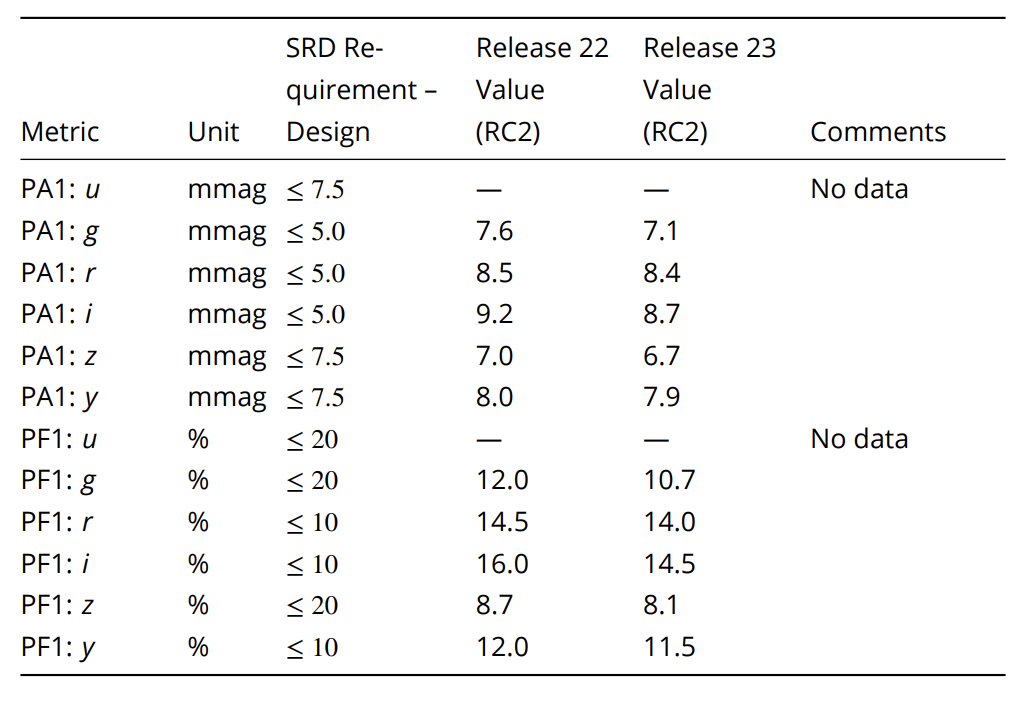
\includegraphics[width=5.15625in]{jira_imgs/3270.png}

}

\paragraph{ LVV-T199 - Verify implementation of Archive Center Co-Location with Existing
Facility }\mbox{}\\

Version \textbf{1}.
Status \textbf{Approved}.
Open  \href{https://jira.lsstcorp.org/secure/Tests.jspa#/testCase/LVV-T199}{\textit{ LVV-T199 } }
test case in Jira.

Verify the Archive Center is located at an existing supported facility.

\textbf{ Preconditions}:\\


Execution status: {\bf Pass }

Final comment:\\


Detailed steps results:

\begin{tabular}{p{2cm}p{14cm}}
\toprule
Step 1 & Step Execution Status: \textbf{ Pass } \\ \hline
\end{tabular}
 Description \\
{\footnotesize
Analyze design

}
\hdashrule[0.5ex]{\textwidth}{1pt}{3mm}
  Expected Result \\
{\footnotesize

}
\hdashrule[0.5ex]{\textwidth}{1pt}{3mm}
  Actual Result \\
{\footnotesize
In \href{http://ls.st/rdo-18}{RDO-18}: PLAN for the OPERATIONS of the
VERA C. RUBIN OBSERVATORY and Execution of its LEGACY SURVEY OF SPACE
AND TIME, the executive summary states (emphasis
added):\\[2\baselineskip]"This operational system will consist of
facilities located at several distinct geographic sites---the Summit
Facility on Cerro Pachón, Chile; the Base Facility in La Serena, Chile;
\emph{the US Data (processing and archiving) Facility at SLAC National
Accelerator Laboratory (SLAC) in California;} the French Data Facility
in Lyon, France; The UK Data Facility in Edinburgh, Scotland; and the
headquarters facility in Tucson, Arizona--as well as the high-speed
networks connecting these sites."\\[2\baselineskip]\ldots{}and in
Section 2.2: An Operations Partnership:\\
``SLAC\ldots{}will continue its managerial role as the lead DOE lab for
operations and will expand its functional role to include camera
maintenance and functional support, participation in assessing and
assuring software, science, and the survey implementation, and operating
the US Data Facility.''\\[2\baselineskip]The following text from Section
9.1.3: Operations Partners highlights the well-established, experienced
nature of SLAC as a DOE lab:\\
``As the lead DOE lab, SLAC will represent and manage contributions from
other DOE labs, including Fermilab, LLNL, and BNL\ldots{} DOE personnel
at SLAC and other laboratories also have extensive experience with data
management and science assurance for large complex instruments and in
other major sky survey projects (e.g., SDSS, Fermi, and DES) that will
translate to Rubin Observatory operations.''

}

\paragraph{ LVV-T190 - Verify implementation of Base Facility Co-Location with Existing
Facility }\mbox{}\\

Version \textbf{1}.
Status \textbf{Approved}.
Open  \href{https://jira.lsstcorp.org/secure/Tests.jspa#/testCase/LVV-T190}{\textit{ LVV-T190 } }
test case in Jira.

Verify that the Base Facility is located at an existing known supported
facility.

\textbf{ Preconditions}:\\


Execution status: {\bf Pass }

Final comment:\\


Detailed steps results:

\begin{tabular}{p{2cm}p{14cm}}
\toprule
Step 1 & Step Execution Status: \textbf{ Pass } \\ \hline
\end{tabular}
 Description \\
{\footnotesize
Analyze design

}
\hdashrule[0.5ex]{\textwidth}{1pt}{3mm}
  Expected Result \\
{\footnotesize

}
\hdashrule[0.5ex]{\textwidth}{1pt}{3mm}
  Actual Result \\
{\footnotesize
In \href{http://ls.st/rdo-18}{RDO-18}: PLAN for the OPERATIONS of the
VERA C. RUBIN OBSERVATORY and Execution of its LEGACY SURVEY OF SPACE
AND TIME, the executive summary states (emphasis
added):\\[2\baselineskip]"This operational system will consist of
facilities located at several distinct geographic sites---the Summit
Facility on Cerro Pachón, Chile; \emph{the Base Facility in La Serena,
Chile;} the US Data (processing and archiving) Facility at SLAC National
Accelerator Laboratory (SLAC) in California; the French Data Facility in
Lyon, France; The UK Data Facility in Edinburgh, Scotland; and the
headquarters facility in Tucson, Arizona--as well as the high-speed
networks connecting these sites."\\[2\baselineskip]The following text
from Section 4.6: Base Facility and Chilean Data Access Center makes it
clear that the Base Facility is co-located with an existing facility
supported by AURA's NOIRLab:\\[2\baselineskip]``The Base Facility is
complete and is a new addition to AURA's NOIRLab La Serena office and
workshop/lab complex called the recinto (in Spanish). The Base Facility
consists of offices for the Observatory Operations department and a
computing facility housed in a 5,000+ square-foot shared computing
center. A dedicated, seismically resistant building with physical access
control, hosts this computing center and supports the computer racks,
power, thermal conditioning, and network routing necessary for
operations\ldots{} A remote control room is part of the facility to
allow remote scientific and technical support of operations on the
summit. Summit monitoring equipment will be remotely operable from the
Base Facility. The La Serena Base computing center will host the Chilean
Data Access Center (DAC) and a backup data archive of the entire LSST
data set\ldots{} Through an agreement with the other AURA centers on the
Recinto, the computing center also will be used to consolidate computing
and network servers from Gemini, CTIO, SOAR, and AURA
operations.''\\[2\baselineskip]

}

\paragraph{ LVV-T77 - Verify implementation of Best Seeing Coadds }\mbox{}\\

Version \textbf{1}.
Status \textbf{Approved}.
Open  \href{https://jira.lsstcorp.org/secure/Tests.jspa#/testCase/LVV-T77}{\textit{ LVV-T77 } }
test case in Jira.

Verify that the DRP pipelines produce a suite of per-band coadds with
input images filtered to optimize the size of the effective PSF on the
coadd.

\textbf{ Preconditions}:\\


Execution status: {\bf Pass }

Final comment:\\The python test script to execute this code is attached to the Test
Report github repository in scripts/test\_LVV-T77.py.


Detailed steps results:

\begin{tabular}{p{2cm}p{14cm}}
\toprule
Step 1 & Step Execution Status: \textbf{ Pass } \\ \hline
\end{tabular}
 Description \\
{\footnotesize
The `path` that you will use depends on where you are running the
science pipelines. Options:\\[2\baselineskip]

\begin{itemize}
\tightlist
\item
  local (newinstall.sh - based
  install):{[}path\_to\_installation{]}/loadLSST.bash
\item
  development cluster (``lsst-dev''):
  /software/lsstsw/stack/loadLSST.bash
\item
  LSP Notebook aspect (from a terminal):
  /opt/lsst/software/stack/loadLSST.bash
\end{itemize}

From the command line, execute the commands below in the example
code:\\[2\baselineskip]

}
\hdashrule[0.5ex]{\textwidth}{1pt}{3mm}
  Example Code \\
{\footnotesize
source `path`\\
setup lsst\_distrib

}
\hdashrule[0.5ex]{\textwidth}{1pt}{3mm}
  Expected Result \\
{\footnotesize
Science pipeline software is available for use. If additional packages
are needed (for example, `obs' packages such as `obs\_subaru`), then
additional `setup` commands will be necessary.\\[2\baselineskip]To check
versions in use, type:\\
eups list -s

}
\hdashrule[0.5ex]{\textwidth}{1pt}{3mm}
  Actual Result \\
{\footnotesize
Test executed on the RSP at the IDF. The test script confirms the
pipelines version by printing the following to the
screen:\\[2\baselineskip]lsst\_distrib g0b29ad24fb+cafeaf151e current
w\_2022\_32 setup

}
\begin{tabular}{p{2cm}p{14cm}}
\toprule
Step 2 & Step Execution Status: \textbf{ Pass } \\ \hline
\end{tabular}
 Description \\
{\footnotesize
Identify the path to the data repository, which we will refer to as
`DATA/path', then execute the following:

}
\hdashrule[0.5ex]{\textwidth}{1pt}{3mm}
  Example Code \\
{\footnotesize
\begin{verbatim}
from lsst.daf.butler import Butler
repo = 'Data/path'
collection = 'collection'
butler = Butler(repo, collections=collection)
\end{verbatim}

}
\hdashrule[0.5ex]{\textwidth}{1pt}{3mm}
  Expected Result \\
{\footnotesize
Butler repo available for reading.

}
\hdashrule[0.5ex]{\textwidth}{1pt}{3mm}
  Actual Result \\
{\footnotesize
We use the DP0.2 data via the following:\\[2\baselineskip]config =
`dp02'\\
collection = `2.2i/runs/DP0.2'\\
butler = Butler(config, collections=collection)

}
\begin{tabular}{p{2cm}p{14cm}}
\toprule
Step 3 & Step Execution Status: \textbf{ Pass } \\ \hline
\end{tabular}
 Description \\
{\footnotesize
Explicitly create a coadd for a specified seeing range in each filter.

}
\hdashrule[0.5ex]{\textwidth}{1pt}{3mm}
  Expected Result \\
{\footnotesize

}
\hdashrule[0.5ex]{\textwidth}{1pt}{3mm}
  Actual Result \\
{\footnotesize
For this test, we extract `goodSeeingCoadd` data products that were
produced during DP0.2 processing.

}
\begin{tabular}{p{2cm}p{14cm}}
\toprule
Step 4 & Step Execution Status: \textbf{ Pass } \\ \hline
\end{tabular}
 Description \\
{\footnotesize
Verify that these coadds exist.

}
\hdashrule[0.5ex]{\textwidth}{1pt}{3mm}
  Expected Result \\
{\footnotesize

}
\hdashrule[0.5ex]{\textwidth}{1pt}{3mm}
  Actual Result \\
{\footnotesize
The test script loops over all ugrizy bands for a single tract/patch,
extracts the `goodSeeingCoadd`, and verifies it is a well-formed image
by printing various statistics to the screen. Finally, the script also
extracts the `deepCoadd\_calexp` image and prints a comparison of the
PSF radius to demonstrate that the best-seeing coadds have a smaller PSF
radius than the deep coadds.\\[2\baselineskip]The output is as
follows:\\[2\baselineskip]Input dataId: \{'tract': 4431, `patch': 17,
`band': `u'\}\\[2\baselineskip]Image shape and statistics:\\
Shape: (4200, 4200)\\
Mean, median, std deviation of pixel values: 0.03438813 0.0024560345
5.8153605\\[2\baselineskip]Variance plane shape and statistics:\\
Shape: (4200, 4200)\\
Mean, median, std deviation of pixel values: 0.020518279 0.019447705
0.10152267\\[2\baselineskip]Mask plane has the following mask bits
set:\\
\{'BAD': 0, `CLIPPED': 9, `CR': 3, `CROSSTALK': 10, `DETECTED': 5,
`DETECTED\_NEGATIVE': 6, `EDGE': 4, `INEXACT\_PSF': 11, `INTRP': 2,
`NOT\_DEBLENDED': 12, `NO\_DATA': 8, `REJECTED': 13, `SAT': 1,
`SENSOR\_EDGE': 14, `SUSPECT': 7, `UNMASKEDNAN': 15\}\\
Mask plane has dimensions: (4200, 4200)\\[2\baselineskip]WCS for
goodSeeingCoadd image with dataId \{'tract': 4431, `patch': 17, `band':
`u'\} :\\
FITS standard SkyWcs:\\
Sky Origin: (55.6521739130, -31.9834710744)\\
Pixel Origin: (13999, 13999)\\
Pixel Scale: 0.2 arcsec/pixel\\[2\baselineskip]Photocalib for
goodSeeingCoadd image with dataId \{'tract': 4431, `patch': 17, `band':
`u'\} :\\
spatially constant with mean: 57.544 error: 0\\[2\baselineskip]Good
seeing coadd PSF radius: 1.7244082609166302\\
Deep coadd PSF radius: 2.074471010117085\\[2\baselineskip]Input dataId:
\{'tract': 4431, `patch': 17, `band': `g'\}\\[2\baselineskip]Image shape
and statistics:\\
Shape: (4200, 4200)\\
Mean, median, std deviation of pixel values: 0.041773453 0.002788621
2.0373423\\[2\baselineskip]Variance plane shape and statistics:\\
Shape: (4200, 4200)\\
Mean, median, std deviation of pixel values: 0.002616897 0.002469438
0.0104264915\\[2\baselineskip]Mask plane has the following mask bits
set:\\
\{'BAD': 0, `CLIPPED': 9, `CR': 3, `CROSSTALK': 10, `DETECTED': 5,
`DETECTED\_NEGATIVE': 6, `EDGE': 4, `INEXACT\_PSF': 11, `INTRP': 2,
`NOT\_DEBLENDED': 12, `NO\_DATA': 8, `REJECTED': 13, `SAT': 1,
`SENSOR\_EDGE': 14, `SUSPECT': 7, `UNMASKEDNAN': 15\}\\
Mask plane has dimensions: (4200, 4200)\\[2\baselineskip]WCS for
goodSeeingCoadd image with dataId \{'tract': 4431, `patch': 17, `band':
`g'\} :\\
FITS standard SkyWcs:\\
Sky Origin: (55.6521739130, -31.9834710744)\\
Pixel Origin: (13999, 13999)\\
Pixel Scale: 0.2 arcsec/pixel\\[2\baselineskip]Photocalib for
goodSeeingCoadd image with dataId \{'tract': 4431, `patch': 17, `band':
`g'\} :\\
spatially constant with mean: 57.544 error: 0\\[2\baselineskip]Good
seeing coadd PSF radius: 1.5164241757236603\\
Deep coadd PSF radius: 1.8854643031757852\\[2\baselineskip]Input dataId:
\{'tract': 4431, `patch': 17, `band': `r'\}\\[2\baselineskip]Image shape
and statistics:\\
Shape: (4200, 4200)\\
Mean, median, std deviation of pixel values: 0.08445272 0.0020215698
2.8918285\\[2\baselineskip]Variance plane shape and statistics:\\
Shape: (4200, 4200)\\
Mean, median, std deviation of pixel values: 0.002568767 0.0024733383
0.011166171\\[2\baselineskip]\hspace*{0.333em}Mask plane has the
following mask bits set:\\
\{'BAD': 0, `CLIPPED': 9, `CR': 3, `CROSSTALK': 10, `DETECTED': 5,
`DETECTED\_NEGATIVE': 6, `EDGE': 4, `INEXACT\_PSF': 11, `INTRP': 2, '\\
NOT\_DEBLENDED': 12, `NO\_DATA': 8, `REJECTED': 13, `SAT': 1,
`SENSOR\_EDGE': 14, `SUSPECT': 7, `UNMASKEDNAN': 15\}\\
Mask plane has dimensions: (4200, 4200)\\[2\baselineskip]WCS for
goodSeeingCoadd image with dataId \{'tract': 4431, `patch': 17, `band':
`r'\} :\\
FITS standard SkyWcs:\\
Sky Origin: (55.6521739130, -31.9834710744)\\
Pixel Origin: (13999, 13999)\\
Pixel Scale: 0.2 arcsec/pixel\\[2\baselineskip]Photocalib for
goodSeeingCoadd image with dataId \{'tract': 4431, `patch': 17, `band':
`r'\} :\\
spatially constant with mean: 57.544 error: 0\\[2\baselineskip]Good
seeing coadd PSF radius: 1.513700867128578\\
Deep coadd PSF radius: 1.8005040445327916\\[2\baselineskip]Input dataId:
\{'tract': 4431, `patch': 17, `band': `i'\}\\[2\baselineskip]Image shape
and statistics:\\
Shape: (4200, 4200)\\
Mean, median, std deviation of pixel values: 0.12454637 0.0037209666
4.126306\\[2\baselineskip]Variance plane shape and statistics:\\
Shape: (4200, 4200)\\
Mean, median, std deviation of pixel values: inf 0.009205212
nan\\[2\baselineskip]Mask plane has the following mask bits set:\\
\{'BAD': 0, `CLIPPED': 9, `CR': 3, `CROSSTALK': 10, `DETECTED': 5,
`DETECTED\_NEGATIVE': 6, `EDGE': 4, `INEXACT\_PSF': 11, `INTRP': 2,
`NOT\_DEBLENDED': 12, `NO\_DATA': 8, `REJECTED': 13, `SAT': 1,
`SENSOR\_EDGE': 14, `SUSPECT': 7, `UNMASKEDNAN': 15\}\\
Mask plane has dimensions: (4200,
4200)\\[2\baselineskip]\hspace*{0.333em}WCS for goodSeeingCoadd image
with dataId ~\{'tract': 4431, `patch': 17, `band': `i'\} :\\
FITS standard SkyWcs:\\
Sky Origin: (55.6521739130, -31.9834710744)\\
Pixel Origin: (13999, 13999)\\
Pixel Scale: 0.2 arcsec/pixel\\[2\baselineskip]Photocalib for
goodSeeingCoadd image with dataId \{'tract': 4431, `patch': 17, `band':
`i'\} :\\
spatially constant with mean: 57.544 error: 0\\[2\baselineskip]Good
seeing coadd PSF radius: 1.5099309000064964\\
Deep coadd PSF radius: 1.728315912605641\\[2\baselineskip]Input dataId:
\{'tract': 4431, `patch': 17, `band': `z'\}\\[2\baselineskip]Image shape
and statistics:\\
Shape: (4200, 4200)\\
Mean, median, std deviation of pixel values: 0.15889181 0.012767363
5.4510126\\[2\baselineskip]Variance plane shape and statistics:\\
Shape: (4200, 4200)\\
Mean, median, std deviation of pixel values: 0.082706526 0.080273375
0.040728822\\[2\baselineskip]Mask plane has the following mask bits
set:\\
\{'BAD': 0, `CLIPPED': 9, `CR': 3, `CROSSTALK': 10, `DETECTED': 5,
`DETECTED\_NEGATIVE': 6, `EDGE': 4, `INEXACT\_PSF': 11, `INTRP': 2,
`NOT\_DEBLENDED': 12, `NO\_DATA': 8, `REJECTED': 13, `SAT': 1,
`SENSOR\_EDGE': 14, `SUSPECT': 7, `UNMASKEDNAN': 15\}\\
Mask plane has dimensions: (4200, 4200)\\[2\baselineskip]WCS for
goodSeeingCoadd image with dataId \{'tract': 4431, `patch': 17, `band':
`z'\} :\\
FITS standard SkyWcs:\\
Sky Origin: (55.6521739130, -31.9834710744)\\
Pixel Origin: (13999, 13999)\\
Pixel Scale: 0.2
arcsec/pixel\\[2\baselineskip]\hspace*{0.333em}Photocalib for
goodSeeingCoadd image with dataId ~\{'tract': 4431, `patch': 17, `band':
`z'\} :\\
spatially constant with mean: 57.544 error: 0\\[2\baselineskip]Good
seeing coadd PSF radius: 1.6839970224085898\\
Deep coadd PSF radius: 1.9398605388502517\\[2\baselineskip]Input dataId:
\{'tract': 4431, `patch': 17, `band': `y'\}\\[2\baselineskip]Image shape
and statistics:\\
Shape: (4200, 4200)\\
Mean, median, std deviation of pixel values: 0.2097747 0.022823093
7.169966\\[2\baselineskip]Variance plane shape and statistics:\\
Shape: (4200, 4200)\\
Mean, median, std deviation of pixel values: 0.26777592 0.26288232
0.16389878\\[2\baselineskip]Mask plane has the following mask bits
set:\\
\{'BAD': 0, `CLIPPED': 9, `CR': 3, `CROSSTALK': 10, `DETECTED': 5,
`DETECTED\_NEGATIVE': 6, `EDGE': 4, `INEXACT\_PSF': 11, `INTRP': 2,
`NOT\_DEBLENDED': 12, `NO\_DATA': 8, `REJECTED': 13, `SAT': 1,
`SENSOR\_EDGE': 14, `SUSPECT': 7, `UNMASKEDNAN': 15\}\\
Mask plane has dimensions: (4200, 4200)\\[2\baselineskip]WCS for
goodSeeingCoadd image with dataId \{'tract': 4431, `patch': 17, `band':
`y'\} :\\
FITS standard SkyWcs:\\
Sky Origin: (55.6521739130, -31.9834710744)\\
Pixel Origin: (13999, 13999)\\
Pixel Scale: 0.2 arcsec/pixel\\[2\baselineskip]Photocalib for
goodSeeingCoadd image with dataId \{'tract': 4431, `patch': 17, `band':
`y'\} :\\
spatially constant with mean: 57.544 error: 0\\[2\baselineskip]Good
seeing coadd PSF radius: 2.2861573969027273\\
Deep coadd PSF radius: 2.508081993634421

}

\paragraph{ LVV-T84 - Verify implementation of Bias Residual Image }\mbox{}\\

Version \textbf{1}.
Status \textbf{Approved}.
Open  \href{https://jira.lsstcorp.org/secure/Tests.jspa#/testCase/LVV-T84}{\textit{ LVV-T84 } }
test case in Jira.

Verify that DMS can construct a bias residual image that corrects for
temporally-stable bias structures.\\
Verify that DMS can do this on demand.

\textbf{ Preconditions}:\\


Execution status: {\bf Pass }

Final comment:\\Results are in the notebook ``test\_LVV-T84.ipynb'' attached to the Test
Report repository.


Detailed steps results:

\begin{tabular}{p{2cm}p{14cm}}
\toprule
Step 1 & Step Execution Status: \textbf{ Pass } \\ \hline
\end{tabular}
 Description \\
{\footnotesize
Identify the location of an appropriate precursor dataset.

}
\hdashrule[0.5ex]{\textwidth}{1pt}{3mm}
  Expected Result \\
{\footnotesize

}
\hdashrule[0.5ex]{\textwidth}{1pt}{3mm}
  Actual Result \\
{\footnotesize
Working on the Rubin Science Platform (RSP) hosted at the USDF (SLAC),
using Science Pipelines version w\_2022\_32.\\[2\baselineskip]The
HSC/RC2 dataset we will use is in a shared repository at:\\
repo = `/sdf/group/rubin/repo/main'\\
collection = `HSC/runs/RC2/w\_2022\_28/DM-35609'

}
\begin{tabular}{p{2cm}p{14cm}}
\toprule
Step 2 & Step Execution Status: \textbf{ Pass } \\ \hline
\end{tabular}
 Description \\
{\footnotesize
Identify the path to the data repository, which we will refer to as
`DATA/path', then execute the following:

}
\hdashrule[0.5ex]{\textwidth}{1pt}{3mm}
  Example Code \\
{\footnotesize
\begin{verbatim}
from lsst.daf.butler import Butler
repo = 'Data/path'
collection = 'collection'
butler = Butler(repo, collections=collection)
\end{verbatim}

}
\hdashrule[0.5ex]{\textwidth}{1pt}{3mm}
  Expected Result \\
{\footnotesize
Butler repo available for reading.

}
\hdashrule[0.5ex]{\textwidth}{1pt}{3mm}
  Actual Result \\
{\footnotesize
butler = Butler(repo, collections=collection), where the repo and
collection were specified in Step 1.

}
\begin{tabular}{p{2cm}p{14cm}}
\toprule
Step 3 & Step Execution Status: \textbf{ Pass } \\ \hline
\end{tabular}
 Description \\
{\footnotesize
Import the standard libraries required for the rest of this test:

}
\hdashrule[0.5ex]{\textwidth}{1pt}{3mm}
  Example Code \\
{\footnotesize
import os\\
import lsst.afw.display as afwDisplay\\
from lsst.daf.persistence import Butler\\
from lsst.ip.isr import IsrTask

}
\hdashrule[0.5ex]{\textwidth}{1pt}{3mm}
  Expected Result \\
{\footnotesize

}
\hdashrule[0.5ex]{\textwidth}{1pt}{3mm}
  Actual Result \\
{\footnotesize
LIbraries imported.

}
\begin{tabular}{p{2cm}p{14cm}}
\toprule
Step 4 & Step Execution Status: \textbf{ Pass } \\ \hline
\end{tabular}
 Description \\
{\footnotesize
Ingest the dataset from step 1 using the Butler (e.g., following example
code below).

}
\hdashrule[0.5ex]{\textwidth}{1pt}{3mm}
  Example Code \\
{\footnotesize
butler = Butler(\$REPOSITORY\_PATH)\\
raw = butler.get(тАЬrawтАЭ, visit=\$VISIT\_ID, detector=2)\\
bias = butler.get(тАЬbiasтАЭ, visit=\$VISIT\_ID, detector=2)

}
\hdashrule[0.5ex]{\textwidth}{1pt}{3mm}
  Expected Result \\
{\footnotesize

}
\hdashrule[0.5ex]{\textwidth}{1pt}{3mm}
  Actual Result \\
{\footnotesize
In our case, we specified a full dataId for a single i-band visit, then
retrieved the corresponding raw and bias images:\\[2\baselineskip]dataId
= \{'instrument': `HSC', `detector': 42, `visit': 30482,
`exposure':30482, `band':'i'\}\\
raw = butler.get('raw', dataId=dataId)\\
bias = butler.get('bias', dataId=dataId)

}
\begin{tabular}{p{2cm}p{14cm}}
\toprule
Step 5 & Step Execution Status: \textbf{ Pass } \\ \hline
\end{tabular}
 Description \\
{\footnotesize
Display the bias image and inspect that its pixels contain unique
values.

}
\hdashrule[0.5ex]{\textwidth}{1pt}{3mm}
  Expected Result \\
{\footnotesize
A relatively flat image showing the bias level with roughly Poisson
noise.

}
\hdashrule[0.5ex]{\textwidth}{1pt}{3mm}
  Actual Result \\
{\footnotesize
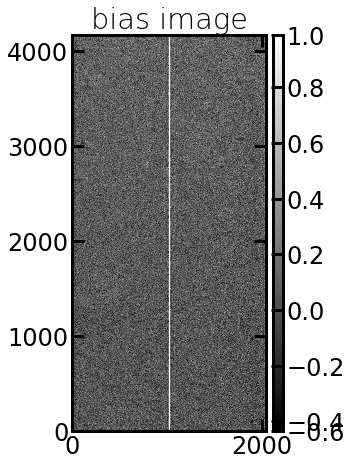
\includegraphics[width=3.12500in]{jira_imgs/3055.png}

}
\begin{tabular}{p{2cm}p{14cm}}
\toprule
Step 6 & Step Execution Status: \textbf{ Pass } \\ \hline
\end{tabular}
 Description \\
{\footnotesize
Configure and run an Instrument Signature Removal (ISR) task on the raw
data. Most corrections are disabled for simplicity, but the bias frame
is applied.\\[2\baselineskip]

}
\hdashrule[0.5ex]{\textwidth}{1pt}{3mm}
  Example Code \\
{\footnotesize
isr\_config = IsrTask.ConfigClass()\\
isr\_config.doDark=False\\
isr\_config.doFlat=False\\
isr\_config.doFringe=False\\
isr\_config.doDefect=False\\
isr\_config.doLinearize=False\\
isr = IsrTask(config=isr\_config)\\
result = isr.run(raw, bias=bias, detectorNum=raw.detector.getId(),
camera=obs\_lsst.LsstCamImSim.getCamera())

}
\hdashrule[0.5ex]{\textwidth}{1pt}{3mm}
  Expected Result \\
{\footnotesize
A trimmed, bias-corrected image in `result`.

}
\hdashrule[0.5ex]{\textwidth}{1pt}{3mm}
  Actual Result \\
{\footnotesize
The ``result'' image was returned. To confirm the bias subtraction had
the desired effect, we printed some statistics to the
screen:\\[2\baselineskip]

\begin{verbatim}
  image       median     stddev    (of image pixel values)
bias:        0.07311707 0.23739594
raw:         8130.0 2496.6898982587295
after bias:  6802.6895 895.51544
\end{verbatim}

The noise is reduced significantly, suggesting the bias had its intended
effect.

}
\begin{tabular}{p{2cm}p{14cm}}
\toprule
Step 7 & Step Execution Status: \textbf{ Pass } \\ \hline
\end{tabular}
 Description \\
{\footnotesize
Display the `result` image and confirm that the bias correction has been
performed.

}
\hdashrule[0.5ex]{\textwidth}{1pt}{3mm}
  Expected Result \\
{\footnotesize
A displayed image with bias removed (i.e., typical background counts
reduced relative to the raw frame).

}
\hdashrule[0.5ex]{\textwidth}{1pt}{3mm}
  Actual Result \\
{\footnotesize
This image displays the raw frame on the left, and the same image after
bias subtraction on the right.\\
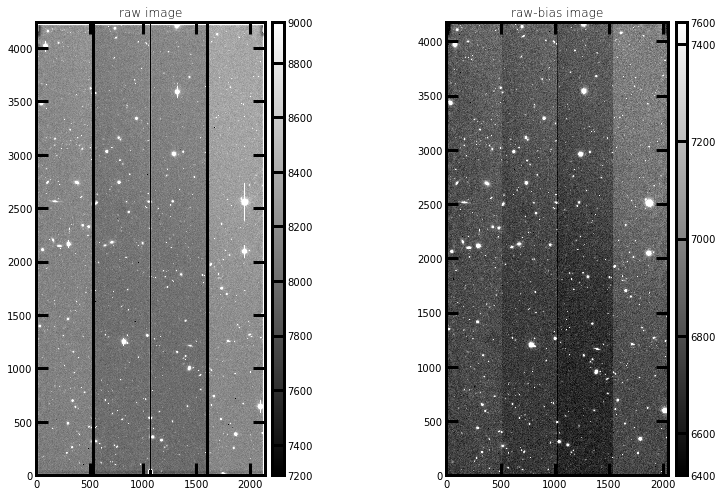
\includegraphics[width=3.75000in]{jira_imgs/3056.png}\\
We have thus demonstrated that the bias correction can be applied on
demand.

}

\paragraph{ LVV-T151 - Verify Implementation of Catalog Export Formats From the Notebook Aspect }\mbox{}\\

Version \textbf{1}.
Status \textbf{Approved}.
Open  \href{https://jira.lsstcorp.org/secure/Tests.jspa#/testCase/LVV-T151}{\textit{ LVV-T151 } }
test case in Jira.

Verify that catalog data is exportable from the notebook aspect in a
variety of community-standard formats.

\textbf{ Preconditions}:\\


Execution status: {\bf Pass }

Final comment:\\Results of the test execution can be found in the notebook
``test\_LVV-T151.ipynb'' attached to the github repository.


Detailed steps results:

\begin{tabular}{p{2cm}p{14cm}}
\toprule
Step 1 & Step Execution Status: \textbf{ Pass } \\ \hline
\end{tabular}
 Description \\
{\footnotesize
Authenticate to the notebook aspect of the Rubin Science Platform
(NB-RSP). This is currently at either \url{https://data.lsst.cloud/nb}
(for the interim data facility, or IDF) or
\url{https://usdf-rsp.slac.stanford.edu/nb} (for the US data facility,
or USDF).

}
\hdashrule[0.5ex]{\textwidth}{1pt}{3mm}
  Expected Result \\
{\footnotesize
Redirection to the spawner page of the NB-RSP allowing selection of the
containerized science pipelines version and machine flavor.

}
\hdashrule[0.5ex]{\textwidth}{1pt}{3mm}
  Actual Result \\
{\footnotesize
Arrived at the spawner page.

}
\begin{tabular}{p{2cm}p{14cm}}
\toprule
Step 2 & Step Execution Status: \textbf{ Pass } \\ \hline
\end{tabular}
 Description \\
{\footnotesize
Spawn a container by:\\
1) choosing an appropriate science pipelines version: e.g. the latest
weekly.\\
2) choosing an appropriate machine flavor: e.g. medium\\
3) click ``Spawn''

}
\hdashrule[0.5ex]{\textwidth}{1pt}{3mm}
  Expected Result \\
{\footnotesize
Redirection to the JupyterLab environment served from the chosen
container containing the correct science pipelines version.

}
\hdashrule[0.5ex]{\textwidth}{1pt}{3mm}
  Actual Result \\
{\footnotesize
Spawned a ``medium'' container with Science Pipelines weekly version
w\_2022\_32.

}
\begin{tabular}{p{2cm}p{14cm}}
\toprule
Step 3 & Step Execution Status: \textbf{ Pass } \\ \hline
\end{tabular}
 Description \\
{\footnotesize
Open a new launcher by navigating in the top menu bar ``File''
-\textgreater{} ``New Launcher''

}
\hdashrule[0.5ex]{\textwidth}{1pt}{3mm}
  Expected Result \\
{\footnotesize
A launcher window with several sections, potentially with several kernel
versions for each.

}
\hdashrule[0.5ex]{\textwidth}{1pt}{3mm}
  Actual Result \\
{\footnotesize
Launcher appeared, with notebook, terminal, and other options.

}
\begin{tabular}{p{2cm}p{14cm}}
\toprule
Step 4 & Step Execution Status: \textbf{ Pass } \\ \hline
\end{tabular}
 Description \\
{\footnotesize
Select the option under ``Notebook'' labeled ``LSST'' by clicking on the
icon.

}
\hdashrule[0.5ex]{\textwidth}{1pt}{3mm}
  Expected Result \\
{\footnotesize
An empty notebook with a single empty cell. ~The kernel show up as
``LSST'' in the top right of the notebook.

}
\hdashrule[0.5ex]{\textwidth}{1pt}{3mm}
  Actual Result \\
{\footnotesize
Notebook appeared with w\_2022\_32 loaded, and an LSST kernel.

}
\begin{tabular}{p{2cm}p{14cm}}
\toprule
Step 5 & Step Execution Status: \textbf{ Pass } \\ \hline
\end{tabular}
 Description \\
{\footnotesize
Execute a query in a notebook to select a small number of stars. In the
example code below, we query the Data Preview 0.2 (DP0.2) catalog, then
extract the results to an Astropy table.

}
\hdashrule[0.5ex]{\textwidth}{1pt}{3mm}
  Example Code \\
{\footnotesize
\begin{verbatim}
CELL 1:

from IPython.display import Markdown as md
from lsst.rsp import get_tap_service, retrieve_query
    
service = get_tap_service()
md(f'The service endpoint for TAP in this environment is:\n\n &#10145;&nbsp;&nbsp;   {service.baseurl}')

CELL 2:

results = service.search("SELECT coord_ra, coord_dec, g_cModelFlux, r_cModelFlux \
                          FROM dp02_dc2_catalogs.Object \
                          WHERE CONTAINS(POINT('ICRS', coord_ra, coord_dec), \
                          CIRCLE('ICRS', 60.0, -30.0, 0.05)) = 1")
\end{verbatim}

}
\hdashrule[0.5ex]{\textwidth}{1pt}{3mm}
  Expected Result \\
{\footnotesize
Screen output from CELL 1:\\[2\baselineskip]The service endpoint for TAP
in this environment is:\\
➡ \url{https://data.lsst.cloud/api/tap}\\[2\baselineskip]Example screen
output from CELL 2 (may not contain the same 10
entries):\\[2\baselineskip]\emph{Table length=5533}

coord\_ra

coord\_dec

g\_cModelFlux

r\_cModelFlux

deg

deg

nJy

nJy

float64

float64

float64

float64

59.9987401

-29.9728812

62.7060123

49.3496319

59.9995813

-29.9743232

166.0433743

394.8261645

59.9989853

-29.9750457

78.9557388

85.2691232

59.9993731

-29.9732406

111.0082072

165.6229656

60.0477786

-29.9736805

68.4818592

49.4783714

60.0400024

-29.9731507

52.0567337

114.2562171

60.0054666

-29.9728639

146.053072

134.1795803

60.00489

-29.9732239

1436.7150639

3606.8163133

60.0469583

-29.9735655

64.8838762

56.5677789

\ldots{}

\ldots{}

\ldots{}

\ldots{}

60.0053313

-30.0240394

125.6977786

379.8120713

59.9574061

-30.0163726

181.050889

200.8032979

60.0294415

-30.0241709

133.662163

230.8673464

59.9563419

-30.0239843

1551.2308712

4611.0406542

59.9879157

-30.0181116

76.3796313

46.5682713

60.0204061

-30.0228981

174.7738892

304.9991558

60.001638

-30.0183336

43.9593753

46.9695823

59.9861714

-30.0173405

164.6261404

288.8650875

59.9537443

-30.0160515

2228.7204658

5091.2041475

59.9683498

-30.0239539

835.415374

1101.0548649

\begin{longtable}[]{@{}ll@{}}
\toprule
&\tabularnewline
\bottomrule
\end{longtable}

}
\hdashrule[0.5ex]{\textwidth}{1pt}{3mm}
  Actual Result \\
{\footnotesize
The following was printed to the screen after CELL
1:\\[2\baselineskip]The service endpoint for TAP in this environment
is:\\
➡ ~~\url{https://data.lsst.cloud/api/tap}\\[2\baselineskip]After
executing CELL 2, converted the results to an Astropy table using `tab =
results.to\_table()`

}
\begin{tabular}{p{2cm}p{14cm}}
\toprule
Step 6 & Step Execution Status: \textbf{ Pass } \\ \hline
\end{tabular}
 Description \\
{\footnotesize
Using the example code below, save the files to your storage space on
the RSP Notebook Aspect.\\[2\baselineskip]Confirm that non-empty output
files appear on disk.

}
\hdashrule[0.5ex]{\textwidth}{1pt}{3mm}
  Example Code \\
{\footnotesize
tab.write('test.csv', format='ascii.csv')\\
tab.write('test.vot', format='votable')\\
tab.write('test.fits', format='fits')

}
\hdashrule[0.5ex]{\textwidth}{1pt}{3mm}
  Expected Result \\
{\footnotesize
For the example given here, there should be the following files with the
file size as listed:

\begin{itemize}
\tightlist
\item
  test.csv 5.7M
\item
  test.vot 16M
\item
  test.fits 4.5M
\end{itemize}

}
\hdashrule[0.5ex]{\textwidth}{1pt}{3mm}
  Actual Result \\
{\footnotesize
Upon executing, the three output files appear in the file browser on the
left side of the screen. We checked the file output sizes in a Terminal
window using `ls -ltrh test.*`\\[2\baselineskip]Output:\\
-rw-r--r-- 1 jeffcarlin 309K Aug 24 17:17 test.csv\\
-rw-r--r-- 1 jeffcarlin 829K Aug 24 17:17 test.vot\\
-rw-r--r-- 1 jeffcarlin 225K Aug 24 17:17 test.fits

}
\begin{tabular}{p{2cm}p{14cm}}
\toprule
Step 7 & Step Execution Status: \textbf{ Pass } \\ \hline
\end{tabular}
 Description \\
{\footnotesize
Check that these files contain the same number of rows:

}
\hdashrule[0.5ex]{\textwidth}{1pt}{3mm}
  Example Code \\
{\footnotesize
from astropy.table import Table\\
dat\_csv = Table.read('test.csv', format='ascii.csv')\\
dat\_vot = Table.read('test.vot', format='votable')\\
dat\_fits = Table.read('test.fits',
format='fits')\\[2\baselineskip]import numpy as np\\
print(np.size(dat\_csv), np.size(dat\_vot), np.size(dat\_fits))

}
\hdashrule[0.5ex]{\textwidth}{1pt}{3mm}
  Expected Result \\
{\footnotesize
Print statement produces output ``5533 5533 5533''.

}
\hdashrule[0.5ex]{\textwidth}{1pt}{3mm}
  Actual Result \\
{\footnotesize
As expected, the screen output was:

\begin{verbatim}
5533 5533 5533
\end{verbatim}

}
\begin{tabular}{p{2cm}p{14cm}}
\toprule
Step 8 & Step Execution Status: \textbf{ Pass } \\ \hline
\end{tabular}
 Description \\
{\footnotesize
Under the `File' menu at the top of your Jupyter notebook session,
select one of the following:\\[2\baselineskip]

\begin{itemize}
\tightlist
\item
  Save All, Exit, and Log Out
\item
  Exit and Log Out Without Saving
\end{itemize}

}
\hdashrule[0.5ex]{\textwidth}{1pt}{3mm}
  Expected Result \\
{\footnotesize
You will be returned to the RSP landing page: either
\url{https://data.lsst.cloud/nb} (for the interim data facility, or IDF)
or \url{https://usdf-rsp.slac.stanford.edu/nb} (for the US data
facility, or USDF). It is now safe to close the browser window.

}
\hdashrule[0.5ex]{\textwidth}{1pt}{3mm}
  Actual Result \\
{\footnotesize
Successfully logged out and returned to the landing page.

}

\paragraph{ LVV-T1232 - Verify Implementation of Catalog Export Formats From the Portal Aspect }\mbox{}\\

Version \textbf{1}.
Status \textbf{Approved}.
Open  \href{https://jira.lsstcorp.org/secure/Tests.jspa#/testCase/LVV-T1232}{\textit{ LVV-T1232 } }
test case in Jira.

Verify that catalog data is exportable from the portal aspect in a
variety of community-standard formats.

\textbf{ Preconditions}:\\


Execution status: {\bf Pass }

Final comment:\\


Detailed steps results:

\begin{tabular}{p{2cm}p{14cm}}
\toprule
Step 1 & Step Execution Status: \textbf{ Pass } \\ \hline
\end{tabular}
 Description \\
{\footnotesize
Navigate to the Portal Aspect endpoint. ~The stable version at the
interim data facility (IDF) should be used for this test and is
currently located at: \url{https://data.lsst.cloud/portal/app}.

}
\hdashrule[0.5ex]{\textwidth}{1pt}{3mm}
  Expected Result \\
{\footnotesize
A credential-entry screen should be displayed.

}
\hdashrule[0.5ex]{\textwidth}{1pt}{3mm}
  Actual Result \\
{\footnotesize
Clicked on the ``login'' button at upper right, and authenticated via
github credentials.

}
\begin{tabular}{p{2cm}p{14cm}}
\toprule
Step 2 & Step Execution Status: \textbf{ Pass } \\ \hline
\end{tabular}
 Description \\
{\footnotesize
Enter a valid set of credentials for an LSST user with RSP access on the
instance under test.

}
\hdashrule[0.5ex]{\textwidth}{1pt}{3mm}
  Expected Result \\
{\footnotesize
The Portal Aspect UI should be displayed following authentication.

}
\hdashrule[0.5ex]{\textwidth}{1pt}{3mm}
  Actual Result \\
{\footnotesize
The Portal Aspect is displayed.

}
\begin{tabular}{p{2cm}p{14cm}}
\toprule
Step 3 & Step Execution Status: \textbf{ Pass } \\ \hline
\end{tabular}
 Description \\
{\footnotesize
Select query type ``ADQL''.

}
\hdashrule[0.5ex]{\textwidth}{1pt}{3mm}
  Expected Result \\
{\footnotesize

}
\hdashrule[0.5ex]{\textwidth}{1pt}{3mm}
  Actual Result \\
{\footnotesize
Selected ``Edit ADQL'' in box number 2. Box 1 default -- ``LSST RSP
https://data.lsst.cloud/api/tap'' is retained.

}
\begin{tabular}{p{2cm}p{14cm}}
\toprule
Step 4 & Step Execution Status: \textbf{ Pass } \\ \hline
\end{tabular}
 Description \\
{\footnotesize
Execute the example query given in the example code below by entering
the text in the ADQL Query box, then clicking ``Search'' at the lower
left corner of the page.

}
\hdashrule[0.5ex]{\textwidth}{1pt}{3mm}
  Example Code \\
{\footnotesize
\begin{verbatim}
SELECT coord_ra, coord_dec, g_cModelFlux, r_cModelFlux FROM dp02_dc2_catalogs.Object WHERE CONTAINS(POINT('ICRS', coord_ra, coord_dec), CIRCLE('ICRS', 60.0, -30.0, 0.05)) = 1
\end{verbatim}

}
\hdashrule[0.5ex]{\textwidth}{1pt}{3mm}
  Expected Result \\
{\footnotesize
A new page will load with the search results as a table, with some plots
as well.

}
\hdashrule[0.5ex]{\textwidth}{1pt}{3mm}
  Actual Result \\
{\footnotesize
The following page loaded, showing 5533 results from the query:\\
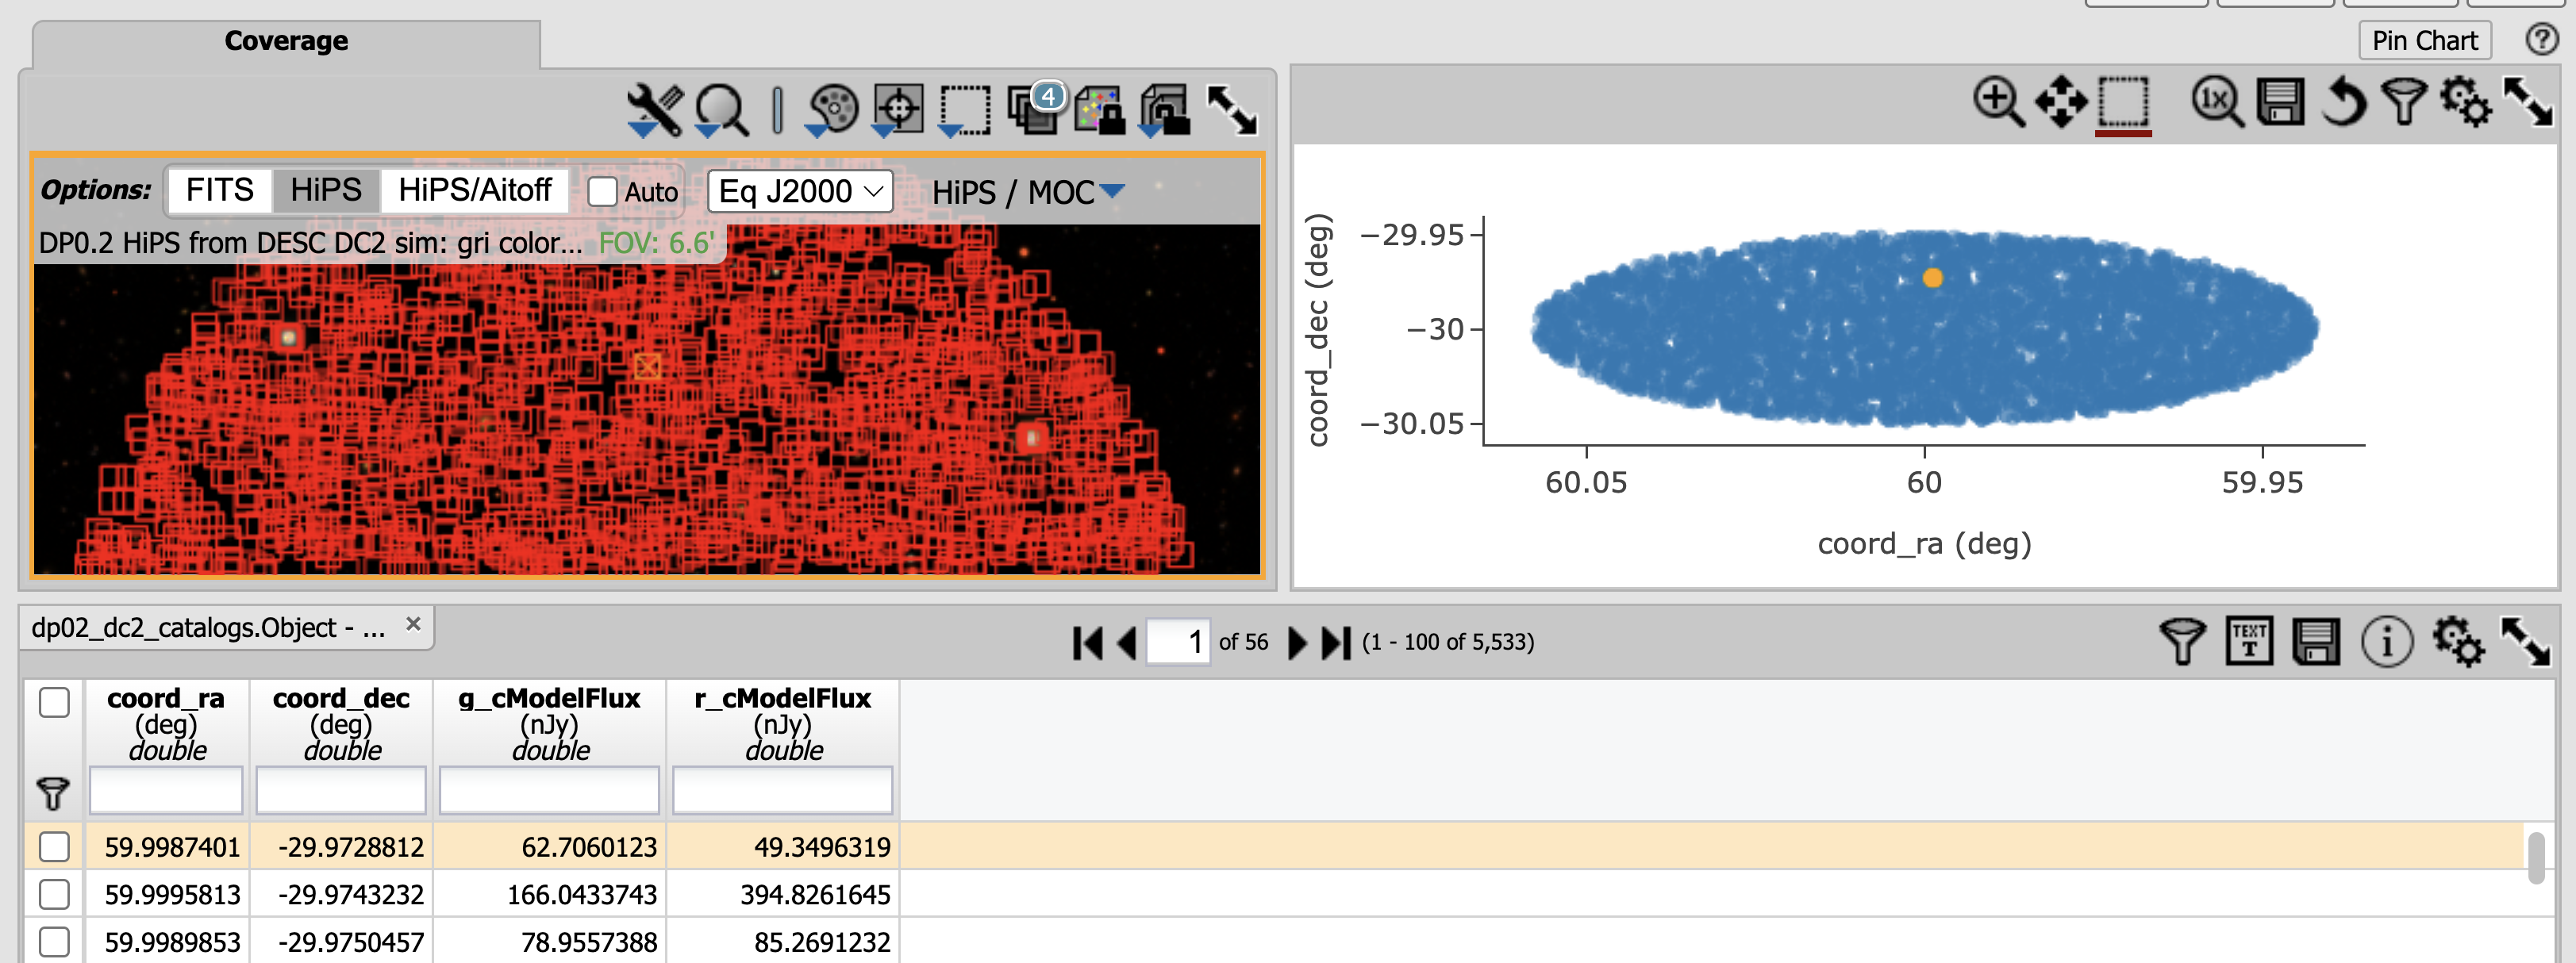
\includegraphics[width=5.08333in]{jira_imgs/3046.png}

}
\begin{tabular}{p{2cm}p{14cm}}
\toprule
Step 5 & Step Execution Status: \textbf{ Pass } \\ \hline
\end{tabular}
 Description \\
{\footnotesize
Click the icon that looks like a floppy disk (it says ``Save the content
as an IPAC, CSV, or TSV table'' when you mouse over it).

}
\hdashrule[0.5ex]{\textwidth}{1pt}{3mm}
  Expected Result \\
{\footnotesize

}
\hdashrule[0.5ex]{\textwidth}{1pt}{3mm}
  Actual Result \\
{\footnotesize
File save menu appeared.

}
\begin{tabular}{p{2cm}p{14cm}}
\toprule
Step 6 & Step Execution Status: \textbf{ Pass } \\ \hline
\end{tabular}
 Description \\
{\footnotesize
\begin{itemize}
\tightlist
\item
  Select ``CSV'', then specify a destination to save the file on your
  local computer.
\item
  Select ``VOTable'', then specify a destination to save the file on
  your local computer.
\item
  Select ``FITS'', then specify a destination to save the file on your
  local computer.
\end{itemize}

}
\hdashrule[0.5ex]{\textwidth}{1pt}{3mm}
  Expected Result \\
{\footnotesize

}
\hdashrule[0.5ex]{\textwidth}{1pt}{3mm}
  Actual Result \\
{\footnotesize
\emph{NOTE: the option to export as FITS-binary-table (i.e., .fits) is
not currently supported by the Portal. We used ``VOTable - FITS'' for
this execution, but if it is expected that FITS will be supported in the
future, this test should be executed again to verify FITS export.\\
}\\
After saving in all three formats to a local computer, executed the
following:\\[2\baselineskip]`ls -ltrh test*`\\[2\baselineskip]Output:\\
-rw-r--r--@ 1 jcarlin staff 253K Aug 24 10:44
test\_LVV-T1232\_dp02\_catalog.csv\\
-rw-r--r--@ 1 jcarlin staff 610K Aug 24 10:45
test\_LVV-T1232\_dp02\_catalog.vot\\
-rw-r--r--@ 1 jcarlin staff 245K Aug 24 10:45
test\_LVV-T1232\_dp02\_catalog.fits.vot\\[2\baselineskip]

}
\begin{tabular}{p{2cm}p{14cm}}
\toprule
Step 7 & Step Execution Status: \textbf{ Pass } \\ \hline
\end{tabular}
 Description \\
{\footnotesize
Open each of the files (either in TOPCAT, or using Astropy io tools).
Confirm that the data tables are well-formed, and that each table
contains the same columns and the same number of rows.

}
\hdashrule[0.5ex]{\textwidth}{1pt}{3mm}
  Expected Result \\
{\footnotesize

}
\hdashrule[0.5ex]{\textwidth}{1pt}{3mm}
  Actual Result \\
{\footnotesize
Opening each file in TOPCAT, we confirmed that all three of them have
5533 rows, and 4 columns.

}
\begin{tabular}{p{2cm}p{14cm}}
\toprule
Step 8 & Step Execution Status: \textbf{ Pass } \\ \hline
\end{tabular}
 Description \\
{\footnotesize
Click the ``logout'' button at the upper right corner of the Portal
screen.

}
\hdashrule[0.5ex]{\textwidth}{1pt}{3mm}
  Expected Result \\
{\footnotesize
Returned to the RSP home page at
\href{https://data.lsst.cloud/}{https://data.lsst.cloud/.} When
navigating to the portal endpoint, expect to execute the steps in
LVV-T849.

}
\hdashrule[0.5ex]{\textwidth}{1pt}{3mm}
  Actual Result \\
{\footnotesize
Returned to the RSP home page.

}

\paragraph{ LVV-T72 - Verify implementation of Coadd Image Method Constraints }\mbox{}\\

Version \textbf{1}.
Status \textbf{Approved}.
Open  \href{https://jira.lsstcorp.org/secure/Tests.jspa#/testCase/LVV-T72}{\textit{ LVV-T72 } }
test case in Jira.

Verify the implementation of how Coadd images are created.

\textbf{ Preconditions}:\\


Execution status: {\bf Pass }

Final comment:\\The executed notebook was saved in the repository associated with this
campaign's test report as ``notebooks/test\_LVV-T72.ipynb''.


Detailed steps results:

\begin{tabular}{p{2cm}p{14cm}}
\toprule
Step 1 & Step Execution Status: \textbf{ Pass } \\ \hline
\end{tabular}
 Description \\
{\footnotesize
Identify a dataset that has been processed to create coadd images.

}
\hdashrule[0.5ex]{\textwidth}{1pt}{3mm}
  Expected Result \\
{\footnotesize

}
\hdashrule[0.5ex]{\textwidth}{1pt}{3mm}
  Actual Result \\
{\footnotesize
We will use the Data Preview 0.2 dataset as processed at the Interim
Data Facility (IDF).

}
\begin{tabular}{p{2cm}p{14cm}}
\toprule
Step 2 & Step Execution Status: \textbf{ Pass } \\ \hline
\end{tabular}
 Description \\
{\footnotesize
Identify the path to the data repository, which we will refer to as
`DATA/path', then execute the following:

}
\hdashrule[0.5ex]{\textwidth}{1pt}{3mm}
  Example Code \\
{\footnotesize
\begin{verbatim}
from lsst.daf.butler import Butler
repo = 'Data/path'
collection = 'collection'
butler = Butler(repo, collections=collection)
\end{verbatim}

}
\hdashrule[0.5ex]{\textwidth}{1pt}{3mm}
  Expected Result \\
{\footnotesize
Butler repo available for reading.

}
\hdashrule[0.5ex]{\textwidth}{1pt}{3mm}
  Actual Result \\
{\footnotesize
Working in a notebook entitled ``test\_LVV-T72.ipynb'' on the Interim
Data Facility at data.lsst.cloud:\\[2\baselineskip]from lsst.daf.butler
import Butler\\[2\baselineskip]config = `dp02'\\
collection = `2.2i/runs/DP0.2'\\
butler = Butler(config, collections=collection)

}
\begin{tabular}{p{2cm}p{14cm}}
\toprule
Step 3 & Step Execution Status: \textbf{ Pass } \\ \hline
\end{tabular}
 Description \\
{\footnotesize
Retrieve the coadds in the dataset and verify that they are non-empty.

}
\hdashrule[0.5ex]{\textwidth}{1pt}{3mm}
  Expected Result \\
{\footnotesize

}
\hdashrule[0.5ex]{\textwidth}{1pt}{3mm}
  Actual Result \\
{\footnotesize
First, we query the Butler to find all coadds overlapping the requested
tract:\\[2\baselineskip]tract = 3828\\[2\baselineskip]data\_refs\_coadd
= butler.registry.queryDatasets(\\
datasetType=``deepCoadd'',\\
where=f``tract=\{tract\} and
skymap='DC2''')\\[2\baselineskip]data\_ids\_coadd =
{[}{]}\\[2\baselineskip]for data\_ref in data\_refs\_coadd:\\
data\_ids\_coadd.append(data\_ref.dataId.full)\\[2\baselineskip]We
examined a few images at random, and confirmed they are non-empty and
contained all necessary associated data by printing the following output
to the screen (see the notebook for more detail):\\

\begin{verbatim}
dataId:  {band: 'i', skymap: 'DC2', tract: 3828, patch: 1}

 Image shape and statistics:
Shape:  (4100, 4200)
Mean, median, std deviation of pixel values:  0.08778822 -0.00036619927 4.830672

 Variance plane shape and statistics:
Shape:  (4100, 4200)
Median of pixel values:  0.0033457286

 Mask plane has the following mask bits set:
{'BAD': 0, 'CLIPPED': 9, 'CR': 3, 'CROSSTALK': 10, 'DETECTED': 5, 'DETECTED_NEGATIVE': 6, 'EDGE': 4, 'INEXACT_PSF': 11, 'INTRP': 2, 'NOT_DEBLENDED': 12, 'NO_DATA': 8, 'REJECTED': 13, 'SAT': 1, 'SENSOR_EDGE': 14, 'SUSPECT': 7, 'UNMASKEDNAN': 15}
Mask plane has dimensions:  (4200, 4100)

Has PSF?  True

 WCS:
FITS standard SkyWcs:
Sky Origin: (56.6497461929, -36.4462809917)
Pixel Origin: (13999, 13999)
Pixel Scale: 0.2 arcsec/pixel

 Photocalib:
spatially constant with mean: 57.544 error: 0
\end{verbatim}

}
\begin{tabular}{p{2cm}p{14cm}}
\toprule
Step 4 & Step Execution Status: \textbf{ Pass } \\ \hline
\end{tabular}
 Description \\
{\footnotesize
Verify that coadds were created following specification

}
\hdashrule[0.5ex]{\textwidth}{1pt}{3mm}
  Expected Result \\
{\footnotesize

}
\hdashrule[0.5ex]{\textwidth}{1pt}{3mm}
  Actual Result \\
{\footnotesize
To verify that the coadds have been created using all of the overlapping
visit images, we extract the catalog of overlapping images and plot
their bounding boxes along with that of the coadd. Details can be seen
in the attached notebook, which produced this
image:\\[2\baselineskip]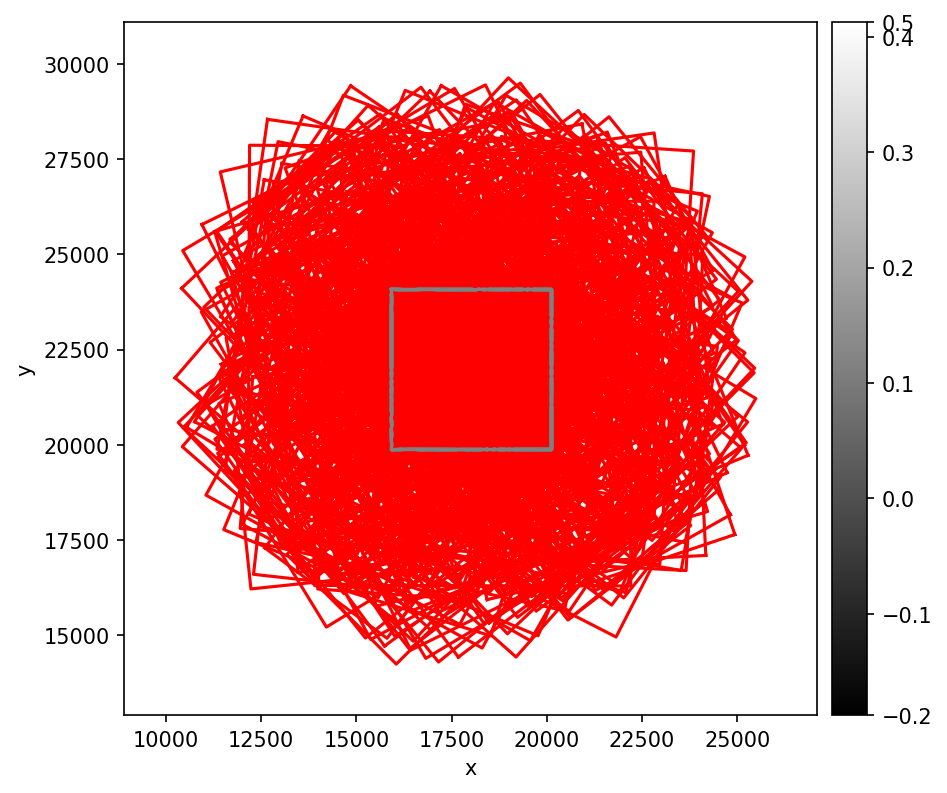
\includegraphics[width=3.86458in]{jira_imgs/3315.png}We
have thus verified that the randomly-selected coadd was created
following specification.

}

\paragraph{ LVV-T90 - Verify implementation of Dark Current Correction Frame }\mbox{}\\

Version \textbf{1}.
Status \textbf{Approved}.
Open  \href{https://jira.lsstcorp.org/secure/Tests.jspa#/testCase/LVV-T90}{\textit{ LVV-T90 } }
test case in Jira.

Verify that the DMS can produce a dark correction frame calibration
product.

\textbf{ Preconditions}:\\


Execution status: {\bf Pass }

Final comment:\\Results are in the notebook ``test\_LVV-T90.ipynb'' attached to the Test
Report repository.


Detailed steps results:

\begin{tabular}{p{2cm}p{14cm}}
\toprule
Step 1 & Step Execution Status: \textbf{ Pass } \\ \hline
\end{tabular}
 Description \\
{\footnotesize
Identify the path to a dataset containing dark frames (i.e., exposures
taken with the shutter closed).

}
\hdashrule[0.5ex]{\textwidth}{1pt}{3mm}
  Expected Result \\
{\footnotesize

}
\hdashrule[0.5ex]{\textwidth}{1pt}{3mm}
  Actual Result \\
{\footnotesize
Working on the Rubin Science Platform (RSP) hosted at the USDF (SLAC),
using Science Pipelines version w\_2022\_32.\\[2\baselineskip]The
HSC/RC2 dataset we will use is in a shared repository at:\\
repo = `/sdf/group/rubin/repo/main'\\
collection = `HSC/runs/RC2/w\_2022\_28/DM-35609'

}
\begin{tabular}{p{2cm}p{14cm}}
\toprule
Step 2 & Step Execution Status: \textbf{ Pass } \\ \hline
\end{tabular}
 Description \\
{\footnotesize
Execute the relevant steps from `cp\_pipe` (the calibration pipeline) to
produce dark correction frames.

}
\hdashrule[0.5ex]{\textwidth}{1pt}{3mm}
  Expected Result \\
{\footnotesize

}
\hdashrule[0.5ex]{\textwidth}{1pt}{3mm}
  Actual Result \\
{\footnotesize
The ISR correction steps have been executed during the bi-weekly RC2
reprocessing campaign.

}
\begin{tabular}{p{2cm}p{14cm}}
\toprule
Step 3 & Step Execution Status: \textbf{ Pass } \\ \hline
\end{tabular}
 Description \\
{\footnotesize
Inspect the resulting dark correction frame to confirm that it appears
as expected.

}
\hdashrule[0.5ex]{\textwidth}{1pt}{3mm}
  Expected Result \\
{\footnotesize
A well-formed dark correction frame is present and accessible via the
Data Butler.

}
\hdashrule[0.5ex]{\textwidth}{1pt}{3mm}
  Actual Result \\
{\footnotesize
The following image was retrieved from the Butler. It looks like a
well-formed image, and shows some minor features and the bottom-middle
region.\\
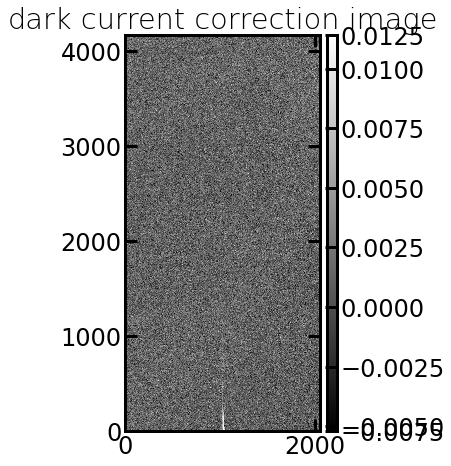
\includegraphics[width=3.12500in]{jira_imgs/3057.png}

}

\paragraph{ LVV-T137 - Verify implementation of Data Product Ingest }\mbox{}\\

Version \textbf{1}.
Status \textbf{Approved}.
Open  \href{https://jira.lsstcorp.org/secure/Tests.jspa#/testCase/LVV-T137}{\textit{ LVV-T137 } }
test case in Jira.

Verify that data products can be ingested.

\textbf{ Preconditions}:\\


Execution status: {\bf Pass }

Final comment:\\


Detailed steps results:

\begin{tabular}{p{2cm}p{14cm}}
\toprule
Step 1 & Step Execution Status: \textbf{ Pass } \\ \hline
\end{tabular}
 Description \\
{\footnotesize
Identify a suitable set of raw data to be run through ``mini-DRP''
processing.

}
\hdashrule[0.5ex]{\textwidth}{1pt}{3mm}
  Expected Result \\
{\footnotesize

}
\hdashrule[0.5ex]{\textwidth}{1pt}{3mm}
  Actual Result \\
{\footnotesize
This test will be executed using the
\href{https://github.com/lsst-dm/rc2_subset}{rc2\_subset} data, which is
a curated dataset selected to allow for full end-to-end processing of
all DRP steps. The test will be executed on the USDF (SLAC) development
machines, using Science Pipelines version w\_2022\_30.

}
\begin{tabular}{p{2cm}p{14cm}}
\toprule
Step 2 & Step Execution Status: \textbf{ Pass } \\ \hline
\end{tabular}
 Description \\
{\footnotesize
Process data with the Data Release Production payload, starting from raw
science images and generating science data products, placing them in the
Data Backbone.

}
\hdashrule[0.5ex]{\textwidth}{1pt}{3mm}
  Expected Result \\
{\footnotesize

}
\hdashrule[0.5ex]{\textwidth}{1pt}{3mm}
  Actual Result \\
{\footnotesize
The shell script used to execute the steps of DRP processing is as
follows:\\[2\baselineskip]\# Set up Stack\\
\# source /opt/lsst/software/stack/loadLSST.bash\\
source
/cvmfs/sw.lsst.eu/linux-x86\_64/lsst\_distrib/w\_2022\_30/loadLSST.bash\\
setup lsst\_distrib\\
eups list -s \textbar{} grep lsst\_distrib\\[2\baselineskip]\#cd
\$HOME/DATA\\
cd /sdf/group/rubin/sandbox/\$USER\\
\#git clone https://github.com/lsst-dm/rc2\_subset\\
cd repos\\
setup -j -r rc2\_subset\\
echo \$RC2\_SUBSET\_DIR\\[2\baselineskip]export
NUMPROC=8\\[2\baselineskip]pipetask --long-log run -j \$NUMPROC -b
\$\{RC2\_SUBSET\_DIR\}/SMALL\_HSC/butler.yaml -p
\$\{RC2\_SUBSET\_DIR\}'/pipelines/DRP.yaml\#nightlyStep1' -i
HSC/RC2/defaults --register-dataset-types -o
u/\$USER/step1\\[2\baselineskip]echo ``Running step2a on all visits''\\
pipetask --long-log run -j \$NUMPROC -b
\$\{RC2\_SUBSET\_DIR\}/SMALL\_HSC/butler.yaml -p
\$\{RC2\_SUBSET\_DIR\}'/pipelines/DRP.yaml\#nightlyStep2a' -i
u/\$USER/step1 --register-dataset-types -o
u/\$USER/step2\\[2\baselineskip]echo ``Running step2b on tract 9813''\\
pipetask --long-log run -j \$NUMPROC -b
\$\{RC2\_SUBSET\_DIR\}/SMALL\_HSC/butler.yaml -p
\$\{RC2\_SUBSET\_DIR\}'/pipelines/DRP.yaml\#nightlyStep2b' -d ``tract =
9813 and skymap = `hsc\_rings\_v1'\,'' --register-dataset-types -o
u/\$USER/step2\\[2\baselineskip]echo ``Running step2c without
multiprocessing''\\
pipetask --long-log run -b \$\{RC2\_SUBSET\_DIR\}/SMALL\_HSC/butler.yaml
-p \$\{RC2\_SUBSET\_DIR\}'/pipelines/DRP.yaml\#nightlyStep2c'
--register-dataset-types -o u/\$USER/step2\\[2\baselineskip]echo
``Running step2d on all visits''\\
pipetask --long-log run -j \$NUMPROC -b
\$\{RC2\_SUBSET\_DIR\}/SMALL\_HSC/butler.yaml -p
\$\{RC2\_SUBSET\_DIR\}'/pipelines/DRP.yaml\#nightlyStep2d'
--register-dataset-types -o u/\$USER/step2\\[2\baselineskip]echo
``Running step3 on all visits''\\
pipetask --long-log run -j \$NUMPROC -b
\$\{RC2\_SUBSET\_DIR\}/SMALL\_HSC/butler.yaml -p
\$\{RC2\_SUBSET\_DIR\}'/pipelines/DRP.yaml\#nightlyStep3' -d ``tract =
9813 and skymap = `hsc\_rings\_v1' AND patch in (38, 39, 40, 41)'' -i
u/\$USER/step2 --register-dataset-types -o
u/\$USER/step3\\[2\baselineskip]echo ``Running step4 on all visits''\\
pipetask --long-log run -j \$NUMPROC -b
\$\{RC2\_SUBSET\_DIR\}/SMALL\_HSC/butler.yaml -p
\$\{RC2\_SUBSET\_DIR\}'/pipelines/DRP.yaml\#nightlyStep4' -d ``tract =
9813 and skymap = `hsc\_rings\_v1' AND patch in (38, 39, 40, 41)'' -i
u/\$USER/step3 --register-dataset-types -o
u/\$USER/step4\\[2\baselineskip]

}
\begin{tabular}{p{2cm}p{14cm}}
\toprule
Step 3 & Step Execution Status: \textbf{ Pass } \\ \hline
\end{tabular}
 Description \\
{\footnotesize
Identify the path to the data repository, which we will refer to as
`DATA/path', then execute the following:

}
\hdashrule[0.5ex]{\textwidth}{1pt}{3mm}
  Example Code \\
{\footnotesize
\begin{verbatim}
from lsst.daf.butler import Butler
repo = 'Data/path'
collection = 'collection'
butler = Butler(repo, collections=collection)
\end{verbatim}

}
\hdashrule[0.5ex]{\textwidth}{1pt}{3mm}
  Expected Result \\
{\footnotesize
Butler repo available for reading.

}
\hdashrule[0.5ex]{\textwidth}{1pt}{3mm}
  Actual Result \\
{\footnotesize
See the attached script, ``test\_LVV-T137.py'', which contains the
following lines to initialize the Butler:\\[2\baselineskip]from
lsst.daf.butler import Butler\\[2\baselineskip]repo =
`/sdf/group/rubin/u/jcarlin/repos/rc2\_subset/SMALL\_HSC'\\
collection~=~'u/jcarlin/step4'\\
butler~= Butler(repo, collections=collection)\\[2\baselineskip]

}
\begin{tabular}{p{2cm}p{14cm}}
\toprule
Step 4 & Step Execution Status: \textbf{ Pass } \\ \hline
\end{tabular}
 Description \\
{\footnotesize
Confirm that the data products from the DRP processing have been
ingested into the Data Backbone.

}
\hdashrule[0.5ex]{\textwidth}{1pt}{3mm}
  Expected Result \\
{\footnotesize
Processed images, catalogs, calibration information, and other related
data products are present and accessible via the Butler.

}
\hdashrule[0.5ex]{\textwidth}{1pt}{3mm}
  Actual Result \\
{\footnotesize
The attached script, ``test\_LVV-T137.py'' was executed from the command
line via ``python test\_LVV-T137.py \textgreater{} test\_LVV-T137.out''.
The screen output demonstrates that calibrated exposures have been
created from ingested raws and calibration frames, and source detection
and measurement has been performed (among other processing). The output
of the script is (note: we have truncated the schema results for the
``src'' catalog for readability):\\[2\baselineskip]lsst\_distrib
g0b29ad24fb+434521fcbd current w\_2022\_35 setup\\
WCS for calexp image with dataId \{'instrument': `HSC', `detector': 42,
`visit': 19680\} :\\
FITS standard SkyWcs:\\
Sky Origin: (149.9670716242, +2.1456871368)\\
Pixel Origin: (989.716, 2019.07)\\
Pixel Scale: 0.168409 arcsec/pixel\\
Photocalib for calexp image with dataId \{'instrument': `HSC',
`detector': 42, `visit': 19680\} :\\
spatially constant with mean: 0.199449 error: 0.000171253\\
Image shape and statistics:\\
Shape: (4176, 2048)\\
Mean, median, std deviation of pixel values: 21.659693 3.1226554
277.56586\\
Variance plane shape and statistics:\\
Shape: (4176, 2048)\\
Mean, median, std deviation of pixel values: 918.03143 841.7631
476.36658\\
Mask plane has the following mask bits set:\\
\{'BAD': 0, `CR': 3, `CROSSTALK': 9, `DETECTED': 5,
`DETECTED\_NEGATIVE': 6, `EDGE': 4, `INTRP': 2, `NOT\_DEBLENDED': 10,
`NO\_DATA': 8, `SAT': 1, `SUSPECT': 7, `UNMASKEDNAN': 11\}\\
Mask plane has dimensions: (2048, 4176)\\
Source catalog has 5135 entries.\\
The first five entries in the source catalog:\\
id coord\_ra \ldots{} calib\_photometry\_reserved\\
rad \ldots{}\\
---------------- ------------------ \ldots{} -------------------------\\
8452585832841217 2.615778319777679 \ldots{} False\\
8452585832841218 2.6157771306147075 \ldots{} False\\
8452585832841219 2.6157783826078296 \ldots{} False\\
8452585832841220 2.6157761384385596 \ldots{} False\\
8452585832841221 2.6157747119184185 \ldots{} False\\
The schema of the source catalog:\\
Schema(\\
(Field{[}'L'{]}(name=``id'', doc=``unique ID''),
Key\textless{}L\textgreater{}(offset=0, nElements=1)),\\
(Field{[}'Angle'{]}(name=``coord\_ra'', doc=``position in ra/dec''),
Key\textless{}Angle\textgreater{}(offset=8, nElements=1)),\\
(Field{[}'Angle'{]}(name=``coord\_dec'', doc=``position in ra/dec''),
Key\textless{}Angle\textgreater{}(offset=16, nElements=1)),\\
(Field{[}'L'{]}(name=``parent'', doc=``unique ID of parent source''),
Key\textless{}L\textgreater{}(offset=24, nElements=1)),\\
(Field{[}'Flag'{]}(name=``calib\_detected'', doc=``Source was detected
as an icSource''), Key{[}'Flag'{]}(offset=32, bit=0)),\\
(Field{[}'Flag'{]}(name=``calib\_psf\_candidate'', doc=``Flag set if the
source was a candidate for PSF determination, as determined by the star
selector.''), Key{[}'Flag'{]}(offset=32, bit=1)),\\
(Field{[}'Flag'{]}(name=``calib\_psf\_used'', doc=``Flag set if the
source was actually used for PSF determination, as determined by the''),
Key{[}'Flag'{]}(offset=32, bit=2)),\\
(Field{[}'Flag'{]}(name=``calib\_psf\_reserved'', doc=``set if source
was reserved from PSF determination''), Key{[}'Flag'{]}(offset=32,
bit=3)),\\
(Field{[}'I'{]}(name=``deblend\_nChild'', doc=``Number of children this
object has (defaults to 0)''), Key\textless{}I\textgreater{}(offset=40,
nElements=1)),\\
(Field{[}'Flag'{]}(name=``deblend\_deblendedAsPsf'', doc=``Deblender
thought this source looked like a PSF''), Key{[}'Flag'{]}(offset=32,
bit=4)),\\
(Field{[}'D'{]}(name=``deblend\_psfCenter\_x'', doc=``If
deblended-as-psf, the PSF centroid'', units=``pixel''),
Key\textless{}D\textgreater{}(offset=48, nElements=1)),\\
(Field{[}'D'{]}(name=``deblend\_psfCenter\_y'', doc=``If
deblended-as-psf, the PSF centroid'', units=``pixel''),
Key\textless{}D\textgreater{}(offset=56, nElements=1)),\\
(Field{[}'D'{]}(name=``deblend\_psf\_instFlux'', doc=``If
deblended-as-psf, the instrumental PSF flux'', units=``count''),
Key\textless{}D\textgreater{}(offset=64,
nElements=1)),\\[2\baselineskip]\ldots{}\\[2\baselineskip](Field{[}'D'{]}(name=``ext\_photometryKron\_KronFlux\_apCorrErr'',
doc=``standard deviation of aperture correction applied to
ext\_photometryKron\_KronFlux''),
Key\textless{}D\textgreater{}(offset=992, nElements=1)),\\
(Field{[}'Flag'{]}(name=``ext\_photometryKron\_KronFlux\_flag\_apCorr'',
doc=``set if unable to aperture correct
ext\_photometryKron\_KronFlux''), Key{[}'Flag'{]}(offset=976, bit=1)),\\
(Field{[}'D'{]}(name=``base\_ClassificationExtendedness\_value'',
doc=``Set to 1 for extended sources, 0 for point sources.''),
Key\textless{}D\textgreater{}(offset=1000, nElements=1)),\\
(Field{[}'Flag'{]}(name=``base\_ClassificationExtendedness\_flag'',
doc=``Set to 1 for any fatal failure.''), Key{[}'Flag'{]}(offset=976,
bit=2)),\\
(Field{[}'I'{]}(name=``base\_FootprintArea\_value'', doc=``Number of
pixels in the source''s detection footprint.'', units=``pixel''),
Key\textless{}I\textgreater{}(offset=1008, nElements=1)),\\
(Field{[}'Flag'{]}(name=``calib\_astrometry\_used'', doc=``set if source
was used in astrometric calibration''), Key{[}'Flag'{]}(offset=976,
bit=3)),\\
(Field{[}'Flag'{]}(name=``calib\_photometry\_used'', doc=``set if source
was used in photometric calibration''), Key{[}'Flag'{]}(offset=976,
bit=4)),\\
(Field{[}'Flag'{]}(name=``calib\_photometry\_reserved'', doc=``set if
source was reserved from photometric calibration''),
Key{[}'Flag'{]}(offset=976, bit=5)),\\
`base\_CircularApertureFlux\_flag\_badCentroid'-\textgreater{}'base\_SdssCentroid\_flag'\\
`base\_GaussianFlux\_flag\_badCentroid'-\textgreater{}'base\_SdssCentroid\_flag'\\
`base\_GaussianFlux\_flag\_badShape'-\textgreater{}'ext\_shapeHSM\_HsmSourceMoments\_flag'\\
`base\_LocalBackground\_flag\_badCentroid'-\textgreater{}'base\_SdssCentroid\_flag'\\
`base\_NaiveCentroid\_flag\_badInitialCentroid'-\textgreater{}'base\_SdssCentroid\_flag'\\
`base\_PsfFlux\_flag\_badCentroid'-\textgreater{}'base\_SdssCentroid\_flag'\\
`base\_SdssShape\_flag\_badCentroid'-\textgreater{}'base\_SdssCentroid\_flag'\\
`base\_Variance\_flag\_badCentroid'-\textgreater{}'base\_SdssCentroid\_flag'\\
`ext\_photometryKron\_KronFlux\_flag\_badInitialCentroid'-\textgreater{}'base\_SdssCentroid\_flag'\\
`ext\_shapeHSM\_HsmPsfMomentsDebiased\_flag\_badCentroid'-\textgreater{}'base\_SdssCentroid\_flag'\\
`ext\_shapeHSM\_HsmPsfMoments\_flag\_badCentroid'-\textgreater{}'base\_SdssCentroid\_flag'\\
`ext\_shapeHSM\_HsmShapeRegauss\_flag\_badCentroid'-\textgreater{}'base\_SdssCentroid\_flag'\\
`ext\_shapeHSM\_HsmSourceMomentsRound\_flag\_badCentroid'-\textgreater{}'base\_SdssCentroid\_flag'\\
`ext\_shapeHSM\_HsmSourceMoments\_flag\_badCentroid'-\textgreater{}'base\_SdssCentroid\_flag'\\
`slot\_ApFlux'-\textgreater{}'base\_CircularApertureFlux\_12\_0'\\
`slot\_CalibFlux'-\textgreater{}'base\_CircularApertureFlux\_12\_0'\\
`slot\_Centroid'-\textgreater{}'base\_SdssCentroid'\\
`slot\_GaussianFlux'-\textgreater{}'base\_GaussianFlux'\\
`slot\_ModelFlux'-\textgreater{}'base\_GaussianFlux'\\
`slot\_PsfFlux'-\textgreater{}'base\_PsfFlux'\\
`slot\_PsfShape'-\textgreater{}'ext\_shapeHSM\_HsmPsfMoments'\\
`slot\_Shape'-\textgreater{}'ext\_shapeHSM\_HsmSourceMoments'\\
)\\[2\baselineskip]Median of PSF magnitudes calculated using the
associated PhotoCalib object:\\
24.88843561504042\\[2\baselineskip]

}

\paragraph{ LVV-T55 - Verify implementation of DIAForcedSource Catalog }\mbox{}\\

Version \textbf{1}.
Status \textbf{Approved}.
Open  \href{https://jira.lsstcorp.org/secure/Tests.jspa#/testCase/LVV-T55}{\textit{ LVV-T55 } }
test case in Jira.

Verify that the DMS produces a DIAForcedSource Catalog and that the
catalog contains measured fluxes for DIAObjects.

\textbf{ Preconditions}:\\


Execution status: {\bf Pass }

Final comment:\\The python test script to execute this code is attached to the Test
Report github repository in scripts/test\_LVV-T55.py.


Detailed steps results:

\begin{tabular}{p{2cm}p{14cm}}
\toprule
Step 1 & Step Execution Status: \textbf{ Pass } \\ \hline
\end{tabular}
 Description \\
{\footnotesize
Perform the steps of Alert Production (including, but not necessarily
limited to, single frame processing, ISR, source detection/measurement,
PSF estimation, photometric and astrometric calibration, difference
imaging, DIASource detection/measurement, source association). During
Operations, it is presumed that these are automated for a given
dataset.~

}
\hdashrule[0.5ex]{\textwidth}{1pt}{3mm}
  Expected Result \\
{\footnotesize
An output dataset including difference images and DIASource and
DIAObject measurements.

}
\hdashrule[0.5ex]{\textwidth}{1pt}{3mm}
  Actual Result \\
{\footnotesize
For this test, we use the monthly reprocessing of the HSC RC2 dataset.
All steps of end-to-end data processing are executed in the RC2 runs,
including difference imaging.

}
\begin{tabular}{p{2cm}p{14cm}}
\toprule
Step 2 & Step Execution Status: \textbf{ Pass } \\ \hline
\end{tabular}
 Description \\
{\footnotesize
Verify that the expected data products have been produced, and that
catalogs contain reasonable values for measured quantities of interest.

}
\hdashrule[0.5ex]{\textwidth}{1pt}{3mm}
  Expected Result \\
{\footnotesize

}
\hdashrule[0.5ex]{\textwidth}{1pt}{3mm}
  Actual Result \\
{\footnotesize
Load and inspect the `forcedSourceOnDiaObjectTable` to confirm that it
was produced and all columns have been populated with
measurements:\\[2\baselineskip]In {[}\textbf{11}{]}:~forced\_src =
butler.get('forcedSourceOnDiaObjectTable\_tract', tract=9615,
skymap='hsc\_rings\_v1')\\[2\baselineskip]In {[}12{]}:~forced\_src\\
Out{[}12{]}:~\\
\hspace*{0.333em} ~ ~ ~ ~ ~ ~ ~ ~ ~ ~ ~ ~ ~ ~ ~ ~
~diaObjectId~~parentObjectId~
~~coord\_ra~~coord\_dec~~ccdVisitId~~\ldots{}
pixelFlags\_saturatedCenter~~pixelFlags\_crCenter~~pixelFlags\_suspectCenter~~tract~~patch\\
forcedSourceOnDiaObjectId~ ~ ~ ~ ~ ~ ~ ~ ~ ~ ~ ~ ~ ~ ~ ~ ~ ~ ~ ~ ~ ~ ~ ~
~ ~ ~ ~ ~ ~ ~ ~ ~ ~ ~ ~ ~~\ldots{} ~ ~ ~ ~ ~ ~ ~ ~ ~ ~ ~ ~ ~ ~ ~ ~ ~ ~ ~
~ ~ ~ ~ ~ ~ ~ ~ ~ ~ ~ ~ ~ ~ ~ ~ ~ ~ ~ ~ ~ ~ ~ ~ ~\\
173516678758401~ ~ ~ ~ ~ ~~3425330564243128393 ~ ~ ~ ~ ~ ~
~~0~~215.886840 ~~0.254806 ~ ~ ~~80800~~\ldots{}~ ~ ~ ~ ~ ~ ~ ~ ~ ~
~~False~ ~ ~ ~ ~ ~ ~ ~~False ~ ~ ~ ~ ~ ~ ~ ~ ~ ~~False ~~9615 ~ ~~15\\
173516678758402~ ~ ~ ~ ~ ~~3425330564243128394 ~ ~ ~ ~ ~ ~
~~0~~215.889248 ~~0.247669 ~ ~ ~~80800~~\ldots{}~ ~ ~ ~ ~ ~ ~ ~ ~ ~
~~False~ ~ ~ ~ ~ ~ ~ ~~False ~ ~ ~ ~ ~ ~ ~ ~ ~ ~~False ~~9615 ~ ~~15\\
173516678758403~ ~ ~ ~ ~ ~~3425330564243128395 ~ ~ ~ ~ ~ ~
~~0~~215.889644 ~~0.241762 ~ ~ ~~80800~~\ldots{}~ ~ ~ ~ ~ ~ ~ ~ ~ ~
~~False~ ~ ~ ~ ~ ~ ~ ~~False ~ ~ ~ ~ ~ ~ ~ ~ ~ ~~False ~~9615 ~ ~~15\\
173516678758404~ ~ ~ ~ ~ ~~3425330564243128399 ~ ~ ~ ~ ~ ~
~~0~~215.897606 ~~0.244158 ~ ~ ~~80800~~\ldots{}~ ~ ~ ~ ~ ~ ~ ~ ~ ~
~~False~ ~ ~ ~ ~ ~ ~ ~~False ~ ~ ~ ~ ~ ~ ~ ~ ~ ~~False ~~9615 ~
~~15\\[2\baselineskip]{[}39147253 rows x 34
columns{]}\\[2\baselineskip]The table looks well-formed.

}
\begin{tabular}{p{2cm}p{14cm}}
\toprule
Step 3 & Step Execution Status: \textbf{ Pass } \\ \hline
\end{tabular}
 Description \\
{\footnotesize
Identify the path to the data repository, which we will refer to as
`DATA/path', then execute the following:

}
\hdashrule[0.5ex]{\textwidth}{1pt}{3mm}
  Example Code \\
{\footnotesize
\begin{verbatim}
from lsst.daf.butler import Butler
repo = 'Data/path'
collection = 'collection'
butler = Butler(repo, collections=collection)
\end{verbatim}

}
\hdashrule[0.5ex]{\textwidth}{1pt}{3mm}
  Expected Result \\
{\footnotesize
Butler repo available for reading.

}
\hdashrule[0.5ex]{\textwidth}{1pt}{3mm}
  Actual Result \\
{\footnotesize
Working on the USDF (SLAC), a butler was instantiated by the
following:\\[2\baselineskip]repo = `/sdf/group/rubin/repo/main'\\
collection = `HSC/runs/RC2/w\_2022\_24/DM-35231'\\
butler = Butler(repo, collections=collection)\\[2\baselineskip](i.e.,
pointing to processing of HSC RC2 data from weekly w\_2022\_24).

}
\begin{tabular}{p{2cm}p{14cm}}
\toprule
Step 4 & Step Execution Status: \textbf{ Pass } \\ \hline
\end{tabular}
 Description \\
{\footnotesize
Confirm that the DIAForcedSource catalog contains measurements for each
source.

}
\hdashrule[0.5ex]{\textwidth}{1pt}{3mm}
  Expected Result \\
{\footnotesize

}
\hdashrule[0.5ex]{\textwidth}{1pt}{3mm}
  Actual Result \\
{\footnotesize
This test was executed via a script (``test\_LVV-T55.py'') that does the
following:

\begin{itemize}
\tightlist
\item
  Execute a butler query to identify all visit/detector images
  overlapping a given tract/patch
\item
  extract all `forced\_src` catalogs from the query results, and confirm
  that each has (a) forced photometry measurements for each DIAObject
  within its boundaries, and (b) the measurements consist of real
  numbers (i.e., not NaN or Inf).
\end{itemize}

These steps are then repeated for forced photometry on DiaObjects
measured on `calexps`, then difference images. The code prints the
following output:\\[2\baselineskip]\$ python test\_LVV-T55.py\\
lsst\_distrib~ ~ ~ ~ ~~g0b29ad24fb+a10408d0bf~ ~~w\_2022\_39 setup\\
100~~of~~358\\
200~~of~~358\\
300~~of~~358\\[2\baselineskip]Results for~~334 visit/detectors that
overlap the input tract.\\[2\baselineskip]DIA psfflux check:~~True\\
DIA psfflux\_err check:~~True\\
DIA: All objects have forced sources?~~True\\
100~~of~~358\\
200~~of~~358\\
300~~of~~358\\[2\baselineskip]Results for~~334 visit/detectors that
overlap the input tract.\\[2\baselineskip]DIA diffim psfflux
check:~~True\\
DIA diffim psfflux\_err check:~~True\\
DIA diffim: All objects have forced sources? True\\[2\baselineskip]This
confirms that the forced source measurements have been performed for all
DIAObjects, including on `calexps` and `diffims`.\\[2\baselineskip]

}

\paragraph{ LVV-T66 - Verify implementation of Forced-Source Catalog }\mbox{}\\

Version \textbf{1}.
Status \textbf{Approved}.
Open  \href{https://jira.lsstcorp.org/secure/Tests.jspa#/testCase/LVV-T66}{\textit{ LVV-T66 } }
test case in Jira.

Verify that all ForcedSources produced by the DRP pipelines contain
fluxes measured on difference and direct single-epoch images, associated
uncertainties, an Object ID, and a Visit ID.

\textbf{ Preconditions}:\\


Execution status: {\bf Pass }

Final comment:\\The python test script to execute this code is attached to the Test
Report github repository in scripts/test\_LVV-T66.py.


Detailed steps results:

\begin{tabular}{p{2cm}p{14cm}}
\toprule
Step 1 & Step Execution Status: \textbf{ Pass } \\ \hline
\end{tabular}
 Description \\
{\footnotesize
Identify the path to the data repository, which we will refer to as
`DATA/path', then execute the following:

}
\hdashrule[0.5ex]{\textwidth}{1pt}{3mm}
  Example Code \\
{\footnotesize
\begin{verbatim}
from lsst.daf.butler import Butler
repo = 'Data/path'
collection = 'collection'
butler = Butler(repo, collections=collection)
\end{verbatim}

}
\hdashrule[0.5ex]{\textwidth}{1pt}{3mm}
  Expected Result \\
{\footnotesize
Butler repo available for reading.

}
\hdashrule[0.5ex]{\textwidth}{1pt}{3mm}
  Actual Result \\
{\footnotesize
Working on the USDF (SLAC), a butler was instantiated by the
following:\\[2\baselineskip]repo = `/sdf/group/rubin/repo/main'\\
collection = `HSC/runs/RC2/w\_2022\_24/DM-35231'\\
butler = Butler(repo, collections=collection)\\[2\baselineskip](i.e.,
pointing to processing of HSC RC2 data from weekly w\_2022\_24).

}
\begin{tabular}{p{2cm}p{14cm}}
\toprule
Step 2 & Step Execution Status: \textbf{ Pass } \\ \hline
\end{tabular}
 Description \\
{\footnotesize
Retrieve the forced-source catalog from the Butler and verify it to be
non-empty.

}
\hdashrule[0.5ex]{\textwidth}{1pt}{3mm}
  Expected Result \\
{\footnotesize

}
\hdashrule[0.5ex]{\textwidth}{1pt}{3mm}
  Actual Result \\
{\footnotesize
Result of printing the `forced\_src` catalog's first few rows to the
screen:\\[2\baselineskip]\hspace*{0.333em} ~ ~ ~id ~ ~ ~ ~ ~ ~~coord\_ra
~ ~ ~ ~ ~~coord\_dec ~ ~ ~~parent \ldots{} base\_PsfFlux\_flag\_apCorr
ext\_photometryKron\_KronFlux\_apCorr
ext\_photometryKron\_KronFlux\_apCorrErr
ext\_photometryKron\_KronFlux\_flag\_apCorr\\
\hspace*{0.333em} ~ ~ ~ ~ ~ ~ ~ ~ ~ ~ ~~rad ~ ~ ~ ~ ~ ~ ~ ~~rad ~ ~ ~ ~
~ ~ ~ ~~\ldots{} ~ ~ ~ ~ ~ ~ ~ ~ ~ ~ ~ ~ ~ ~ ~ ~ ~ ~ ~ ~ ~ ~ ~ ~ ~ ~ ~ ~
~ ~ ~ ~ ~ ~ ~ ~ ~ ~ ~ ~ ~ ~ ~ ~ ~ ~ ~ ~ ~ ~ ~ ~ ~ ~ ~ ~ ~ ~ ~ ~ ~ ~ ~ ~
~ ~ ~ ~ ~\\
---------------- ------------------ -------------------- ------ \ldots{}
------------------------ ----------------------------------
-------------------------------------
---------------------------------------\\
5029488307994625 ~~2.63104145229885 0.038054902578442455~ ~ ~~0
\ldots{}~ ~ ~ ~ ~ ~ ~ ~ ~ ~~False ~ ~ ~ ~ ~ ~ ~ ~~1.0270320546384992 ~ ~
~ ~ ~ ~ ~ ~ ~ ~ ~ ~ ~ ~ ~ ~ ~~0.0 ~ ~ ~ ~ ~ ~ ~ ~ ~ ~ ~ ~ ~ ~ ~ ~
~~False\\
5029488307994626~~2.630928461400815 0.037891765102001845~ ~ ~~0
\ldots{}~ ~ ~ ~ ~ ~ ~ ~ ~ ~~False~ ~ ~ ~ ~ ~ ~ ~ ~~1.026189759742002 ~ ~
~ ~ ~ ~ ~ ~ ~ ~ ~ ~ ~ ~ ~ ~ ~~0.0 ~ ~ ~ ~ ~ ~ ~ ~ ~ ~ ~ ~ ~ ~ ~ ~
~~False\\
5029488307994627~~2.632233427600064~~0.03791343935244524~ ~ ~~0
\ldots{}~ ~ ~ ~ ~ ~ ~ ~ ~ ~~False ~ ~ ~ ~ ~ ~ ~ ~ ~~1.02175858713207 ~ ~
~ ~ ~ ~ ~ ~ ~ ~ ~ ~ ~ ~ ~ ~ ~~0.0 ~ ~ ~ ~ ~ ~ ~ ~ ~ ~ ~ ~ ~ ~ ~ ~
~~False\\
5029488307994628 2.6304566006364767~~0.03788995502872067~ ~ ~~0
\ldots{}~ ~ ~ ~ ~ ~ ~ ~ ~ ~~False ~ ~ ~ ~ ~ ~ ~ ~~1.0266876839647747 ~ ~
~ ~ ~ ~ ~ ~ ~ ~ ~ ~ ~ ~ ~ ~ ~~0.0 ~ ~ ~ ~ ~ ~ ~ ~ ~ ~ ~ ~ ~ ~ ~ ~
~~False\\
5029488307994629~~2.630538198528984~~0.03788277899472417~ ~ ~~0
\ldots{}~ ~ ~ ~ ~ ~ ~ ~ ~ ~~False ~ ~ ~ ~ ~ ~ ~ ~~1.0265930273455812 ~ ~
~ ~ ~ ~ ~ ~ ~ ~ ~ ~ ~ ~ ~ ~ ~~0.0 ~ ~ ~ ~ ~ ~ ~ ~ ~ ~ ~ ~ ~ ~ ~ ~
~~False\\
5029488307994630 2.6318566450014282~~0.03790571746997802~ ~ ~~0
\ldots{}~ ~ ~ ~ ~ ~ ~ ~ ~ ~~False ~ ~ ~ ~ ~ ~ ~ ~~1.0235191928776037 ~ ~
~ ~ ~ ~ ~ ~ ~ ~ ~ ~ ~ ~ ~ ~ ~~0.0 ~ ~ ~ ~ ~ ~ ~ ~ ~ ~ ~ ~ ~ ~ ~ ~
~~False\\
5029488307994631 2.6314240224499974~~0.03795431495760043~ ~ ~~0
\ldots{}~ ~ ~ ~ ~ ~ ~ ~ ~ ~~False ~ ~ ~ ~ ~ ~ ~ ~~1.0254220348170437 ~ ~
~ ~ ~ ~ ~ ~ ~ ~ ~ ~ ~ ~ ~ ~ ~~0.0 ~ ~ ~ ~ ~ ~ ~ ~ ~ ~ ~ ~ ~ ~ ~ ~
~~False\\
5029488307994632~~2.631721634971245 0.037888599928408165~ ~ ~~0
\ldots{}~ ~ ~ ~ ~ ~ ~ ~ ~ ~~False ~ ~ ~ ~ ~ ~ ~ ~~1.0239559189552083 ~ ~
~ ~ ~ ~ ~ ~ ~ ~ ~ ~ ~ ~ ~ ~ ~~0.0 ~ ~ ~ ~ ~ ~ ~ ~ ~ ~ ~ ~ ~ ~ ~ ~
~~False\\
5\\[2\baselineskip]The catalog exists, and all columns are populated
with measurements (we will further verify this in subsequent steps).

}
\begin{tabular}{p{2cm}p{14cm}}
\toprule
Step 3 & Step Execution Status: \textbf{ Pass } \\ \hline
\end{tabular}
 Description \\
{\footnotesize
Verify that there exist entries in the forced-photometry table for all
coadd objects for the PVIs on which the object should appear.

}
\hdashrule[0.5ex]{\textwidth}{1pt}{3mm}
  Expected Result \\
{\footnotesize

}
\hdashrule[0.5ex]{\textwidth}{1pt}{3mm}
  Actual Result \\
{\footnotesize
This test was executed via a script (``test\_LVV-T66.py'') that does the
following:

\begin{itemize}
\tightlist
\item
  Execute a butler query to identify all visit/detector images
  overlapping a given tract/patch
\item
  Load objectIds from the `objectTable\_tract` for the input tract
\item
  extract all `forced\_src` catalogs from the query results, and confirm
  that each has (a) forced photometry measurements for each object
  within its boundaries, and (b) the measurements consist of real
  numbers (i.e., not NaN or Inf).
\end{itemize}

These steps are then repeated for forced photometry on DiaObjects
measured on `calexps`, then difference images. The code prints the
following output:\\[2\baselineskip]\$ python test\_LVV-T66.py\\
lsst\_distrib~ ~ ~ ~ ~~g0b29ad24fb+a10408d0bf~ ~~current w\_2022\_39
setup\\[2\baselineskip]Results for~~334 visit/detectors that overlap the
input tract.\\[2\baselineskip]psfflux check:~~True\\
psfflux\_err check:~~True\\
apflux check:~~True\\
apflux\_err check:~~True\\
All objects have forced sources?~~True\\[2\baselineskip]Results for~~334
visit/detectors that overlap the input tract.\\[2\baselineskip]DIA
psfflux check:~~True\\
DIA psfflux\_err check:~~True\\
DIA: All objects have forced sources?~~True\\[2\baselineskip]Results
for~~334 visit/detectors that overlap the input
tract.\\[2\baselineskip]DIA diffim psfflux check:~~True\\
DIA diffim psfflux\_err check:~~True\\
DIA diffim: All objects have forced sources? True\\[2\baselineskip]This
confirms that the forced source measurements have been performed for all
objects, including on `calexps` and `diffims`.\\[2\baselineskip]

}
\begin{tabular}{p{2cm}p{14cm}}
\toprule
Step 4 & Step Execution Status: \textbf{ Pass } \\ \hline
\end{tabular}
 Description \\
{\footnotesize
Verify that there exist entries in a forced-photometry table for each
image for all DIAObjects.\\[2\baselineskip]

}
\hdashrule[0.5ex]{\textwidth}{1pt}{3mm}
  Expected Result \\
{\footnotesize

}
\hdashrule[0.5ex]{\textwidth}{1pt}{3mm}
  Actual Result \\
{\footnotesize
This was included in the attached script (see the previous test step).

}

\paragraph{ LVV-T91 - Verify implementation of Fringe Correction Frame }\mbox{}\\

Version \textbf{1}.
Status \textbf{Approved}.
Open  \href{https://jira.lsstcorp.org/secure/Tests.jspa#/testCase/LVV-T91}{\textit{ LVV-T91 } }
test case in Jira.

Verify that the DMS can produce an fringe-correction frame calibration
product.\\
Verify that the DMS can determine the effectiveness of the
fringe-correction frame and determine how often it should be updated.

\textbf{ Preconditions}:\\


Execution status: {\bf Pass }

Final comment:\\Results are in the notebook ``test\_LVV-T91.ipynb'' attached to the Test
Report repository.


Detailed steps results:

\begin{tabular}{p{2cm}p{14cm}}
\toprule
Step 1 & Step Execution Status: \textbf{ Pass } \\ \hline
\end{tabular}
 Description \\
{\footnotesize
Execute Test Case
\href{https://jira.lsstcorp.org/secure/Tests.jspa\#/testCase/LVV-T88}{LVV-T88},
which runs the calibration products pipeline.

}
\hdashrule[0.5ex]{\textwidth}{1pt}{3mm}
  Expected Result \\
{\footnotesize

}
\hdashrule[0.5ex]{\textwidth}{1pt}{3mm}
  Actual Result \\
{\footnotesize
Working on the Rubin Science Platform (RSP) hosted at the USDF (SLAC),
using Science Pipelines version w\_2022\_32.\\[2\baselineskip]The
HSC/RC2 dataset we will use is in a shared repository at:\\
repo = `/sdf/group/rubin/repo/main'\\
collection = `HSC/runs/RC2/w\_2022\_28/DM-35609'\\[2\baselineskip]The
ISR correction steps have been executed during the bi-weekly RC2
reprocessing campaign.

}
\begin{tabular}{p{2cm}p{14cm}}
\toprule
Step 2 & Step Execution Status: \textbf{ Pass } \\ \hline
\end{tabular}
 Description \\
{\footnotesize
Examine the fringe-correction frames created by the pipeline to ensure
that they are well-formed.

}
\hdashrule[0.5ex]{\textwidth}{1pt}{3mm}
  Expected Result \\
{\footnotesize
Fringe frame is an lsst.afw.image.Exposure with reasonable pixel values.

}
\hdashrule[0.5ex]{\textwidth}{1pt}{3mm}
  Actual Result \\
{\footnotesize
We selected and examined the image with the following
dataId:\\[2\baselineskip]dataId = \{'instrument': `HSC', `detector': 42,
`visit': 1880, `exposure': 1880\}\\[2\baselineskip]The image has
reasonable statistics, and displays the characteristic fringing
patterns:\\
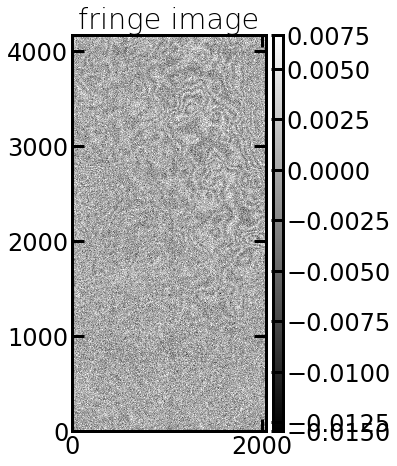
\includegraphics[width=3.70833in]{jira_imgs/3058.png}\\

}
\begin{tabular}{p{2cm}p{14cm}}
\toprule
Step 3 & Step Execution Status: \textbf{ Pass } \\ \hline
\end{tabular}
 Description \\
{\footnotesize
Apply the fringe correction to a science image and confirm that it has
the desired effect.

}
\hdashrule[0.5ex]{\textwidth}{1pt}{3mm}
  Expected Result \\
{\footnotesize
Images before and after correction have different pixel values.

}
\hdashrule[0.5ex]{\textwidth}{1pt}{3mm}
  Actual Result \\
{\footnotesize
In the attached notebook, we extracted image statistics before and after
the fringe correction, and see the following:\\[2\baselineskip]

\begin{verbatim}
  image                     median     stddev    (of image pixel values)
raw:                      17078.0 3836.131470952384
after fringe correction:  17108.0 765.4047
\end{verbatim}

We have thus demonstrated that the fringe correction has altered the
image as expected.\\[2\baselineskip]

}

\paragraph{ LVV-T126 - Verify implementation of Image Differencing }\mbox{}\\

Version \textbf{1}.
Status \textbf{Approved}.
Open  \href{https://jira.lsstcorp.org/secure/Tests.jspa#/testCase/LVV-T126}{\textit{ LVV-T126 } }
test case in Jira.

Verify that the DMS can perform image differencing from single exposures
and coadds.

\textbf{ Preconditions}:\\


Execution status: {\bf Pass }

Final comment:\\Results are in the notebook ``test\_LVV-T126.ipynb'' attached to the
Test Report repository.


Detailed steps results:

\begin{tabular}{p{2cm}p{14cm}}
\toprule
Step 1 & Step Execution Status: \textbf{ Pass } \\ \hline
\end{tabular}
 Description \\
{\footnotesize
Identify a repository containing data that have been processed through
the difference imaging pipeline. (e.g., the HiTS 2015 data that are
processed monthly for testing)

}
\hdashrule[0.5ex]{\textwidth}{1pt}{3mm}
  Expected Result \\
{\footnotesize
A dataset containing calexps, difference images, and source catalogs (of
diaSrcs).

}
\hdashrule[0.5ex]{\textwidth}{1pt}{3mm}
  Actual Result \\
{\footnotesize
We execute this test on the RSP at the IDF, using DP0.2 data and Science
Pipelines version w\_2022\_32.

}
\begin{tabular}{p{2cm}p{14cm}}
\toprule
Step 2 & Step Execution Status: \textbf{ Pass } \\ \hline
\end{tabular}
 Description \\
{\footnotesize
Identify the path to the data repository, which we will refer to as
`DATA/path', then execute the following:

}
\hdashrule[0.5ex]{\textwidth}{1pt}{3mm}
  Example Code \\
{\footnotesize
\begin{verbatim}
from lsst.daf.butler import Butler
repo = 'Data/path'
collection = 'collection'
butler = Butler(repo, collections=collection)
\end{verbatim}

}
\hdashrule[0.5ex]{\textwidth}{1pt}{3mm}
  Expected Result \\
{\footnotesize
Butler repo available for reading.

}
\hdashrule[0.5ex]{\textwidth}{1pt}{3mm}
  Actual Result \\
{\footnotesize
To instantiate the butler containing DP0.2 data:\\[2\baselineskip]config
= `dp02'\\
collection = `2.2i/runs/DP0.2'\\
butler = Butler(config, collections=collection)

}
\begin{tabular}{p{2cm}p{14cm}}
\toprule
Step 3 & Step Execution Status: \textbf{ Pass } \\ \hline
\end{tabular}
 Description \\
{\footnotesize
Extract a `calexp`, a `deepDiff\_differenceExp`, and the
`deepDiff\_diaSrc` catalog of measurements.

}
\hdashrule[0.5ex]{\textwidth}{1pt}{3mm}
  Expected Result \\
{\footnotesize
Well-formed images and catalogs containing the calexp from the visit
image and the difference image, and measurements of sources from the
difference image.

}
\hdashrule[0.5ex]{\textwidth}{1pt}{3mm}
  Actual Result \\
{\footnotesize
Select the dataId of a single visit image:\\
dataId = \{'instrument': `LSSTCam-imSim', `detector': 78, `visit':
60891, `exposure':60891, `band':'i'\}\\[2\baselineskip]Extract the
calexp image, difference image, and diaSrc catalog:\\
calexp = butler.get('calexp', dataId=dataId)\\
diffim = butler.get('goodSeeingDiff\_differenceExp', dataId=dataId)\\
diasrc = butler.get('goodSeeingDiff\_diaSrc', dataId=dataId)

}
\begin{tabular}{p{2cm}p{14cm}}
\toprule
Step 4 & Step Execution Status: \textbf{ Pass } \\ \hline
\end{tabular}
 Description \\
{\footnotesize
Confirm (by visual inspection) that the difference image is mostly blank
sky (i.e., has had a template of the same field subtracted), and that
the source catalog contains sources with photometric and astrometric
measurements.

}
\hdashrule[0.5ex]{\textwidth}{1pt}{3mm}
  Expected Result \\
{\footnotesize
A mostly blank image (with perhaps some artifacts due to imperfect
subtraction) and a catalog of sources detected/measured from that image.

}
\hdashrule[0.5ex]{\textwidth}{1pt}{3mm}
  Actual Result \\
{\footnotesize
This following figure shows the calexp image on the left and the
difference image for the same visit on the right. The difference image
contains mostly blank sky, with some minor artifacts due to imperfect
subtraction of bright
stars.\\[2\baselineskip]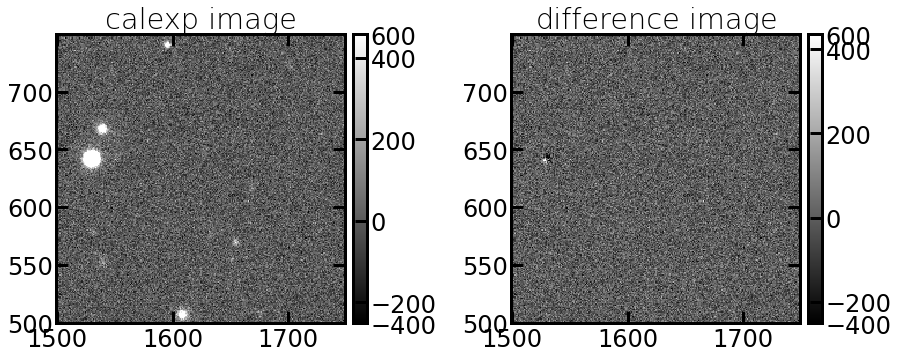
\includegraphics[width=5.90625in]{jira_imgs/3062.png}\\
The attached notebook demonstrates that the diaSrc catalog contains the
expected measurements.

}

\paragraph{ LVV-T1946 - Verify implementation of measurements in catalogs from coadds }\mbox{}\\

Version \textbf{1}.
Status \textbf{Approved}.
Open  \href{https://jira.lsstcorp.org/secure/Tests.jspa#/testCase/LVV-T1946}{\textit{ LVV-T1946 } }
test case in Jira.

Verify that source measurements in catalogs containing measurements from
coadd images are in flux units.

\textbf{ Preconditions}:\\


Execution status: {\bf Pass }

Final comment:\\Executed at the IDF using Science Pipelines version
w\_2022\_32.\\[2\baselineskip]This test case can be executed by running
the script test\_LVV-T1946.py, which is available in the test report
github repository's ``scripts/'' directory.\\[2\baselineskip]Note that
in this test we only checked source catalogs that are persisted in
butler repositories. Catalogs in other forms (e.g., parquet tables, or
tables in the Qserv database) will be confirmed separately.


Detailed steps results:

\begin{tabular}{p{2cm}p{14cm}}
\toprule
Step 1 & Step Execution Status: \textbf{ Pass } \\ \hline
\end{tabular}
 Description \\
{\footnotesize
Identify the path to the data repository, which we will refer to as
`DATA/path', then execute the following:

}
\hdashrule[0.5ex]{\textwidth}{1pt}{3mm}
  Example Code \\
{\footnotesize
\begin{verbatim}
from lsst.daf.butler import Butler
repo = 'Data/path'
collection = 'collection'
butler = Butler(repo, collections=collection)
\end{verbatim}

}
\hdashrule[0.5ex]{\textwidth}{1pt}{3mm}
  Expected Result \\
{\footnotesize
Butler repo available for reading.

}
\hdashrule[0.5ex]{\textwidth}{1pt}{3mm}
  Actual Result \\
{\footnotesize
Tests were performed by executing test\_LVV-T1946.py, which contains the
following:\\[2\baselineskip]\# For DP0.2 data on the IDF:\\
config = `dp02'\\
collection = `2.2i/runs/DP0.2'\\
butler = Butler(config, collections=collection)

}
\begin{tabular}{p{2cm}p{14cm}}
\toprule
Step 2 & Step Execution Status: \textbf{ Pass } \\ \hline
\end{tabular}
 Description \\
{\footnotesize
Identify and read an appropriate processed precursor dataset containing
coadds with the Butler.

}
\hdashrule[0.5ex]{\textwidth}{1pt}{3mm}
  Expected Result \\
{\footnotesize

}
\hdashrule[0.5ex]{\textwidth}{1pt}{3mm}
  Actual Result \\
{\footnotesize
By default, the test script contains the following tract/patch/band
combination. This can be changed if desired.\\[2\baselineskip]\# Select
an arbitrary source catalog from a deepCoadd:\\
band = `i'\\
tract = 3828\\
patch = 13\\[2\baselineskip]\# Run the test\\
LVVT1946(tract, patch, band)

}
\begin{tabular}{p{2cm}p{14cm}}
\toprule
Step 3 & Step Execution Status: \textbf{ Pass } \\ \hline
\end{tabular}
 Description \\
{\footnotesize
Verify that the coadd catalog provides measurements in flux units.

}
\hdashrule[0.5ex]{\textwidth}{1pt}{3mm}
  Expected Result \\
{\footnotesize
Confirmation of measurements in catalogs encoded in flux units.

}
\hdashrule[0.5ex]{\textwidth}{1pt}{3mm}
  Actual Result \\
{\footnotesize
Execute the script, which checks all flux fields for the input coadd
image:\\
`python test\_LVV-T1946.py`\\[2\baselineskip]Screen outputs:\\
lsst\_distrib ~ ~ ~ ~ ~g0b29ad24fb+cafeaf151e ~ ~current w\_2022\_32
setup\\
Input dataId: \{'tract': 3828, `band': `i', `patch': 13\}\\
base\_SdssShape\_instFlux \ldots{}.. count\\
base\_SdssShape\_instFluxErr \ldots{}.. count\\
base\_CircularApertureFlux\_3\_0\_instFlux \ldots{}.. count\\
base\_CircularApertureFlux\_3\_0\_instFluxErr \ldots{}.. count\\
base\_CircularApertureFlux\_4\_5\_instFlux \ldots{}.. count\\
base\_CircularApertureFlux\_4\_5\_instFluxErr \ldots{}.. count\\
base\_CircularApertureFlux\_6\_0\_instFlux \ldots{}.. count\\
base\_CircularApertureFlux\_6\_0\_instFluxErr \ldots{}.. count\\
base\_CircularApertureFlux\_9\_0\_instFlux \ldots{}.. count\\
base\_CircularApertureFlux\_9\_0\_instFluxErr \ldots{}.. count\\
base\_CircularApertureFlux\_12\_0\_instFlux \ldots{}.. count\\
base\_CircularApertureFlux\_12\_0\_instFluxErr \ldots{}.. count\\
base\_CircularApertureFlux\_17\_0\_instFlux \ldots{}.. count\\
base\_CircularApertureFlux\_17\_0\_instFluxErr \ldots{}.. count\\
base\_CircularApertureFlux\_25\_0\_instFlux \ldots{}.. count\\
base\_CircularApertureFlux\_25\_0\_instFluxErr \ldots{}.. count\\
base\_CircularApertureFlux\_35\_0\_instFlux \ldots{}.. count\\
base\_CircularApertureFlux\_35\_0\_instFluxErr \ldots{}.. count\\
base\_CircularApertureFlux\_50\_0\_instFlux \ldots{}.. count\\
base\_CircularApertureFlux\_50\_0\_instFluxErr \ldots{}.. count\\
base\_CircularApertureFlux\_70\_0\_instFlux \ldots{}.. count\\
base\_CircularApertureFlux\_70\_0\_instFluxErr \ldots{}.. count\\
base\_GaussianFlux\_instFlux \ldots{}.. count\\
base\_GaussianFlux\_instFluxErr \ldots{}.. count\\
base\_LocalBackground\_instFlux \ldots{}.. count\\
base\_LocalBackground\_instFluxErr \ldots{}.. count\\
base\_PsfFlux\_instFlux \ldots{}.. count\\
base\_PsfFlux\_instFluxErr \ldots{}.. count\\
ext\_gaap\_GaapFlux\_1\_15x\_0\_5\_instFlux \ldots{}.. count\\
ext\_gaap\_GaapFlux\_1\_15x\_0\_5\_instFluxErr \ldots{}.. count\\
ext\_gaap\_GaapFlux\_1\_15x\_0\_7\_instFlux \ldots{}.. count\\
ext\_gaap\_GaapFlux\_1\_15x\_0\_7\_instFluxErr \ldots{}.. count\\
ext\_gaap\_GaapFlux\_1\_15x\_1\_0\_instFlux \ldots{}.. count\\
ext\_gaap\_GaapFlux\_1\_15x\_1\_0\_instFluxErr \ldots{}.. count\\
ext\_gaap\_GaapFlux\_1\_15x\_1\_5\_instFlux \ldots{}.. count\\
ext\_gaap\_GaapFlux\_1\_15x\_1\_5\_instFluxErr \ldots{}.. count\\
ext\_gaap\_GaapFlux\_1\_15x\_2\_5\_instFlux \ldots{}.. count\\
ext\_gaap\_GaapFlux\_1\_15x\_2\_5\_instFluxErr \ldots{}.. count\\
ext\_gaap\_GaapFlux\_1\_15x\_3\_0\_instFlux \ldots{}.. count\\
ext\_gaap\_GaapFlux\_1\_15x\_3\_0\_instFluxErr \ldots{}.. count\\
ext\_gaap\_GaapFlux\_1\_15x\_PsfFlux\_instFlux \ldots{}.. count\\
ext\_gaap\_GaapFlux\_1\_15x\_PsfFlux\_instFluxErr \ldots{}.. count\\
ext\_gaap\_GaapFlux\_1\_15x\_Optimal\_instFlux \ldots{}.. count\\
ext\_gaap\_GaapFlux\_1\_15x\_Optimal\_instFluxErr \ldots{}.. count\\
ext\_photometryKron\_KronFlux\_instFlux \ldots{}.. count\\
ext\_photometryKron\_KronFlux\_instFluxErr \ldots{}.. count\\
ext\_convolved\_ConvolvedFlux\_0\_3\_3\_instFlux \ldots{}.. count\\
ext\_convolved\_ConvolvedFlux\_0\_3\_3\_instFluxErr \ldots{}.. count\\
ext\_convolved\_ConvolvedFlux\_0\_4\_5\_instFlux \ldots{}.. count\\
ext\_convolved\_ConvolvedFlux\_0\_4\_5\_instFluxErr \ldots{}.. count\\
ext\_convolved\_ConvolvedFlux\_0\_6\_0\_instFlux \ldots{}.. count\\
ext\_convolved\_ConvolvedFlux\_0\_6\_0\_instFluxErr \ldots{}.. count\\
ext\_convolved\_ConvolvedFlux\_0\_kron\_instFlux \ldots{}.. count\\
ext\_convolved\_ConvolvedFlux\_0\_kron\_instFluxErr \ldots{}.. count\\
ext\_convolved\_ConvolvedFlux\_1\_3\_3\_instFlux \ldots{}.. count\\
ext\_convolved\_ConvolvedFlux\_1\_3\_3\_instFluxErr \ldots{}.. count\\
ext\_convolved\_ConvolvedFlux\_1\_4\_5\_instFlux \ldots{}.. count\\
ext\_convolved\_ConvolvedFlux\_1\_4\_5\_instFluxErr \ldots{}.. count\\
ext\_convolved\_ConvolvedFlux\_1\_6\_0\_instFlux \ldots{}.. count\\
ext\_convolved\_ConvolvedFlux\_1\_6\_0\_instFluxErr \ldots{}.. count\\
ext\_convolved\_ConvolvedFlux\_1\_kron\_instFlux \ldots{}.. count\\
ext\_convolved\_ConvolvedFlux\_1\_kron\_instFluxErr \ldots{}.. count\\
ext\_convolved\_ConvolvedFlux\_2\_3\_3\_instFlux \ldots{}.. count\\
ext\_convolved\_ConvolvedFlux\_2\_3\_3\_instFluxErr \ldots{}.. count\\
ext\_convolved\_ConvolvedFlux\_2\_4\_5\_instFlux \ldots{}.. count\\
ext\_convolved\_ConvolvedFlux\_2\_4\_5\_instFluxErr \ldots{}.. count\\
ext\_convolved\_ConvolvedFlux\_2\_6\_0\_instFlux \ldots{}.. count\\
ext\_convolved\_ConvolvedFlux\_2\_6\_0\_instFluxErr \ldots{}.. count\\
ext\_convolved\_ConvolvedFlux\_2\_kron\_instFlux \ldots{}.. count\\
ext\_convolved\_ConvolvedFlux\_2\_kron\_instFluxErr \ldots{}.. count\\
ext\_convolved\_ConvolvedFlux\_3\_3\_3\_instFlux \ldots{}.. count\\
ext\_convolved\_ConvolvedFlux\_3\_3\_3\_instFluxErr \ldots{}.. count\\
ext\_convolved\_ConvolvedFlux\_3\_4\_5\_instFlux \ldots{}.. count\\
ext\_convolved\_ConvolvedFlux\_3\_4\_5\_instFluxErr \ldots{}.. count\\
ext\_convolved\_ConvolvedFlux\_3\_6\_0\_instFlux \ldots{}.. count\\
ext\_convolved\_ConvolvedFlux\_3\_6\_0\_instFluxErr \ldots{}.. count\\
ext\_convolved\_ConvolvedFlux\_3\_kron\_instFlux \ldots{}.. count\\
ext\_convolved\_ConvolvedFlux\_3\_kron\_instFluxErr \ldots{}.. count\\
modelfit\_CModel\_initial\_instFlux \ldots{}.. count\\
modelfit\_CModel\_initial\_instFluxErr \ldots{}.. count\\
modelfit\_CModel\_initial\_instFlux\_inner \ldots{}.. count\\
modelfit\_CModel\_exp\_instFlux \ldots{}.. count\\
modelfit\_CModel\_exp\_instFluxErr \ldots{}.. count\\
modelfit\_CModel\_exp\_instFlux\_inner \ldots{}.. count\\
modelfit\_CModel\_dev\_instFlux \ldots{}.. count\\
modelfit\_CModel\_dev\_instFluxErr \ldots{}.. count\\
modelfit\_CModel\_dev\_instFlux\_inner \ldots{}.. count\\
modelfit\_CModel\_instFlux \ldots{}.. count\\
modelfit\_CModel\_instFluxErr \ldots{}.. count\\
modelfit\_CModel\_instFlux\_inner \ldots{}.. count\\
undeblended\_base\_CircularApertureFlux\_3\_0\_instFlux \ldots{}..
count\\
undeblended\_base\_CircularApertureFlux\_3\_0\_instFluxErr \ldots{}..
count\\
undeblended\_base\_CircularApertureFlux\_4\_5\_instFlux \ldots{}..
count\\
undeblended\_base\_CircularApertureFlux\_4\_5\_instFluxErr \ldots{}..
count\\
undeblended\_base\_CircularApertureFlux\_6\_0\_instFlux \ldots{}..
count\\
undeblended\_base\_CircularApertureFlux\_6\_0\_instFluxErr \ldots{}..
count\\
undeblended\_base\_CircularApertureFlux\_9\_0\_instFlux \ldots{}..
count\\
undeblended\_base\_CircularApertureFlux\_9\_0\_instFluxErr \ldots{}..
count\\
undeblended\_base\_CircularApertureFlux\_12\_0\_instFlux \ldots{}..
count\\
undeblended\_base\_CircularApertureFlux\_12\_0\_instFluxErr \ldots{}..
count\\
undeblended\_base\_CircularApertureFlux\_17\_0\_instFlux \ldots{}..
count\\
undeblended\_base\_CircularApertureFlux\_17\_0\_instFluxErr \ldots{}..
count\\
undeblended\_base\_CircularApertureFlux\_25\_0\_instFlux \ldots{}..
count\\
undeblended\_base\_CircularApertureFlux\_25\_0\_instFluxErr \ldots{}..
count\\
undeblended\_base\_CircularApertureFlux\_35\_0\_instFlux \ldots{}..
count\\
undeblended\_base\_CircularApertureFlux\_35\_0\_instFluxErr \ldots{}..
count\\
undeblended\_base\_CircularApertureFlux\_50\_0\_instFlux \ldots{}..
count\\
undeblended\_base\_CircularApertureFlux\_50\_0\_instFluxErr \ldots{}..
count\\
undeblended\_base\_CircularApertureFlux\_70\_0\_instFlux \ldots{}..
count\\
undeblended\_base\_CircularApertureFlux\_70\_0\_instFluxErr \ldots{}..
count\\
undeblended\_base\_PsfFlux\_instFlux \ldots{}.. count\\
undeblended\_base\_PsfFlux\_instFluxErr \ldots{}.. count\\
undeblended\_ext\_gaap\_GaapFlux\_1\_15x\_0\_5\_instFlux \ldots{}..
count\\
undeblended\_ext\_gaap\_GaapFlux\_1\_15x\_0\_5\_instFluxErr \ldots{}..
count\\
undeblended\_ext\_gaap\_GaapFlux\_1\_15x\_0\_7\_instFlux \ldots{}..
count\\
undeblended\_ext\_gaap\_GaapFlux\_1\_15x\_0\_7\_instFluxErr \ldots{}..
count\\
undeblended\_ext\_gaap\_GaapFlux\_1\_15x\_1\_0\_instFlux \ldots{}..
count\\
undeblended\_ext\_gaap\_GaapFlux\_1\_15x\_1\_0\_instFluxErr \ldots{}..
count\\
undeblended\_ext\_gaap\_GaapFlux\_1\_15x\_1\_5\_instFlux \ldots{}..
count\\
undeblended\_ext\_gaap\_GaapFlux\_1\_15x\_1\_5\_instFluxErr \ldots{}..
count\\
undeblended\_ext\_gaap\_GaapFlux\_1\_15x\_2\_5\_instFlux \ldots{}..
count\\
undeblended\_ext\_gaap\_GaapFlux\_1\_15x\_2\_5\_instFluxErr \ldots{}..
count\\
undeblended\_ext\_gaap\_GaapFlux\_1\_15x\_3\_0\_instFlux \ldots{}..
count\\
undeblended\_ext\_gaap\_GaapFlux\_1\_15x\_3\_0\_instFluxErr \ldots{}..
count\\
undeblended\_ext\_gaap\_GaapFlux\_1\_15x\_PsfFlux\_instFlux \ldots{}..
count\\
undeblended\_ext\_gaap\_GaapFlux\_1\_15x\_PsfFlux\_instFluxErr
\ldots{}.. count\\
undeblended\_ext\_gaap\_GaapFlux\_1\_15x\_Optimal\_instFlux \ldots{}..
count\\
undeblended\_ext\_gaap\_GaapFlux\_1\_15x\_Optimal\_instFluxErr
\ldots{}.. count\\
undeblended\_ext\_photometryKron\_KronFlux\_instFlux \ldots{}.. count\\
undeblended\_ext\_photometryKron\_KronFlux\_instFluxErr \ldots{}..
count\\
undeblended\_ext\_convolved\_ConvolvedFlux\_0\_3\_3\_instFlux \ldots{}..
count\\
undeblended\_ext\_convolved\_ConvolvedFlux\_0\_3\_3\_instFluxErr
\ldots{}.. count\\
undeblended\_ext\_convolved\_ConvolvedFlux\_0\_4\_5\_instFlux \ldots{}..
count\\
undeblended\_ext\_convolved\_ConvolvedFlux\_0\_4\_5\_instFluxErr
\ldots{}.. count\\
undeblended\_ext\_convolved\_ConvolvedFlux\_0\_6\_0\_instFlux \ldots{}..
count\\
undeblended\_ext\_convolved\_ConvolvedFlux\_0\_6\_0\_instFluxErr
\ldots{}.. count\\
undeblended\_ext\_convolved\_ConvolvedFlux\_0\_kron\_instFlux \ldots{}..
count\\
undeblended\_ext\_convolved\_ConvolvedFlux\_0\_kron\_instFluxErr
\ldots{}.. count\\
undeblended\_ext\_convolved\_ConvolvedFlux\_1\_3\_3\_instFlux \ldots{}..
count\\
undeblended\_ext\_convolved\_ConvolvedFlux\_1\_3\_3\_instFluxErr
\ldots{}.. count\\
undeblended\_ext\_convolved\_ConvolvedFlux\_1\_4\_5\_instFlux \ldots{}..
count\\
undeblended\_ext\_convolved\_ConvolvedFlux\_1\_4\_5\_instFluxErr
\ldots{}.. count\\
undeblended\_ext\_convolved\_ConvolvedFlux\_1\_6\_0\_instFlux \ldots{}..
count\\
undeblended\_ext\_convolved\_ConvolvedFlux\_1\_6\_0\_instFluxErr
\ldots{}.. count\\
undeblended\_ext\_convolved\_ConvolvedFlux\_1\_kron\_instFlux \ldots{}..
count\\
undeblended\_ext\_convolved\_ConvolvedFlux\_1\_kron\_instFluxErr
\ldots{}.. count\\
undeblended\_ext\_convolved\_ConvolvedFlux\_2\_3\_3\_instFlux \ldots{}..
count\\
undeblended\_ext\_convolved\_ConvolvedFlux\_2\_3\_3\_instFluxErr
\ldots{}.. count\\
undeblended\_ext\_convolved\_ConvolvedFlux\_2\_4\_5\_instFlux \ldots{}..
count\\
undeblended\_ext\_convolved\_ConvolvedFlux\_2\_4\_5\_instFluxErr
\ldots{}.. count\\
undeblended\_ext\_convolved\_ConvolvedFlux\_2\_6\_0\_instFlux \ldots{}..
count\\
undeblended\_ext\_convolved\_ConvolvedFlux\_2\_6\_0\_instFluxErr
\ldots{}.. count\\
undeblended\_ext\_convolved\_ConvolvedFlux\_2\_kron\_instFlux \ldots{}..
count\\
undeblended\_ext\_convolved\_ConvolvedFlux\_2\_kron\_instFluxErr
\ldots{}.. count\\
undeblended\_ext\_convolved\_ConvolvedFlux\_3\_3\_3\_instFlux \ldots{}..
count\\
undeblended\_ext\_convolved\_ConvolvedFlux\_3\_3\_3\_instFluxErr
\ldots{}.. count\\
undeblended\_ext\_convolved\_ConvolvedFlux\_3\_4\_5\_instFlux \ldots{}..
count\\
undeblended\_ext\_convolved\_ConvolvedFlux\_3\_4\_5\_instFluxErr
\ldots{}.. count\\
undeblended\_ext\_convolved\_ConvolvedFlux\_3\_6\_0\_instFlux \ldots{}..
count\\
undeblended\_ext\_convolved\_ConvolvedFlux\_3\_6\_0\_instFluxErr
\ldots{}.. count\\
undeblended\_ext\_convolved\_ConvolvedFlux\_3\_kron\_instFlux \ldots{}..
count\\
undeblended\_ext\_convolved\_ConvolvedFlux\_3\_kron\_instFluxErr
\ldots{}.. count\\[2\baselineskip]All forced\_src instFlux entries have
units of counts: True\\[2\baselineskip]All flux fields have units of
``counts'', so this test has passed.

}

\paragraph{ LVV-T1947 - Verify implementation of measurements in catalogs from difference images }\mbox{}\\

Version \textbf{1}.
Status \textbf{Approved}.
Open  \href{https://jira.lsstcorp.org/secure/Tests.jspa#/testCase/LVV-T1947}{\textit{ LVV-T1947 } }
test case in Jira.

Verify that source measurements in catalogs containing measurements from
difference images are in flux units.

\textbf{ Preconditions}:\\


Execution status: {\bf Pass }

Final comment:\\Executed at the IDF using Science Pipelines version
w\_2022\_32.\\[2\baselineskip]This test case can be executed by running
the script test\_LVV-T1947.py, which is available in the test report
github repository's ``scripts/'' directory.\\[2\baselineskip]Note that
in this test we only checked source catalogs that are persisted in
butler repositories. Catalogs in other forms (e.g., parquet tables, or
tables in the Qserv database) will be confirmed separately.


Detailed steps results:

\begin{tabular}{p{2cm}p{14cm}}
\toprule
Step 1 & Step Execution Status: \textbf{ Pass } \\ \hline
\end{tabular}
 Description \\
{\footnotesize
Identify the path to the data repository, which we will refer to as
`DATA/path', then execute the following:

}
\hdashrule[0.5ex]{\textwidth}{1pt}{3mm}
  Example Code \\
{\footnotesize
\begin{verbatim}
from lsst.daf.butler import Butler
repo = 'Data/path'
collection = 'collection'
butler = Butler(repo, collections=collection)
\end{verbatim}

}
\hdashrule[0.5ex]{\textwidth}{1pt}{3mm}
  Expected Result \\
{\footnotesize
Butler repo available for reading.

}
\hdashrule[0.5ex]{\textwidth}{1pt}{3mm}
  Actual Result \\
{\footnotesize
Tests were performed by executing test\_LVV-T1947.py, which contains the
following:\\[2\baselineskip]\# For DP0.2 data on the IDF:\\
config = `dp02'\\
collection = `2.2i/runs/DP0.2'\\
butler = Butler(config, collections=collection)

}
\begin{tabular}{p{2cm}p{14cm}}
\toprule
Step 2 & Step Execution Status: \textbf{ Pass } \\ \hline
\end{tabular}
 Description \\
{\footnotesize
Identify and read an appropriate processed precursor dataset containing
difference images with the Butler.

}
\hdashrule[0.5ex]{\textwidth}{1pt}{3mm}
  Expected Result \\
{\footnotesize

}
\hdashrule[0.5ex]{\textwidth}{1pt}{3mm}
  Actual Result \\
{\footnotesize
By default, the test script contains the following tract/patch/band
combination. This can be changed if desired.\\[2\baselineskip]\# Select
an arbitrary source catalog from a difference image:\\
instrument = `LSSTCam-imSim'\\
detector = 5\\
visit = 924041\\[2\baselineskip]\# Run the test\\
LVVT1947(instrument, visit, detector)

}
\begin{tabular}{p{2cm}p{14cm}}
\toprule
Step 3 & Step Execution Status: \textbf{ Pass } \\ \hline
\end{tabular}
 Description \\
{\footnotesize
Verify that the difference image source catalog provides measurements in
flux units.

}
\hdashrule[0.5ex]{\textwidth}{1pt}{3mm}
  Expected Result \\
{\footnotesize
Confirmation of measurements in catalogs encoded in flux units.

}
\hdashrule[0.5ex]{\textwidth}{1pt}{3mm}
  Actual Result \\
{\footnotesize
Execute the script, which checks all flux fields for the input
goodSeeingDiff image:\\
`python test\_LVV-T1947.py`\\[2\baselineskip]Screen
outputs:\\[2\baselineskip]lsst\_distrib ~ ~ ~ ~ ~g0b29ad24fb+cafeaf151e
~ ~current w\_2022\_32 setup\\
Input dataId: \{'instrument': `LSSTCam-imSim', `visit': 924041,
`detector': 5\}\\
base\_SdssShape\_instFlux \ldots{}.. count\\
base\_SdssShape\_instFluxErr \ldots{}.. count\\
base\_CircularApertureFlux\_3\_0\_instFlux \ldots{}.. count\\
base\_CircularApertureFlux\_3\_0\_instFluxErr \ldots{}.. count\\
base\_CircularApertureFlux\_4\_5\_instFlux \ldots{}.. count\\
base\_CircularApertureFlux\_4\_5\_instFluxErr \ldots{}.. count\\
base\_CircularApertureFlux\_6\_0\_instFlux \ldots{}.. count\\
base\_CircularApertureFlux\_6\_0\_instFluxErr \ldots{}.. count\\
base\_CircularApertureFlux\_9\_0\_instFlux \ldots{}.. count\\
base\_CircularApertureFlux\_9\_0\_instFluxErr \ldots{}.. count\\
base\_CircularApertureFlux\_12\_0\_instFlux \ldots{}.. count\\
base\_CircularApertureFlux\_12\_0\_instFluxErr \ldots{}.. count\\
base\_CircularApertureFlux\_17\_0\_instFlux \ldots{}.. count\\
base\_CircularApertureFlux\_17\_0\_instFluxErr \ldots{}.. count\\
base\_CircularApertureFlux\_25\_0\_instFlux \ldots{}.. count\\
base\_CircularApertureFlux\_25\_0\_instFluxErr \ldots{}.. count\\
base\_CircularApertureFlux\_35\_0\_instFlux \ldots{}.. count\\
base\_CircularApertureFlux\_35\_0\_instFluxErr \ldots{}.. count\\
base\_CircularApertureFlux\_50\_0\_instFlux \ldots{}.. count\\
base\_CircularApertureFlux\_50\_0\_instFluxErr \ldots{}.. count\\
base\_CircularApertureFlux\_70\_0\_instFlux \ldots{}.. count\\
base\_CircularApertureFlux\_70\_0\_instFluxErr \ldots{}.. count\\
base\_GaussianFlux\_instFlux \ldots{}.. count\\
base\_GaussianFlux\_instFluxErr \ldots{}.. count\\
base\_PeakLikelihoodFlux\_instFlux \ldots{}.. count\\
base\_PeakLikelihoodFlux\_instFluxErr \ldots{}.. count\\
base\_PsfFlux\_instFlux \ldots{}.. count\\
base\_PsfFlux\_instFluxErr \ldots{}.. count\\
ip\_diffim\_NaiveDipoleFlux\_pos\_instFlux \ldots{}.. count\\
ip\_diffim\_NaiveDipoleFlux\_pos\_instFluxErr \ldots{}.. count\\
ip\_diffim\_NaiveDipoleFlux\_neg\_instFlux \ldots{}.. count\\
ip\_diffim\_NaiveDipoleFlux\_neg\_instFluxErr \ldots{}.. count\\
ip\_diffim\_PsfDipoleFlux\_pos\_instFlux \ldots{}.. count\\
ip\_diffim\_PsfDipoleFlux\_pos\_instFluxErr \ldots{}.. count\\
ip\_diffim\_PsfDipoleFlux\_neg\_instFlux \ldots{}.. count\\
ip\_diffim\_PsfDipoleFlux\_neg\_instFluxErr \ldots{}.. count\\
ip\_diffim\_DipoleFit\_pos\_instFlux \ldots{}.. count\\
ip\_diffim\_DipoleFit\_pos\_instFluxErr \ldots{}.. count\\
ip\_diffim\_DipoleFit\_neg\_instFlux \ldots{}.. count\\
ip\_diffim\_DipoleFit\_neg\_instFluxErr \ldots{}.. count\\
ip\_diffim\_DipoleFit\_instFlux \ldots{}.. count\\
ip\_diffim\_forced\_PsfFlux\_instFlux \ldots{}.. count\\
ip\_diffim\_forced\_PsfFlux\_instFluxErr \ldots{}..
count\\[2\baselineskip]All diaSrc table instFlux entries have units of
counts: True\\[2\baselineskip]All flux fields have units of ``counts'',
so this test has passed.

}

\paragraph{ LVV-T28 - Verify implementation of measurements in catalogs from PVIs }\mbox{}\\

Version \textbf{1}.
Status \textbf{Approved}.
Open  \href{https://jira.lsstcorp.org/secure/Tests.jspa#/testCase/LVV-T28}{\textit{ LVV-T28 } }
test case in Jira.

Verify that source measurements in catalogs containing measurements from
processed visit images are in flux units.

\textbf{ Preconditions}:\\


Execution status: {\bf Pass }

Final comment:\\Executed at the IDF using Science Pipelines version
w\_2022\_32.\\[2\baselineskip]This test case can be executed by running
the script test\_LVV-T28.py, which is available in the test report
github repository's ``scripts/'' directory.\\[2\baselineskip]Note that
in this test we only checked source catalogs that are persisted in
butler repositories. Catalogs in other forms (e.g., parquet tables, or
tables in the Qserv database) will be confirmed separately.


Detailed steps results:

\begin{tabular}{p{2cm}p{14cm}}
\toprule
Step 1 & Step Execution Status: \textbf{ Pass } \\ \hline
\end{tabular}
 Description \\
{\footnotesize
Identify the path to the data repository, which we will refer to as
`DATA/path', then execute the following:

}
\hdashrule[0.5ex]{\textwidth}{1pt}{3mm}
  Example Code \\
{\footnotesize
\begin{verbatim}
from lsst.daf.butler import Butler
repo = 'Data/path'
collection = 'collection'
butler = Butler(repo, collections=collection)
\end{verbatim}

}
\hdashrule[0.5ex]{\textwidth}{1pt}{3mm}
  Expected Result \\
{\footnotesize
Butler repo available for reading.

}
\hdashrule[0.5ex]{\textwidth}{1pt}{3mm}
  Actual Result \\
{\footnotesize
Tests were performed by executing test\_LVV-T28.py, which contains the
following:\\[2\baselineskip]\# For DP0.2 data on the IDF:\\
config = `dp02'\\
collection = `2.2i/runs/DP0.2'\\
butler = Butler(config, collections=collection)

}
\begin{tabular}{p{2cm}p{14cm}}
\toprule
Step 2 & Step Execution Status: \textbf{ Pass } \\ \hline
\end{tabular}
 Description \\
{\footnotesize
Identify and read an appropriate processed precursor dataset containing
coadds with the Butler.~

}
\hdashrule[0.5ex]{\textwidth}{1pt}{3mm}
  Expected Result \\
{\footnotesize

}
\hdashrule[0.5ex]{\textwidth}{1pt}{3mm}
  Actual Result \\
{\footnotesize
By default, the test script contains the following tract/patch/band
combination. This can be changed if desired.\\[2\baselineskip]\# Select
an arbitrary source catalog from a deepCoadd:\\
instrument = `LSSTCam-imSim'\\
detector = 5\\
visit = 924041\\[2\baselineskip]\# Run the test\\
LVVT28(instrument, visit, detector)

}
\begin{tabular}{p{2cm}p{14cm}}
\toprule
Step 3 & Step Execution Status: \textbf{ Pass } \\ \hline
\end{tabular}
 Description \\
{\footnotesize
Verify that the single-visit catalog provides measurements in flux
units.

}
\hdashrule[0.5ex]{\textwidth}{1pt}{3mm}
  Expected Result \\
{\footnotesize
Confirmation of measurements in catalogs encoded in flux units.

}
\hdashrule[0.5ex]{\textwidth}{1pt}{3mm}
  Actual Result \\
{\footnotesize
Execute the script, which checks all flux fields for the input PVI:\\
`python test\_LVV-T28.py`\\[2\baselineskip]lsst\_distrib ~ ~ ~ ~
~g0b29ad24fb+cafeaf151e ~ ~current w\_2022\_32 setup\\
Input dataId: \{'instrument': `LSSTCam-imSim', `visit': 924041,
`detector': 5\}\\
deblend\_psf\_instFlux \ldots{}.. count\\
base\_Blendedness\_raw\_child\_instFlux \ldots{}.. count\\
base\_Blendedness\_raw\_parent\_instFlux \ldots{}.. count\\
base\_Blendedness\_abs\_child\_instFlux \ldots{}.. count\\
base\_Blendedness\_abs\_parent\_instFlux \ldots{}.. count\\
base\_SdssShape\_instFlux \ldots{}.. count\\
base\_SdssShape\_instFluxErr \ldots{}.. count\\
base\_CircularApertureFlux\_3\_0\_instFlux \ldots{}.. count\\
base\_CircularApertureFlux\_3\_0\_instFluxErr \ldots{}.. count\\
base\_CircularApertureFlux\_4\_5\_instFlux \ldots{}.. count\\
base\_CircularApertureFlux\_4\_5\_instFluxErr \ldots{}.. count\\
base\_CircularApertureFlux\_6\_0\_instFlux \ldots{}.. count\\
base\_CircularApertureFlux\_6\_0\_instFluxErr \ldots{}.. count\\
base\_CircularApertureFlux\_9\_0\_instFlux \ldots{}.. count\\
base\_CircularApertureFlux\_9\_0\_instFluxErr \ldots{}.. count\\
base\_CircularApertureFlux\_12\_0\_instFlux \ldots{}.. count\\
base\_CircularApertureFlux\_12\_0\_instFluxErr \ldots{}.. count\\
base\_CircularApertureFlux\_17\_0\_instFlux \ldots{}.. count\\
base\_CircularApertureFlux\_17\_0\_instFluxErr \ldots{}.. count\\
base\_CircularApertureFlux\_25\_0\_instFlux \ldots{}.. count\\
base\_CircularApertureFlux\_25\_0\_instFluxErr \ldots{}.. count\\
base\_CircularApertureFlux\_35\_0\_instFlux \ldots{}.. count\\
base\_CircularApertureFlux\_35\_0\_instFluxErr \ldots{}.. count\\
base\_CircularApertureFlux\_50\_0\_instFlux \ldots{}.. count\\
base\_CircularApertureFlux\_50\_0\_instFluxErr \ldots{}.. count\\
base\_CircularApertureFlux\_70\_0\_instFlux \ldots{}.. count\\
base\_CircularApertureFlux\_70\_0\_instFluxErr \ldots{}.. count\\
base\_GaussianFlux\_instFlux \ldots{}.. count\\
base\_GaussianFlux\_instFluxErr \ldots{}.. count\\
base\_LocalBackground\_instFlux \ldots{}.. count\\
base\_LocalBackground\_instFluxErr \ldots{}.. count\\
base\_PsfFlux\_instFlux \ldots{}.. count\\
base\_PsfFlux\_instFluxErr \ldots{}.. count\\
ext\_photometryKron\_KronFlux\_instFlux \ldots{}.. count\\
ext\_photometryKron\_KronFlux\_instFluxErr \ldots{}..
count\\[2\baselineskip]All src table instFlux entries have units of
counts: True\\[2\baselineskip]All flux fields have units of ``counts'',
so this test has passed.

}

\paragraph{ LVV-T78 - Verify implementation of Persisting Data Products }\mbox{}\\

Version \textbf{1}.
Status \textbf{Approved}.
Open  \href{https://jira.lsstcorp.org/secure/Tests.jspa#/testCase/LVV-T78}{\textit{ LVV-T78 } }
test case in Jira.

Verify that per-band deep coadds and best-seeing coadds are present,
kept, and available.

\textbf{ Preconditions}:\\
Precursor data from HSC PDR or simulated DC2 data (as reprocessed with
LSST Science Pipelines to produce Data Preview 0.2).

Execution status: {\bf Pass }

Final comment:\\The python test script to execute this code is attached to the Test
Report github repository in scripts/test\_LVV-T78.py.


Detailed steps results:

\begin{tabular}{p{2cm}p{14cm}}
\toprule
Step 1 & Step Execution Status: \textbf{ Pass } \\ \hline
\end{tabular}
 Description \\
{\footnotesize
Identify the path to the data repository, which we will refer to as
`DATA/path', then execute the following:

}
\hdashrule[0.5ex]{\textwidth}{1pt}{3mm}
  Example Code \\
{\footnotesize
\begin{verbatim}
from lsst.daf.butler import Butler
repo = 'Data/path'
collection = 'collection'
butler = Butler(repo, collections=collection)
\end{verbatim}

}
\hdashrule[0.5ex]{\textwidth}{1pt}{3mm}
  Expected Result \\
{\footnotesize
Butler repo available for reading.

}
\hdashrule[0.5ex]{\textwidth}{1pt}{3mm}
  Actual Result \\
{\footnotesize
Test executed on the RSP at the IDF. The test script confirms the
pipelines version by printing the following to the
screen:\\[2\baselineskip]lsst\_distrib g0b29ad24fb+cafeaf151e current
w\_2022\_32 setup

}
\begin{tabular}{p{2cm}p{14cm}}
\toprule
Step 2 & Step Execution Status: \textbf{ Pass } \\ \hline
\end{tabular}
 Description \\
{\footnotesize
Identify some single-band deep coadds and retrieve them from the butler

}
\hdashrule[0.5ex]{\textwidth}{1pt}{3mm}
  Expected Result \\
{\footnotesize

}
\hdashrule[0.5ex]{\textwidth}{1pt}{3mm}
  Actual Result \\
{\footnotesize
We use the DP0.2 data via the following:\\[2\baselineskip]config =
`dp02'\\
collection = `2.2i/runs/DP0.2'\\
butler = Butler(config, collections=collection)

}
\begin{tabular}{p{2cm}p{14cm}}
\toprule
Step 3 & Step Execution Status: \textbf{ Pass } \\ \hline
\end{tabular}
 Description \\
{\footnotesize
Examine the deep coadds and confirm that they are well-formed images

}
\hdashrule[0.5ex]{\textwidth}{1pt}{3mm}
  Expected Result \\
{\footnotesize

}
\hdashrule[0.5ex]{\textwidth}{1pt}{3mm}
  Actual Result \\
{\footnotesize
All subsequent steps were executed as part of the python script
test\_LVV-T78.py. The results are posted below.

}
\begin{tabular}{p{2cm}p{14cm}}
\toprule
Step 4 & Step Execution Status: \textbf{ Pass } \\ \hline
\end{tabular}
 Description \\
{\footnotesize
Identify some single-band best-seeing coadds and retrieve them from the
butler

}
\hdashrule[0.5ex]{\textwidth}{1pt}{3mm}
  Expected Result \\
{\footnotesize

}
\hdashrule[0.5ex]{\textwidth}{1pt}{3mm}
  Actual Result \\
{\footnotesize

}
\begin{tabular}{p{2cm}p{14cm}}
\toprule
Step 5 & Step Execution Status: \textbf{ Pass } \\ \hline
\end{tabular}
 Description \\
{\footnotesize
Examine the best-seeing coadds and confirm that they are well-formed
images

}
\hdashrule[0.5ex]{\textwidth}{1pt}{3mm}
  Expected Result \\
{\footnotesize

}
\hdashrule[0.5ex]{\textwidth}{1pt}{3mm}
  Actual Result \\
{\footnotesize
The output of the python script is as follows. This script reads both a
best-seeing coadd and a deep coadd corresponding to the same dataId,
prints statistics of each image to the screen, examines the variance
plane and mask to confirm they are well-formed, and confirms that each
image has an associated PSF and WCS.\\[2\baselineskip]Input dataId:
\{'tract': 4431, `patch': 17, `band': `u'\}\\[2\baselineskip]Best-seeing
coadd image shape and statistics:\\
Shape: (4200, 4200)\\
Mean, median, std deviation of pixel values: 0.03438813 0.0024560345
5.8153605\\[2\baselineskip]Deep coadd image shape and statistics:\\
Shape: (4200, 4200)\\
Mean, median, std deviation of pixel values: 0.04503397 0.0047773793
7.005774\\[2\baselineskip]Best-seeing coadd variance plane shape and
statistics:\\
Shape: (4200, 4200)\\
Mean, median, std deviation of pixel values: 0.020518279 0.019447705
0.10152267\\[2\baselineskip]Deep coadd variance plane shape and
statistics:\\
Shape: (4200, 4200)\\
Mean, median, std deviation of pixel values: 0.0056145624 0.0053308182
0.14121237\\
Best-seeing coadd mask plane has dimensions: (4200, 4200)\\
Deep coadd mask plane has dimensions: (4200, 4200)\\
Both images have a WCS.\\
Both images have a PSF.\\[2\baselineskip]Input dataId: \{'tract': 4431,
`patch': 17, `band': `g'\}\\[2\baselineskip]Best-seeing coadd image
shape and statistics:\\
Shape: (4200, 4200)\\
Mean, median, std deviation of pixel values: 0.041773453 0.002788621
2.0373423\\[2\baselineskip]Deep coadd image shape and statistics:\\
Shape: (4200, 4200)\\
Mean, median, std deviation of pixel values: 0.05321344 0.0066212164
2.2148554\\[2\baselineskip]Best-seeing coadd variance plane shape and
statistics:\\
Shape: (4200, 4200)\\
Mean, median, std deviation of pixel values: 0.002616897 0.002469438
0.0104264915\\[2\baselineskip]Deep coadd variance plane shape and
statistics:\\
Shape: (4200, 4200)\\
Mean, median, std deviation of pixel values: 0.00074665045 0.00070681534
0.0032021273\\
Best-seeing coadd mask plane has dimensions: (4200, 4200)\\
Deep coadd mask plane has dimensions: (4200, 4200)\\
Both images have a WCS.\\
Both images have a PSF.\\[2\baselineskip]Input dataId: \{'tract': 4431,
`patch': 17, `band': `r'\}\\[2\baselineskip]Best-seeing coadd image
shape and statistics:\\
Shape: (4200, 4200)\\
Mean, median, std deviation of pixel values: 0.08445272 0.0020215698
2.8918285\\[2\baselineskip]Deep coadd image shape and statistics:\\
Shape: (4200, 4200)\\
Mean, median, std deviation of pixel values: 0.10712123 0.009368613
3.528262\\[2\baselineskip]Best-seeing coadd variance plane shape and
statistics:\\
Shape: (4200, 4200)\\
Mean, median, std deviation of pixel values: 0.002568767 0.0024733383
0.011166171\\[2\baselineskip]Deep coadd variance plane shape and
statistics:\\
Shape: (4200, 4200)\\
Mean, median, std deviation of pixel values: 0.00093781634 0.0008518264
0.012951709\\
Best-seeing coadd mask plane has dimensions: (4200, 4200)\\
Deep coadd mask plane has dimensions: (4200, 4200)\\
Both images have a WCS.\\
Both images have a PSF.\\[2\baselineskip]Input dataId: ~\{'tract': 4431,
`patch': 17, `band': `i'\}\\[2\baselineskip]Best-seeing coadd image
shape and statistics:\\
Shape: (4200, 4200)\\
Mean, median, std deviation of pixel values: 0.12454637 0.0037209666
4.126306\\[2\baselineskip]Deep coadd image shape and statistics:\\
Shape: (4200, 4200)\\
Mean, median, std deviation of pixel values: 0.15418924 0.0157091
4.6056767\\[2\baselineskip]Best-seeing coadd variance plane shape and
statistics:\\
Shape: (4200, 4200)\\
Mean, median, std deviation of pixel values: inf 0.009205212
nan\\[2\baselineskip]Deep coadd variance plane shape and statistics:\\
Shape: (4200, 4200)\\
Mean, median, std deviation of pixel values: inf 0.0031147646 nan\\
Best-seeing coadd mask plane has dimensions: (4200, 4200)\\
Deep coadd mask plane has dimensions: (4200, 4200)\\
Both images have a WCS.\\
Both images have a PSF.\\[2\baselineskip]Input dataId: \{'tract': 4431,
`patch': 17, `band': `z'\}\\[2\baselineskip]Best-seeing coadd image
shape and statistics:\\
Shape: (4200, 4200)\\
Mean, median, std deviation of pixel values: 0.15889181 0.012767363
5.4510126\\[2\baselineskip]Deep coadd image shape and statistics:\\
Shape: (4200, 4200)\\
Mean, median, std deviation of pixel values: 0.18890294 0.026478318
5.2928886\\[2\baselineskip]Best-seeing coadd variance plane shape and
statistics:\\
Shape: (4200, 4200)\\
Mean, median, std deviation of pixel values: ~0.082706526 0.080273375
0.040728822\\[2\baselineskip]Deep coadd variance plane shape and
statistics:\\
Shape: (4200, 4200)\\
Mean, median, std deviation of pixel values: 0.026652763 0.026110252
0.019691393\\
Best-seeing coadd mask plane has dimensions: (4200, 4200)\\
Deep coadd mask plane has dimensions: (4200, 4200)\\
Both images have a WCS.\\
Both images have a PSF.\\[2\baselineskip]Input dataId: \{'tract': 4431,
`patch': 17, `band': `y'\}\\[2\baselineskip]Best-seeing coadd image
shape and statistics:\\
Shape: (4200, 4200)\\
Mean, median, std deviation of pixel values: 0.2097747 0.022823093
7.169966\\[2\baselineskip]Deep coadd image shape and statistics:\\
Shape: (4200, 4200)\\
Mean, median, std deviation of pixel values: 0.26832125 0.039412603
10.62081\\[2\baselineskip]Best-seeing coadd variance plane shape and
statistics:\\
Shape: (4200, 4200)\\
Mean, median, std deviation of pixel values: 0.26777592 0.26288232
0.16389878\\[2\baselineskip]Deep coadd variance plane shape and
statistics:\\
Shape: (4200, 4200)\\
Mean, median, std deviation of pixel values: 0.08693949 0.08555089
0.26010248\\
Best-seeing coadd mask plane has dimensions: (4200, 4200)\\
Deep coadd mask plane has dimensions: (4200, 4200)\\
Both images have a WCS.\\
Both images have a PSF.\\[2\baselineskip]We have thus verified that deep
and best-seeing coadds are present, retained, and available, and are
well-formed.

}

\paragraph{ LVV-T42 - Verify implementation of Processed Visit Image Content }\mbox{}\\

Version \textbf{1}.
Status \textbf{Approved}.
Open  \href{https://jira.lsstcorp.org/secure/Tests.jspa#/testCase/LVV-T42}{\textit{ LVV-T42 } }
test case in Jira.

Verify that Processed Visit Images produced by the DRP and AP pipelines
include the observed data, a mask array, a variance array, a PSF model,
and a WCS model.

\textbf{ Preconditions}:\\


Execution status: {\bf Pass }

Final comment:\\Results are in the notebook ``test\_LVV-T42.ipynb'' attached to the Test
Report repository.


Detailed steps results:

\begin{tabular}{p{2cm}p{14cm}}
\toprule
Step 1 & Step Execution Status: \textbf{ Pass } \\ \hline
\end{tabular}
 Description \\
{\footnotesize
Identify the path to the data repository, which we will refer to as
`DATA/path', then execute the following:

}
\hdashrule[0.5ex]{\textwidth}{1pt}{3mm}
  Example Code \\
{\footnotesize
\begin{verbatim}
from lsst.daf.butler import Butler
repo = 'Data/path'
collection = 'collection'
butler = Butler(repo, collections=collection)
\end{verbatim}

}
\hdashrule[0.5ex]{\textwidth}{1pt}{3mm}
  Expected Result \\
{\footnotesize
Butler repo available for reading.

}
\hdashrule[0.5ex]{\textwidth}{1pt}{3mm}
  Actual Result \\
{\footnotesize
On the IDF, working with Science Pipelines version w\_2022\_32, executed
the following to initialize the Butler with the DP0.2
dataset:\\[2\baselineskip]\# For DP0.2 data on the IDF: ~ ~ ~ ~ ~ ~ ~ ~
~ ~ ~ ~ ~ ~ ~ ~ ~ ~ ~ ~ ~ ~ ~ ~ ~ ~ ~ ~ ~ ~ ~ ~ ~ ~ ~ ~ ~ ~ ~ ~ ~ ~ ~ ~
~ ~ ~ ~ ~ ~ ~ ~ ~\\
config = `dp02'\\
collection = `2.2i/runs/DP0.2'\\
butler = Butler(config, collections=collection)

}
\begin{tabular}{p{2cm}p{14cm}}
\toprule
Step 2 & Step Execution Status: \textbf{ Pass } \\ \hline
\end{tabular}
 Description \\
{\footnotesize
Ingest the data from an appropriate processed dataset.

}
\hdashrule[0.5ex]{\textwidth}{1pt}{3mm}
  Expected Result \\
{\footnotesize

}
\hdashrule[0.5ex]{\textwidth}{1pt}{3mm}
  Actual Result \\
{\footnotesize
Successfully initialized the butler in the previous step.

}
\begin{tabular}{p{2cm}p{14cm}}
\toprule
Step 3 & Step Execution Status: \textbf{ Pass } \\ \hline
\end{tabular}
 Description \\
{\footnotesize
Select a single visit from the dataset, and extract its WCS object,
calexp image, psf model, and source list.

}
\hdashrule[0.5ex]{\textwidth}{1pt}{3mm}
  Expected Result \\
{\footnotesize

}
\hdashrule[0.5ex]{\textwidth}{1pt}{3mm}
  Actual Result \\
{\footnotesize
Select a single visit with this dataId:\\
dataId = \{'instrument': `LSSTCam-imSim', `detector': 78, `visit':
60891, `exposure':60891, `band':'i'\}\\[2\baselineskip]Extract the
calexp image, source list, psf model, and WCS object,\\
calexp = butler.get('calexp', dataId=dataId)\\
src = butler.get('src', dataId=dataId)\\[2\baselineskip]psf =
calexp.getPsf()\\
wcs = calexp.getWcs()

}
\begin{tabular}{p{2cm}p{14cm}}
\toprule
Step 4 & Step Execution Status: \textbf{ Pass } \\ \hline
\end{tabular}
 Description \\
{\footnotesize
Inspect the calexp image to ensure that

\begin{enumerate}
\tightlist
\item
  A well-formed image is present,
\item
  The variance plane is present and well-behaved,
\item
  Mask planes are present and contain information about defects.
\end{enumerate}

}
\hdashrule[0.5ex]{\textwidth}{1pt}{3mm}
  Expected Result \\
{\footnotesize
An astronomical image with mask and variance planes. This can be readily
visualized using Firefly, which displays mask planes by default.

}
\hdashrule[0.5ex]{\textwidth}{1pt}{3mm}
  Actual Result \\
{\footnotesize
We inspected the calexp and its associated image planes in Firefly,
confirming that the variance plane and image plane differ, and that they
are well-formed images. An example showing the mask plane overlaid on
the calexp is below:\\
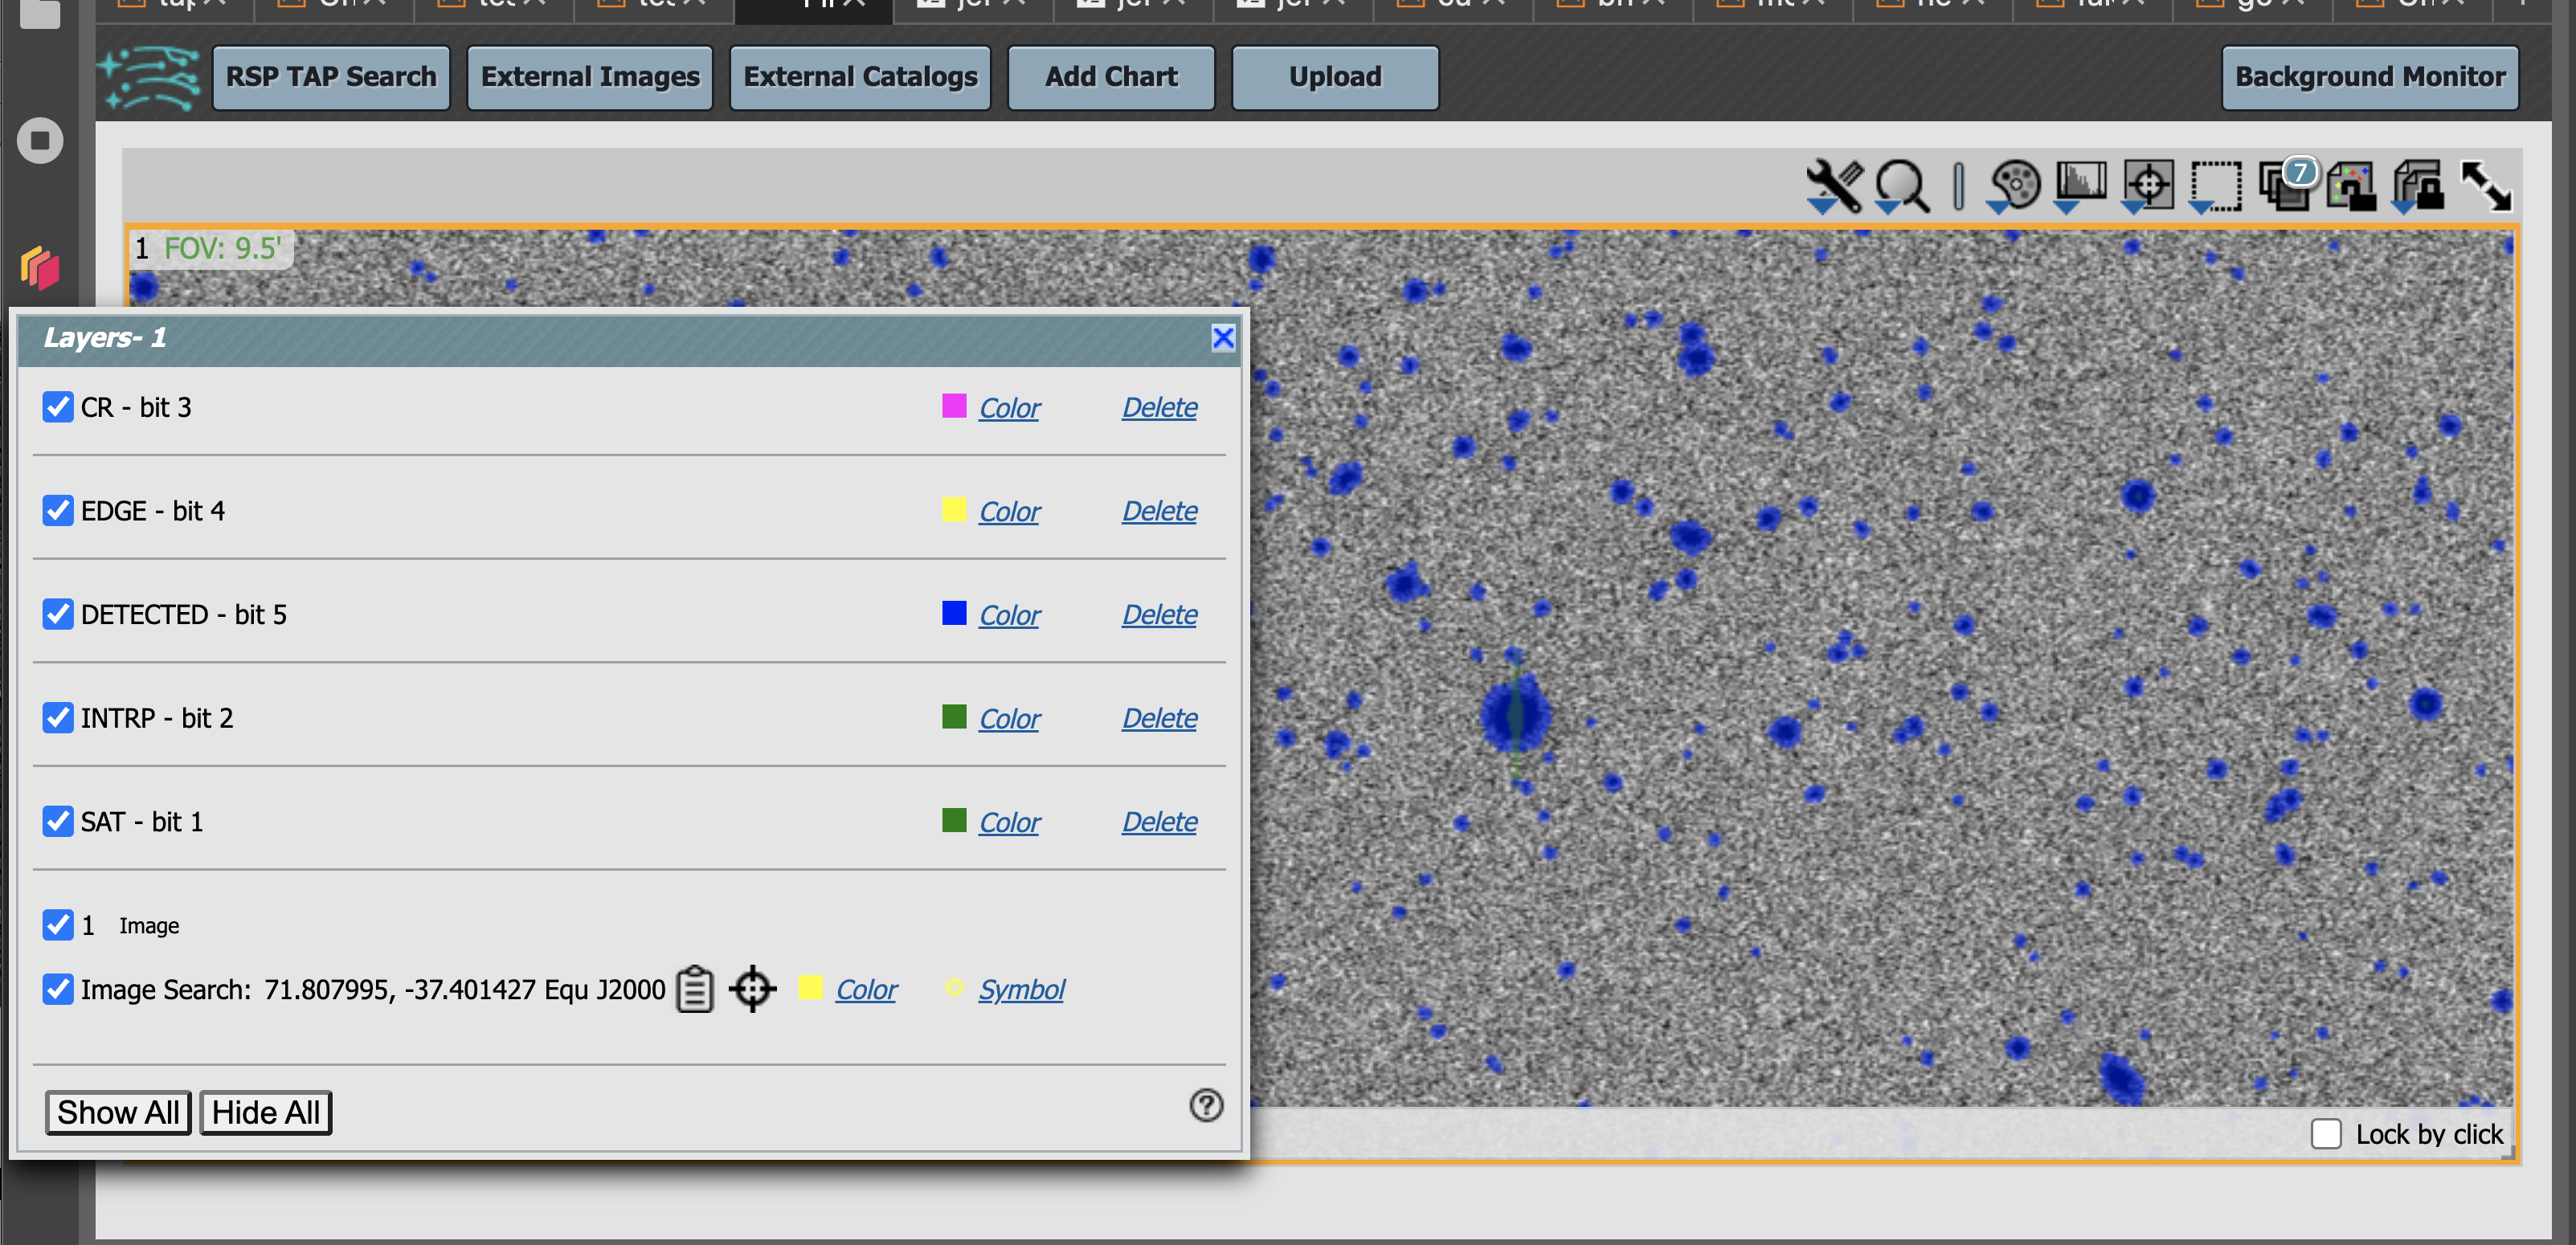
\includegraphics[width=4.25000in]{jira_imgs/3059.png}\\
The above image also shows the definitions of the different-colored mask
bits that are set.

}
\begin{tabular}{p{2cm}p{14cm}}
\toprule
Step 5 & Step Execution Status: \textbf{ Pass } \\ \hline
\end{tabular}
 Description \\
{\footnotesize
Plot images of the PSF model at various points, and verify that the PSF
differs with position.

}
\hdashrule[0.5ex]{\textwidth}{1pt}{3mm}
  Expected Result \\
{\footnotesize
A ``star-like'' image of the PSF evaluated at various positions. The PSF
should vary slightly with position (this could be readily visualized by
taking a difference of PSFs at two positions).

}
\hdashrule[0.5ex]{\textwidth}{1pt}{3mm}
  Actual Result \\
{\footnotesize
The following image shows the PSF extracted at two different positions
in the first two panels, and their difference in the third. The PSF is
clearly varying with position:\\
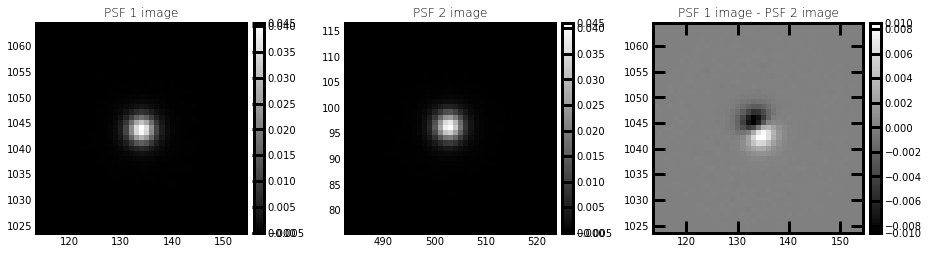
\includegraphics[width=5.78125in]{jira_imgs/3060.png}

}
\begin{tabular}{p{2cm}p{14cm}}
\toprule
Step 6 & Step Execution Status: \textbf{ Pass } \\ \hline
\end{tabular}
 Description \\
{\footnotesize
Starting from the XY pixel coordinates of the sources, apply the WCS to
obtain RA, Dec coordinates. Plot these positions and confirm that they
match the expected values from the WCS object.

}
\hdashrule[0.5ex]{\textwidth}{1pt}{3mm}
  Expected Result \\
{\footnotesize
RA, Dec coordinates that are returned should be near the central
position of the visit coordinate as given in either the calexp metadata
or the WCS.

}
\hdashrule[0.5ex]{\textwidth}{1pt}{3mm}
  Actual Result \\
{\footnotesize
We selected a single source from the catalog at
positions:\\[2\baselineskip]

\begin{verbatim}
(X, Y): ( 1730.342687466467 ,  386.1185560155262 )
(ra, dec): ( 71.89388932338906 ,  -37.34102758827357 )
\end{verbatim}

In the attached notebook, we confirmed that transforming between pixel
and sky coordinates gives the same result as the catalog. Here is the
output of the relevant cell:\\

\begin{verbatim}
RA, Dec from X, Y:  (71.8938893234, -37.3410275883)
X, Y from RA, Dec:  (1730.3, 386.12)
Sky to pixel agrees!
\end{verbatim}

}
\begin{tabular}{p{2cm}p{14cm}}
\toprule
Step 7 & Step Execution Status: \textbf{ Pass } \\ \hline
\end{tabular}
 Description \\
{\footnotesize
Repeat steps 2-6, but now with difference images created by the Alert
Production pipeline (for example, in the `ap\_verify` test data
processing).

}
\hdashrule[0.5ex]{\textwidth}{1pt}{3mm}
  Expected Result \\
{\footnotesize

}
\hdashrule[0.5ex]{\textwidth}{1pt}{3mm}
  Actual Result \\
{\footnotesize
See the results in the attached notebook, where we successfully verified
all of the PVI content for a difference image and its associated diaSrc
catalog.

}

\paragraph{ LVV-T141 - Verify implementation of Production Monitoring }\mbox{}\\

Version \textbf{1}.
Status \textbf{Approved}.
Open  \href{https://jira.lsstcorp.org/secure/Tests.jspa#/testCase/LVV-T141}{\textit{ LVV-T141 } }
test case in Jira.

Demonstrate monitoring capabilities that give real-time view of pipeline
execution and production systems usage/load.

\textbf{ Preconditions}:\\
Data set and mechanism for Production Orchestration as outlined in
\href{https://jira.lsstcorp.org/secure/Tests.jspa\#/testCase/LVV-T140}{LVV-T140}.

Execution status: {\bf Pass }

Final comment:\\


Detailed steps results:

\begin{tabular}{p{2cm}p{14cm}}
\toprule
Step 1 & Step Execution Status: \textbf{ Pass } \\ \hline
\end{tabular}
 Description \\
{\footnotesize
Process data with the Data Release Production payload, starting from raw
science images and generating science data products, placing them in the
Data Backbone.

}
\hdashrule[0.5ex]{\textwidth}{1pt}{3mm}
  Expected Result \\
{\footnotesize

}
\hdashrule[0.5ex]{\textwidth}{1pt}{3mm}
  Actual Result \\
{\footnotesize
300 sq. degrees of simulated LSST data (DESC DC2) ~was processed as part
of the DP0.2 processing campaign at the Interim Data Facility. The
production orchestration software used was PanDA.~

}
\begin{tabular}{p{2cm}p{14cm}}
\toprule
Step 2 & Step Execution Status: \textbf{ Pass } \\ \hline
\end{tabular}
 Description \\
{\footnotesize
While DRP processing is executing, monitor the progress and resource
usage of processing.

}
\hdashrule[0.5ex]{\textwidth}{1pt}{3mm}
  Expected Result \\
{\footnotesize
Ability to monitor in real-time the orchestrated production processing,
including resource usage.

}
\hdashrule[0.5ex]{\textwidth}{1pt}{3mm}
  Actual Result \\
{\footnotesize
During the execution of jobs in the PanDA system, production, resources
usage was monitored via the PanDA monitoring interface.
~DOMA\_GOOGLE\_LSST\_Queues.png shows LSST processing jobs in in the
DOMA\_GOOGLE\_LSST\_* queues. DP02 Processing Runs.png shows a snapshot
of jobs jobs in the PanDA workflow monitor during processing.~

}

\paragraph{ LVV-T140 - Verify implementation of Production Orchestration }\mbox{}\\

Version \textbf{1}.
Status \textbf{Approved}.
Open  \href{https://jira.lsstcorp.org/secure/Tests.jspa#/testCase/LVV-T140}{\textit{ LVV-T140 } }
test case in Jira.

Demonstrate use of orchestration software to perform batch production on
LSST compute platform(s).

\textbf{ Preconditions}:\\


Execution status: {\bf Pass }

Final comment:\\


Detailed steps results:

\begin{tabular}{p{2cm}p{14cm}}
\toprule
Step 1 & Step Execution Status: \textbf{ Pass } \\ \hline
\end{tabular}
 Description \\
{\footnotesize
Identify an appropriate precursor dataset.

}
\hdashrule[0.5ex]{\textwidth}{1pt}{3mm}
  Expected Result \\
{\footnotesize

}
\hdashrule[0.5ex]{\textwidth}{1pt}{3mm}
  Actual Result \\
{\footnotesize
The dataset to be used is the DP0.2 / DESC DC2 dataset at the IDF. DP0.2
Production Processing used stack v23 on IDF's PanDA
system.\\[2\baselineskip]

}
\begin{tabular}{p{2cm}p{14cm}}
\toprule
Step 2 & Step Execution Status: \textbf{ Pass } \\ \hline
\end{tabular}
 Description \\
{\footnotesize
Execute a batch processing job using the orchestration system, and
confirm (manually and/or via QA tools typically used for HSC
reprocessing) that the pipeline executed and produced all expected
products (or error logs in cases of failure).

}
\hdashrule[0.5ex]{\textwidth}{1pt}{3mm}
  Expected Result \\
{\footnotesize
Calexp single-visit and coadd images, and associated catalogs, are
present in a Butler repository. Logs of the processing are available to
be inspected for identification of problems in the processing.

}
\hdashrule[0.5ex]{\textwidth}{1pt}{3mm}
  Actual Result \\
{\footnotesize
Batch processing was carried in the Google Cloud environment at the IDF.
The production orchestration system deployed and used at the IDF
(Interim Data Facility) was PanDA. The BPS (Batch Processing Service)
software (part of the LSST distribution) was used to interface between
the Butler and PanDA using a set of yaml job submission files. A set of
six PanDA job queues were established with different retry
characteristics and memory limits. In excess of 4,000 cores were
available in a number of queues and memory/core configurations within
the IDF. 20K raw exposures/visits were pre-loaded into S3 storage to be
processed via thePanDA system. After processing was complete, a copy of
the Butler registry was made for end user access. All batch processing
for DP0.2 is described in Jira ticket:
\href{https://jira.lsstcorp.org/browse/PREOPS-905}{PREOPS-905}. Report
https://rtn-039.lsst.io/ describes the full details of the DP0.2
production processing.\\[2\baselineskip]\# Logs of the processing\\
Google Cloud logging system was used to collect logging information
output by the production pipelines and organize it into a searchable
form sorted by date of production. Snapshots of logs showing the status
of jobs is attached.\\[2\baselineskip]\# Show that single visit, coadds
and catalogs are present in the DP0.2 Butler repository.\\
These data products can be accessed via the DP0.2 Butler
programmatically at the IDF with the attached script. This clearly shows
the availability of processed data products

}

\paragraph{ LVV-T129 - Verify implementation of Provide Calibrated Photometry }\mbox{}\\

Version \textbf{1}.
Status \textbf{Approved}.
Open  \href{https://jira.lsstcorp.org/secure/Tests.jspa#/testCase/LVV-T129}{\textit{ LVV-T129 } }
test case in Jira.

Verify that the DMS provides photometry calibrated in AB mags and fluxes
(in nJy) for all measured objects and sources. Must be tested for both
DRP and AP products.

\textbf{ Preconditions}:\\


Execution status: {\bf Initial Pass }

Final comment:\\Executed at the IDF using Science Pipelines version w\_2022\_32. A
portion of this test case can be executed by running the script
test\_LVV-T129.py, which is available in the test report github
repository's ``scripts/'' directory. Qserv tables (i.e., Object tables)
were checked via the notebook test\_LVV-T129.ipynb, which is available
in the test report github repository's ``notebooks''
directory.\\[2\baselineskip]This Test Case is granted status of
``Initial Pass'' because the DIAObject table in Qserv does not clearly
demonstrate that fluxes are provided in nJy. Though the fluxes are shown
to be reasonable values if they are in nJy (and inspection of code could
confirm this), we choose not to grant this test a full PASS until the
DIAObject table is clearly reporting fluxes in nJy.


Detailed steps results:

\begin{tabular}{p{2cm}p{14cm}}
\toprule
Step 1 & Step Execution Status: \textbf{ Pass } \\ \hline
\end{tabular}
 Description \\
{\footnotesize
Identify the path to the data repository, which we will refer to as
`DATA/path', then execute the following:

}
\hdashrule[0.5ex]{\textwidth}{1pt}{3mm}
  Example Code \\
{\footnotesize
\begin{verbatim}
from lsst.daf.butler import Butler
repo = 'Data/path'
collection = 'collection'
butler = Butler(repo, collections=collection)
\end{verbatim}

}
\hdashrule[0.5ex]{\textwidth}{1pt}{3mm}
  Expected Result \\
{\footnotesize
Butler repo available for reading.

}
\hdashrule[0.5ex]{\textwidth}{1pt}{3mm}
  Actual Result \\
{\footnotesize
Tests were performed by executing test\_LVV-T28.py, which contains the
following:\\[2\baselineskip]\# For DP0.2 data on the IDF:\\
config = `dp02'\\
collection = `2.2i/runs/DP0.2'\\
butler = Butler(config, collections=collection)

}
\begin{tabular}{p{2cm}p{14cm}}
\toprule
Step 2 & Step Execution Status: \textbf{ Pass } \\ \hline
\end{tabular}
 Description \\
{\footnotesize
Ingest the data products from an appropriate DRP-processed dataset.

}
\hdashrule[0.5ex]{\textwidth}{1pt}{3mm}
  Expected Result \\
{\footnotesize

}
\hdashrule[0.5ex]{\textwidth}{1pt}{3mm}
  Actual Result \\
{\footnotesize
By default, the test script contains the following detector/visit
combination. This can be changed if desired.\\[2\baselineskip]\# Select
an arbitrary source catalog from a PVI and difference image:\\
instrument = `LSSTCam-imSim'\\
detector = 5\\
visit = 924041\\[2\baselineskip]\# Run the test\\
python test\_LVV-T129

}
\begin{tabular}{p{2cm}p{14cm}}
\toprule
Step 3 & Step Execution Status: \textbf{ Pass } \\ \hline
\end{tabular}
 Description \\
{\footnotesize
Confirm that AB-calibrated magnitudes and fluxes are available for all
measured Sources and Objects. {[}An enhanced verification could include
matching the sources to an external source catalog and comparing the
magnitudes to show that they are well-calibrated.{]}

}
\hdashrule[0.5ex]{\textwidth}{1pt}{3mm}
  Expected Result \\
{\footnotesize
Calibrated fluxes and magnitudes are available for all sources, as well
as tools to convert measured fluxes to magnitudes (and vice-versa).

}
\hdashrule[0.5ex]{\textwidth}{1pt}{3mm}
  Actual Result \\
{\footnotesize
The test script confirms that AB-calibrated magnitudes and fluxes in nJy
are available for all Sources. This is checked for both PVIs (i.e.,
``calexps'') and difference images.The script also compares the results
from the Science Pipelines to those calculated via transformations from
nJy to ABmag in `astropy` tools.\\[2\baselineskip]python
test\_LVV-T129.py\\
lsst\_distrib g0b29ad24fb+cafeaf151e current w\_2022\_32 setup\\
Input dataId: \{'instrument': `LSSTCam-imSim', `visit': 924041,
`detector': 5\}\\[2\baselineskip]TRUE: src table fluxes are available in
calibrated nJy and ABmag.\\
Input dataId: \{'instrument': `LSSTCam-imSim', `visit': 924041,
`detector': 5\}\\[2\baselineskip]TRUE: goodSeeingDiff\_diaSrc table
fluxes are available in calibrated nJy and ABmag.

}
\begin{tabular}{p{2cm}p{14cm}}
\toprule
Step 4 & Step Execution Status: \textbf{ Pass } \\ \hline
\end{tabular}
 Description \\
{\footnotesize
Ingest the data products from an appropriate AP processing dataset.

}
\hdashrule[0.5ex]{\textwidth}{1pt}{3mm}
  Expected Result \\
{\footnotesize

}
\hdashrule[0.5ex]{\textwidth}{1pt}{3mm}
  Actual Result \\
{\footnotesize
This was confirmed in Step 3 for single-visit AP processing. In the
following step, we will confirm the fluxes and magnitudes for Object
tables.

}
\begin{tabular}{p{2cm}p{14cm}}
\toprule
Step 5 & Step Execution Status: \textbf{ Initial Pass } \\ \hline
\end{tabular}
 Description \\
{\footnotesize
Confirm that AB-calibrated magnitudes and fluxes are available for all
measured Sources, DIASources, and Objects. {[}An enhanced verification
could include matching the sources to an external source catalog and
comparing the magnitudes to show that they are well-calibrated.{]}

}
\hdashrule[0.5ex]{\textwidth}{1pt}{3mm}
  Expected Result \\
{\footnotesize
Calibrated fluxes and magnitudes are available for all Sources,
DIASources, and Objects, as well as tools to convert measured fluxes to
magnitudes (and vice-versa).

}
\hdashrule[0.5ex]{\textwidth}{1pt}{3mm}
  Actual Result \\
{\footnotesize
For the Object and DIAObject tables, we instead query the Qserv database
via the Rubin Science Platform. The results are seen in notebook
test\_LVV-T129.ipynb.\\[2\baselineskip]The notebook demonstrates that
the Object table (i.e., measurements from DRP processed coadd images)
meets the requirement -- all fluxes are in calibrated nanoJanskys.
However, the DIAObject table does not report units with the flux values.
Although we show in the attached notebook that these fluxes have
reasonable values assuming they are in nJy, the lack of units in the
database and schema leads us to characterize this step of the test as an
INITIAL PASS. An issue has been created to fix this, and the test case
will be executed again in the futue.

}

\paragraph{ LVV-T127 - Verify implementation of Provide Source Detection Software }\mbox{}\\

Version \textbf{1}.
Status \textbf{Approved}.
Open  \href{https://jira.lsstcorp.org/secure/Tests.jspa#/testCase/LVV-T127}{\textit{ LVV-T127 } }
test case in Jira.

Verify that the DMS provides source detection software that can be
applied to calibrated images, including both difference images and
coadds. This will be verified using simulated data, but could also be
done by inserting artificial sources into existing datasets.

\textbf{ Preconditions}:\\


Execution status: {\bf Pass }

Final comment:\\See attached artifact notebook ``test\_LVV-T127.ipynb'' for details.


Detailed steps results:

\begin{tabular}{p{2cm}p{14cm}}
\toprule
Step 1 & Step Execution Status: \textbf{ Pass } \\ \hline
\end{tabular}
 Description \\
{\footnotesize
Run DRP and AP processing, including source detection and measurement
algorithms, on a small portion of the data from a simulated dataset.

}
\hdashrule[0.5ex]{\textwidth}{1pt}{3mm}
  Expected Result \\
{\footnotesize
Source catalogs containing measurements of all sources detected in the
input images.

}
\hdashrule[0.5ex]{\textwidth}{1pt}{3mm}
  Actual Result \\
{\footnotesize
For this test, we use Data Preview 0.2 data, which is the reprocessed
version of the simulated DC2 dataset. All work for this test took place
in the notebook ``test\_LVV-T127.ipynb'', which is archived alongside
the Test Report for this campaign.\\[2\baselineskip]In the notebook, a
number of explorations show that the source detection and measurement
algorithms ran, and produced reasonable measurements, as required.

}
\begin{tabular}{p{2cm}p{14cm}}
\toprule
Step 2 & Step Execution Status: \textbf{ Pass } \\ \hline
\end{tabular}
 Description \\
{\footnotesize
Confirm that the output repos contain catalogs of source detections.
Compare these output catalogs to the original simulated source catalogs,
and confirm that a large fraction of the sources within a reasonable
signal-to-noise range were recovered.

}
\hdashrule[0.5ex]{\textwidth}{1pt}{3mm}
  Expected Result \\
{\footnotesize
Most sources above a reasonable S/N threshold were detected, and their
measured fluxes are reasonably close to the simulated inputs.

}
\hdashrule[0.5ex]{\textwidth}{1pt}{3mm}
  Actual Result \\
{\footnotesize
We demonstrate in the notebook (from which the figure below is derived)
that sources are detected to a limit of S/N\textgreater{}5, which
reaches a depth of at least 24th
magnitude.\\[2\baselineskip]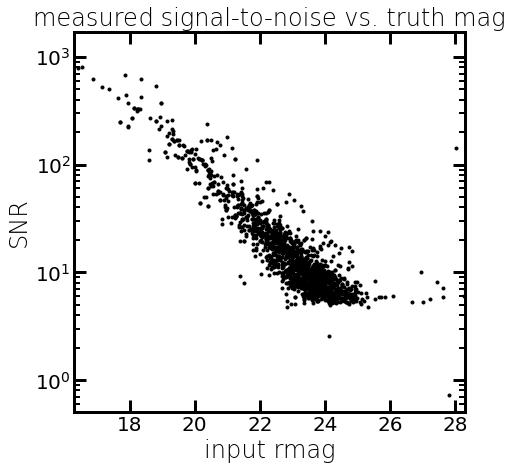
\includegraphics[width=3.12500in]{jira_imgs/3038.png}\\
We also demonstrate that the measurements agree with the ``true'' fluxes
of the simulated sources rather well:\\
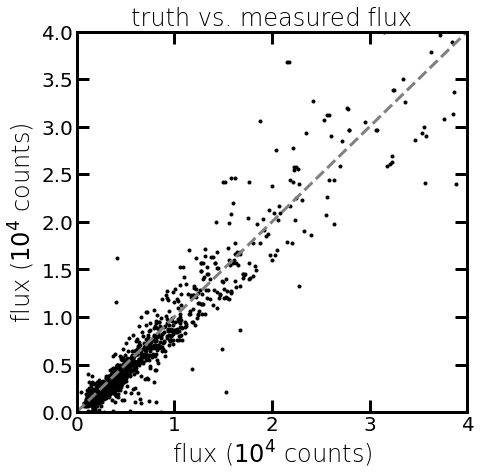
\includegraphics[width=3.12500in]{jira_imgs/3039.png}

}

\paragraph{ LVV-T79 - Verify implementation of PSF-Matched Coadds }\mbox{}\\

Version \textbf{1}.
Status \textbf{Approved}.
Open  \href{https://jira.lsstcorp.org/secure/Tests.jspa#/testCase/LVV-T79}{\textit{ LVV-T79 } }
test case in Jira.

Verify that the DRP pipelines produce PSF matched coadds.

\textbf{ Preconditions}:\\


Execution status: {\bf Pass }

Final comment:\\


Detailed steps results:

\begin{tabular}{p{2cm}p{14cm}}
\toprule
Step 1 & Step Execution Status: \textbf{ Pass } \\ \hline
\end{tabular}
 Description \\
{\footnotesize
Execute the AssembleCoaddTask, specifying via configuration that
PSF-matched coadds should be created.

}
\hdashrule[0.5ex]{\textwidth}{1pt}{3mm}
  Expected Result \\
{\footnotesize
Pipetask executes and produces coadd images.

}
\hdashrule[0.5ex]{\textwidth}{1pt}{3mm}
  Actual Result \\
{\footnotesize
Working on the USDF (SLAC) with the LSST Science Pipelines set up, we
defined a brief pipeline that explicitly specifies that `psfMatched`
warps should be created. For this test, we use the `rc2\_subset` data,
which has already been processed from end to end. The PSF-matched warps
are created in the `step3` subset of `rc2\_subset` processing, so we can
use those to create a PSF-matched coadd.\\[2\baselineskip]Contents of
psfmatched\_coadd.yaml:\\[2\baselineskip]description: The DRP pipeline
specialized for rc2\_subset processing in jenkins and tutorials\\
imports:\\
- \$DRP\_PIPE\_DIR/pipelines/HSC/DRP-RC2.yaml\\
tasks:\\
assemblePsfMatchedCoadd:\\
class: lsst.pipe.tasks.assembleCoadd.AssembleCoaddTask\\
config:\\
warpType: psfMatched\\[2\baselineskip]Execute the pipeline as follows:\\
pipetask run -b \$RC2\_SUBSET\_DIR/SMALL\_HSC/butler.yaml -d ``tract =
9813 AND skymap = `hsc\_rings\_v1' AND patch in (38, 39, 40, 41) AND
band='i''' -p
\$RC2\_\_DIR/psfmatched\_coadd.yaml\#assemblePsfMatchedCoadd -i
u/\$USER/step3 -o u/\$USER/psf\_matched\_coadds --register-dataset-types
-j 4\\[2\baselineskip]This pipeline executed its 4 quanta in about 5
minutes.

}
\begin{tabular}{p{2cm}p{14cm}}
\toprule
Step 2 & Step Execution Status: \textbf{ Pass } \\ \hline
\end{tabular}
 Description \\
{\footnotesize
Identify the path to the data repository, which we will refer to as
`DATA/path', then execute the following:

}
\hdashrule[0.5ex]{\textwidth}{1pt}{3mm}
  Example Code \\
{\footnotesize
\begin{verbatim}
from lsst.daf.butler import Butler
repo = 'Data/path'
collection = 'collection'
butler = Butler(repo, collections=collection)
\end{verbatim}

}
\hdashrule[0.5ex]{\textwidth}{1pt}{3mm}
  Expected Result \\
{\footnotesize
Butler repo available for reading.

}
\hdashrule[0.5ex]{\textwidth}{1pt}{3mm}
  Actual Result \\
{\footnotesize
from lsst.daf.butler import Butler\\
repo =
`/sdf/data/rubin/u/jcarlin/repos/rc2\_subset/SMALL\_HSC'\\[2\baselineskip]\#
Output collection from pipetask run in Step 1:\\
collection = `u/jcarlin/psf\_matched\_coadds'\\
butler = Butler(repo, collections=collection)\\[2\baselineskip]\#
Initialize a second Butler pointing to the original rc2\_subset
processing:\\
collection2 = `u/jcarlin/step3'\\
butler2 = Butler(repo, collections=collection2)\\[2\baselineskip]

}
\begin{tabular}{p{2cm}p{14cm}}
\toprule
Step 3 & Step Execution Status: \textbf{ Pass } \\ \hline
\end{tabular}
 Description \\
{\footnotesize
Verify that PSF-matched coadds were created.

}
\hdashrule[0.5ex]{\textwidth}{1pt}{3mm}
  Expected Result \\
{\footnotesize

}
\hdashrule[0.5ex]{\textwidth}{1pt}{3mm}
  Actual Result \\
{\footnotesize
In an ipython session, we executed the following commands. The object is
to demonstrate (a) that the coadd was created, and (b) that the
PSF-matched coadd differs from the direct coadd in the ``step3''
collection.\\[2\baselineskip]\# Is ``coadd'' an Exposure object?\\
coadd\\
Out{[}29{]}: \textless{}lsst.afw.image.exposure.ExposureF at
0x7f9be81e4db0\textgreater{}\\[2\baselineskip]Yes, it is a non-empty
exposure. Next, extract the newly-created, PSF-matched coadd and the
direct-warp coadd, and compare their pixel
values.\\[2\baselineskip]import numpy as np\\[2\baselineskip]\# Get the
PSF-matched coadd:\\
coadd = butler.get('deepCoadd', tract=9813, patch=38,
band='i')\\[2\baselineskip]\# Get the direct coadd:\\
coadd2 = butler2.get('deepCoadd', tract=9813, patch=38,
band='i')\\[2\baselineskip]\# Copy the PSF-matched coadd:\\
coadd\_copy = coadd.clone()\\
\# Subtract the direct coadd's image array from the PSF-matched image
array:\\
coadd\_copy.image.array -= coadd2.image.array\\[2\baselineskip]\#
Extract some statistics of the resulting array:\\
In {[}26{]}: np.mean(coadd\_copy.image.array)\\
Out{[}26{]}:~1.31110555e-05\\[2\baselineskip]In
{[}27{]}:~np.median(coadd\_copy.image.array)\\
Out{[}27{]}:~1.4901161e-08\\[2\baselineskip]In
{[}28{]}:~np.std(coadd\_copy.image.array)\\
Out{[}28{]}: 0.0049309013\\[2\baselineskip]The two coadd images differ,
but only by a small amount, which is verification that the PSF-matched
coadd has been created successfully.

}

\paragraph{ LVV-T1830 - Verify Implementation of Scientific Visualization of Camera Image Data }\mbox{}\\

Version \textbf{1}.
Status \textbf{Approved}.
Open  \href{https://jira.lsstcorp.org/secure/Tests.jspa#/testCase/LVV-T1830}{\textit{ LVV-T1830 } }
test case in Jira.

Verify that all scientific visualization of camera image data uses the
coordinate systems defined in \href{https://lse-349.lsst.io/}{LSE-349}.

\textbf{ Preconditions}:\\


Execution status: {\bf Pass }

Final comment:\\


Detailed steps results:

\begin{tabular}{p{2cm}p{14cm}}
\toprule
Step 1 & Step Execution Status: \textbf{ Pass } \\ \hline
\end{tabular}
 Description \\
{\footnotesize
Identify an image containing bright saturated stars. Load this image
into an image viewer such as Firefly or DS9.

}
\hdashrule[0.5ex]{\textwidth}{1pt}{3mm}
  Expected Result \\
{\footnotesize
Image with bright stars is displayed.

}
\hdashrule[0.5ex]{\textwidth}{1pt}{3mm}
  Actual Result \\
{\footnotesize
Via the RSP Portal aspect, we executed a search of the Source table over
a 5-degree radius, with constraints ``pixelFlags\_saturated = 1,''
~``pixelFlags\_saturatedCenter = 1,'' and ``detect\_isPrimary = 1'' to
identify saturated stars. We then took the necessary information to
create a dataId, and selected the corresponding calexp image within the
Notebook aspect. The dataId and relevant commands from the notebook
are:\\[2\baselineskip]from lsst.daf.butler import Butler\\
import lsst.afw.display as afwDisplay\\
from firefly\_client import FireflyClient\\[2\baselineskip]config =
`dp02'\\
collection = `2.2i/runs/DP0.2'\\
butler = Butler(config, collections=collection)\\[2\baselineskip]dataId
= \{'instrument': `LSSTCam-imSim', `detector': 180, `visit': 888370,
`exposure':888370, `band':'g'\}\\
calexp = butler.get('calexp',
dataId=dataId)\\[2\baselineskip]afwDisplay.setDefaultBackend('firefly')\\
afw\_display = afwDisplay.Display(frame=1)\\
afw\_display.mtv(calexp)\\[2\baselineskip]This results in a calexp image
displayed in Firefly.

}
\begin{tabular}{p{2cm}p{14cm}}
\toprule
Step 2 & Step Execution Status: \textbf{ Pass } \\ \hline
\end{tabular}
 Description \\
{\footnotesize
Confirm that each of the following is true:\\

\begin{itemize}
\tightlist
\item
  the XY coordinate origin is at the lower left,
\item
  the x-coordinate increases left-to-right, and the y-coordinate
  increases bottom-to-top
\item
  bleed trails of saturated stars are vertical (i.e., the parallel
  transfer direction is oriented vertically)
\item
  the sky orientation places east 90 degrees counter-clockwise from
  north
\end{itemize}

}
\hdashrule[0.5ex]{\textwidth}{1pt}{3mm}
  Expected Result \\
{\footnotesize
Via coordinate grid overlays or similar, an image is demonstrated to
meet the necessary conditions.

}
\hdashrule[0.5ex]{\textwidth}{1pt}{3mm}
  Actual Result \\
{\footnotesize
In the first screenshot, we use the ``extract line from image'' tool to
demonstrate the first two conditions. The red arrow selecting pixels for
statistics begins at the lower left corner, and the inset plot says
``Line Extract Preview - (0, 0) to (19, 0)'', thus confirming that the
lower-left corner is the coordinate origin. The arrow shows
directionality, so that the figure demonstrates the arrowhead is at
coordinate (19, 0). This confirms that the x-coordinate increases
left-to-right. We confirmed that the y-coordinate increases vertically
by a similar method.\\
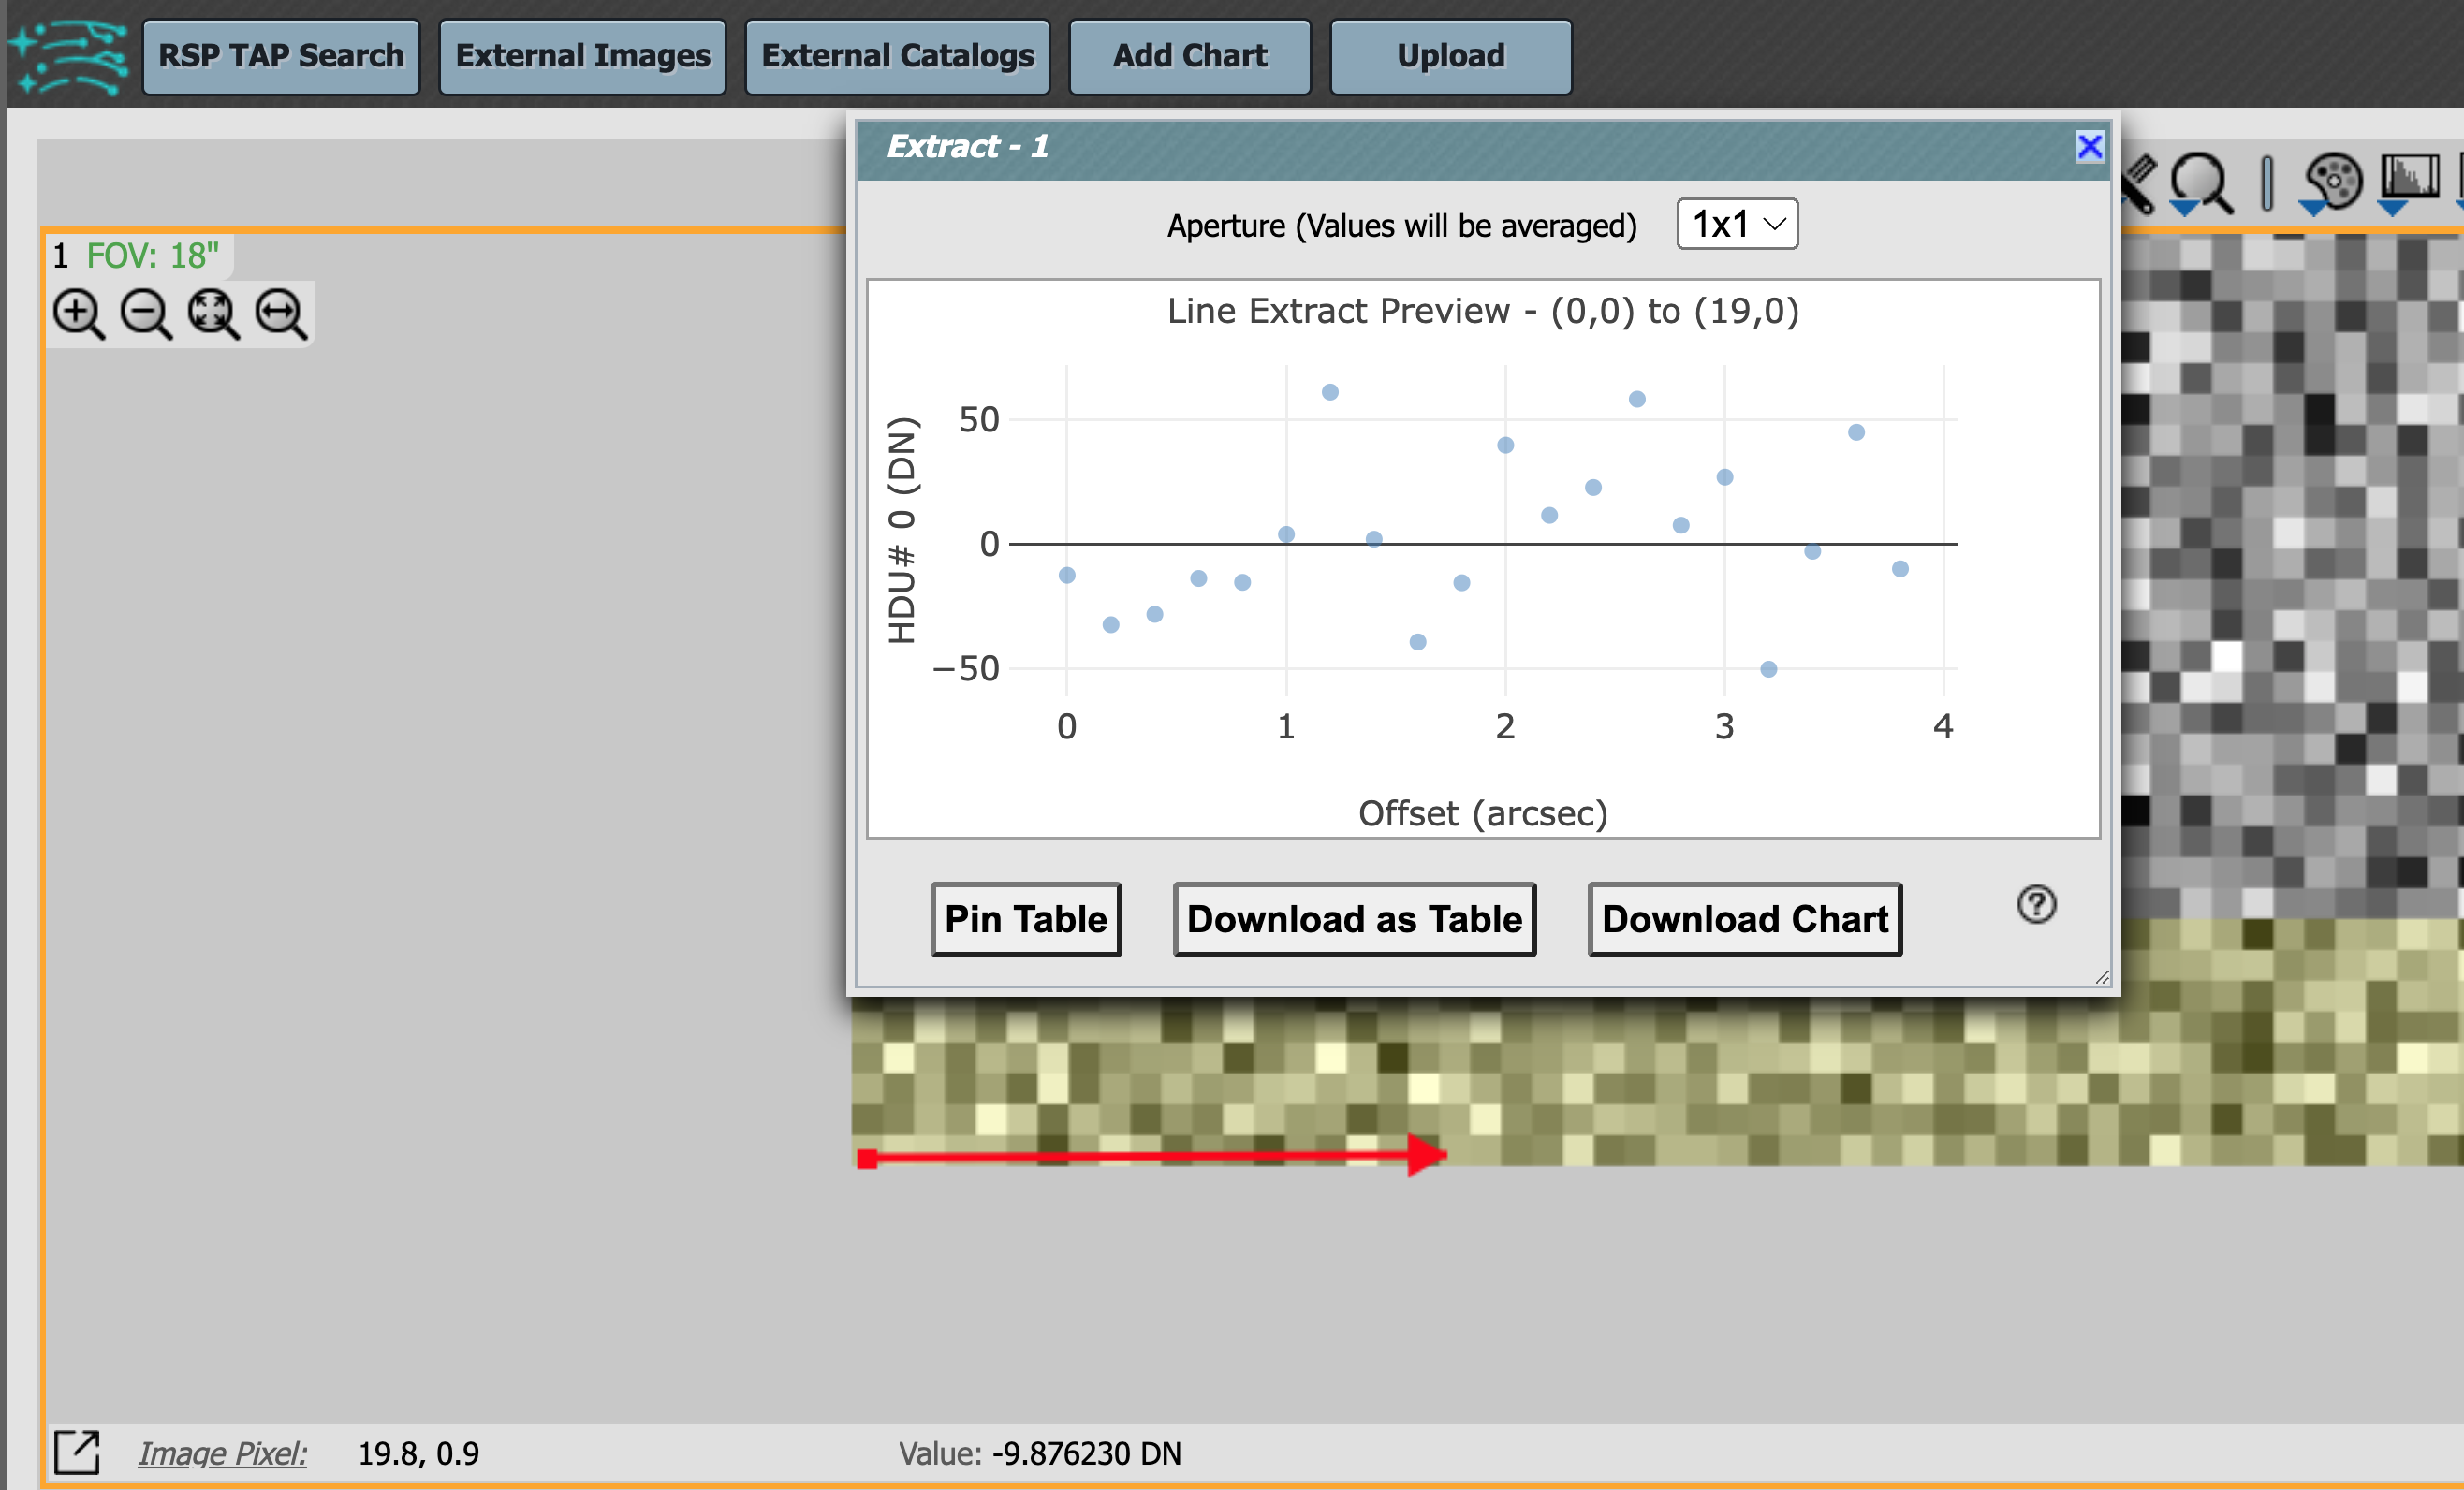
\includegraphics[width=5.14583in]{jira_imgs/3064.png}\\
The next screenshot shows two saturated stars. The mask plane has been
displayed atop the image, with pixels flagged as ``SATURATED'' shown in
green. From the two saturated stars, it is clear that bleed trails are
oriented vertically. Finally, the sky orientation is shown by the yellow
arrows near the upper left, which demonstrate that east is oriented 90
degrees counter-clockwise from north, as required.\\
\includegraphics[width=5.22917in]{jira_imgs/3065.png}\\
We have thus demonstrated that camera image data is visualized using the
coordinates as defined in LSE-349.

}

\paragraph{ LVV-T145 - Verify implementation of Task Configuration }\mbox{}\\

Version \textbf{1}.
Status \textbf{Approved}.
Open  \href{https://jira.lsstcorp.org/secure/Tests.jspa#/testCase/LVV-T145}{\textit{ LVV-T145 } }
test case in Jira.

Verify that the DMS software provides configuration control to define,
override, and verify the configuration for a DMS Task.

\textbf{ Preconditions}:\\


Execution status: {\bf Pass }

Final comment:\\


Detailed steps results:

\begin{tabular}{p{2cm}p{14cm}}
\toprule
Step 1 & Step Execution Status: \textbf{ Pass } \\ \hline
\end{tabular}
 Description \\
{\footnotesize
Inspect software design to verify that one can define the configuration
for a Task.

}
\hdashrule[0.5ex]{\textwidth}{1pt}{3mm}
  Expected Result \\
{\footnotesize

}
\hdashrule[0.5ex]{\textwidth}{1pt}{3mm}
  Actual Result \\
{\footnotesize
As an example, take
\href{https://github.com/lsst/ip_isr/blob/main/python/lsst/ip/isr/isrTask.py}{isrTask}.
Inspection reveals the following, which is a portion of the
configuration for
IsrTask:\\[2\baselineskip]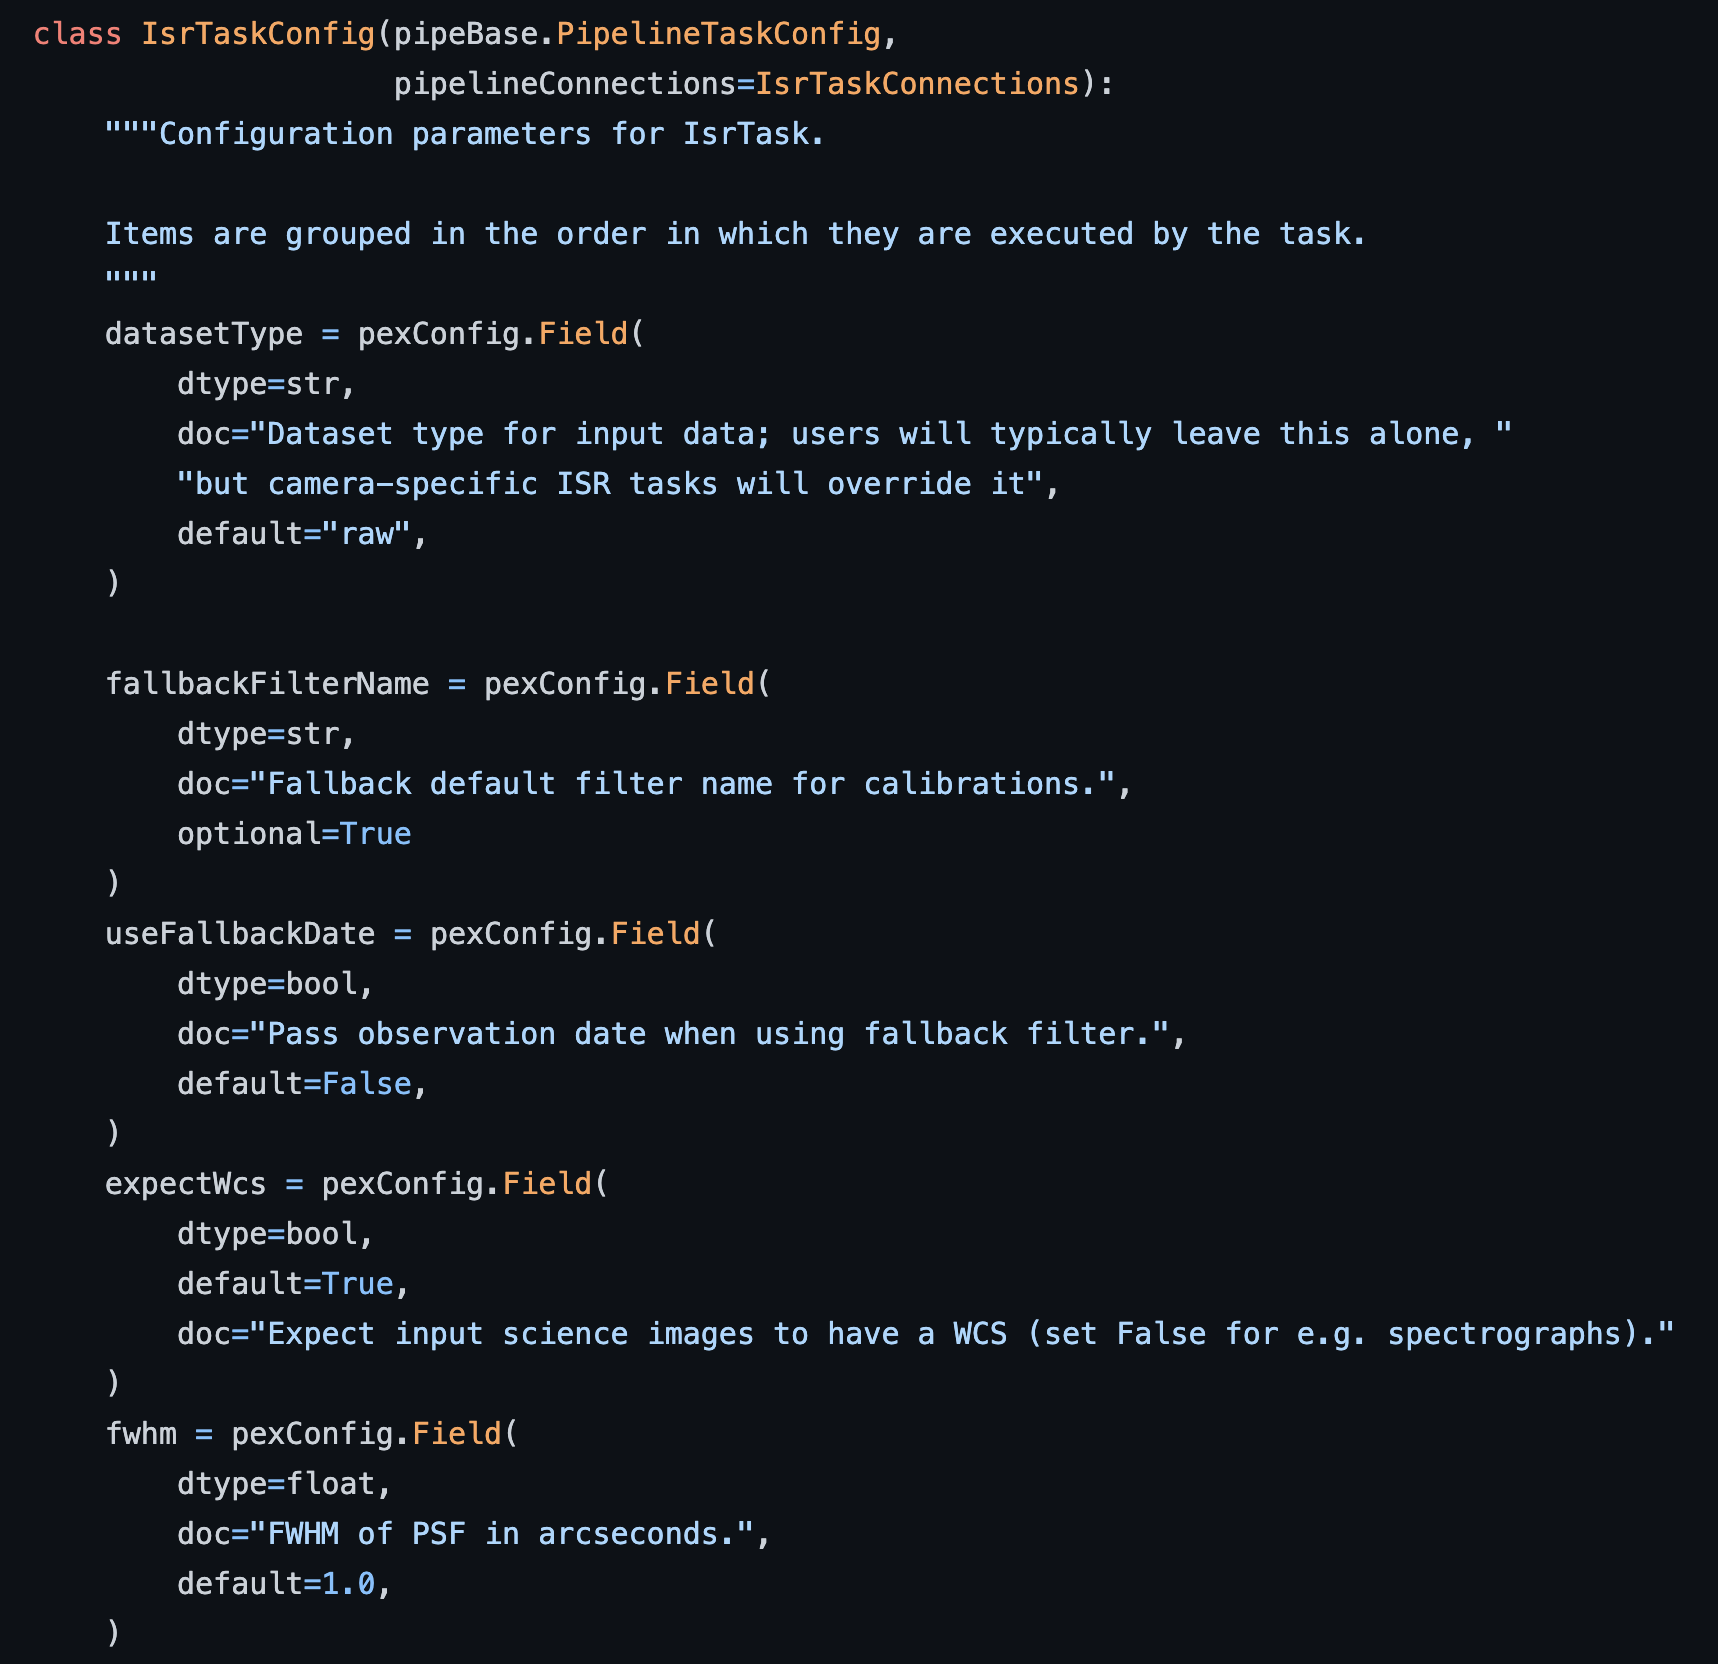
\includegraphics[width=4.22917in]{jira_imgs/3071.png}

}
\begin{tabular}{p{2cm}p{14cm}}
\toprule
Step 2 & Step Execution Status: \textbf{ Pass } \\ \hline
\end{tabular}
 Description \\
{\footnotesize
Run a Task with a known invalid configuration. ~Verify that the error is
caught before the science algorithm executes.

}
\hdashrule[0.5ex]{\textwidth}{1pt}{3mm}
  Expected Result \\
{\footnotesize

}
\hdashrule[0.5ex]{\textwidth}{1pt}{3mm}
  Actual Result \\
{\footnotesize
With the science pipelines w\_2022\_35 set up on the USDF devl machines,
execute the following:\\[2\baselineskip]setup -j -r
/sdf/group/rubin/u/jcarlin/repos/rc2\_subset/\\
export NUMPROC=8\\[2\baselineskip]Copy the default pipeline for the
rc2\_subset processing. We will modify this for each test step.\\
cp \$RC2\_SUBSET\_DIR/pipelines/DRP.yaml ./\\[2\baselineskip]Edit this
file to contain the (deliberately wrong) configuration:\\
tasks:\\
\hspace*{0.333em} characterizeImage:\\
\hspace*{0.333em} ~ class:
lsst.pipe.tasks.characterizeImage.CharacterizeImageTask\\
\hspace*{0.333em} ~ config:\\
\hspace*{0.333em} ~ ~ detection.thresholdValue:
`starwars'\\[2\baselineskip]Execute the pipeline task for
``step1'':\\[2\baselineskip]pipetask --long-log run -j \$NUMPROC -b
\$\{RC2\_SUBSET\_DIR\}/SMALL\_HSC/butler.yaml -p DRP.yaml\#nightlyStep1
-i HSC/RC2/defaults --register-dataset-types -o u/\$USER/LVV-T145\_step1
-d ``detector in (42) AND visit in (11690,
11698)''\\[2\baselineskip]pipetask --long-log run -j \$NUMPROC -b
\$\{RC2\_SUBSET\_DIR\}/SMALL\_HSC/butler.yaml -p DRP.yaml\#nightlyStep1
-i HSC/RC2/defaults --register-dataset-types -o
u/\$USER/LVV-T145\_step1\\[2\baselineskip]As expected, this fails with
the following error:\\[2\baselineskip]ERROR
2022-08-30T15:02:50.570-07:00 lsst.daf.butler.cli.utils
()(utils.py:1049) - Caught an exception, details are in traceback:\\
Traceback (most recent call last):\\
\hspace*{0.333em}\hspace*{0.333em}File
``/sdf/group/rubin/sw/conda/envs/lsst-scipipe-4.1.0/share/eups/Linux64/pex\_config/g849534e15f+3b870f08dc/python/lsst/pex/config/config.py'',
line 801, in \_\_set\_\_\\
\hspace*{0.333em} ~~self.\_validateValue(value)\\
\hspace*{0.333em}\hspace*{0.333em}File
``/sdf/group/rubin/sw/conda/envs/lsst-scipipe-4.1.0/share/eups/Linux64/pex\_config/g849534e15f+3b870f08dc/python/lsst/pex/config/rangeField.py'',
line 144, in \_validateValue\\
\hspace*{0.333em} ~~Field.\_validateValue(self, value)\\
\hspace*{0.333em}\hspace*{0.333em}File
``/sdf/group/rubin/sw/conda/envs/lsst-scipipe-4.1.0/share/eups/Linux64/pex\_config/g849534e15f+3b870f08dc/python/lsst/pex/config/config.py'',
line 628, in \_validateValue\\
\hspace*{0.333em} ~~raise TypeError(msg)\\
TypeError: Value starwars is of incorrect type str. Expected type
float\\[2\baselineskip]We have thus verified that an invalid
configuration causes an error before the tasks execute.

}
\begin{tabular}{p{2cm}p{14cm}}
\toprule
Step 3 & Step Execution Status: \textbf{ Pass } \\ \hline
\end{tabular}
 Description \\
{\footnotesize
Run a simple task with two different configurations that make a material
difference for a Task. ~E.g., specify a different source detection
threshold. ~Verify that the configuration is different between the two
runs through difference in recorded provenance and in results.

}
\hdashrule[0.5ex]{\textwidth}{1pt}{3mm}
  Expected Result \\
{\footnotesize

}
\hdashrule[0.5ex]{\textwidth}{1pt}{3mm}
  Actual Result \\
{\footnotesize
Now we will change the threshold from the previous step to a valid
numerical value. We will then run the task with two different values for
this detection threshold, and confirm that the results
differ.\\[2\baselineskip]tasks:\\
characterizeImage:\\
class: lsst.pipe.tasks.characterizeImage.CharacterizeImageTask\\
config:\\
detection.thresholdValue: 100\\[2\baselineskip]pipetask --long-log run
-j \$NUMPROC -b \$\{RC2\_SUBSET\_DIR\}/SMALL\_HSC/butler.yaml -p
DRP.yaml\#nightlyStep1 -i HSC/RC2/defaults --register-dataset-types -o
u/\$USER/LVV-T145\_step1\_thresh100 -d ``detector in (42) AND visit in
(11690, 11698)''\\[2\baselineskip]Now change the threshold to 30, and
run the pipetask again, specifying u/\$USER/LVV-T145\_step1\_thresh30 as
the output collection.\\[2\baselineskip]The attached script
``test\_LVV-T145.py'' reads the `src` catalog from each of the two
collections in turn, and compares the number of sources in each
catalog.\\[2\baselineskip]Executing this prints the following to the
screen:\\
python test\_LVV-T145.py\\[2\baselineskip]lsst\_distrib
g0b29ad24fb+434521fcbd current w\_2022\_35 setup\\
src1 length:~~3172\\
src2 length:~~3212\\
run1 threshold:~~100.0\\
run2 threshold:~~30.0\\[2\baselineskip]This confirms that the change in
threshold affected the number of detected sources, and that the
thresholds were persisted in metadata in the butler collections.

}

\paragraph{ LVV-T144 - Verify implementation of Task Specification }\mbox{}\\

Version \textbf{1}.
Status \textbf{Approved}.
Open  \href{https://jira.lsstcorp.org/secure/Tests.jspa#/testCase/LVV-T144}{\textit{ LVV-T144 } }
test case in Jira.

Verify that the DMS provides the ability to define a new or modified
pipeline task without recompilation.

\textbf{ Preconditions}:\\


Execution status: {\bf Pass }

Final comment:\\


Detailed steps results:

\begin{tabular}{p{2cm}p{14cm}}
\toprule
Step 1 & Step Execution Status: \textbf{ Pass } \\ \hline
\end{tabular}
 Description \\
{\footnotesize
Inspect software architecture. ~Verify that there exist Tasks that can
be run and configured without re-compilation.

}
\hdashrule[0.5ex]{\textwidth}{1pt}{3mm}
  Expected Result \\
{\footnotesize
Confirmation that the software architecture has allowed for
reconfiguring and running Tasks without recompilation.

}
\hdashrule[0.5ex]{\textwidth}{1pt}{3mm}
  Actual Result \\
{\footnotesize
As an example, take
\href{https://github.com/lsst/ip_isr/blob/main/python/lsst/ip/isr/isrTask.py}{isrTask}.
Inspection reveals the following, which is a portion of the
configuration for
IsrTask:\\[2\baselineskip]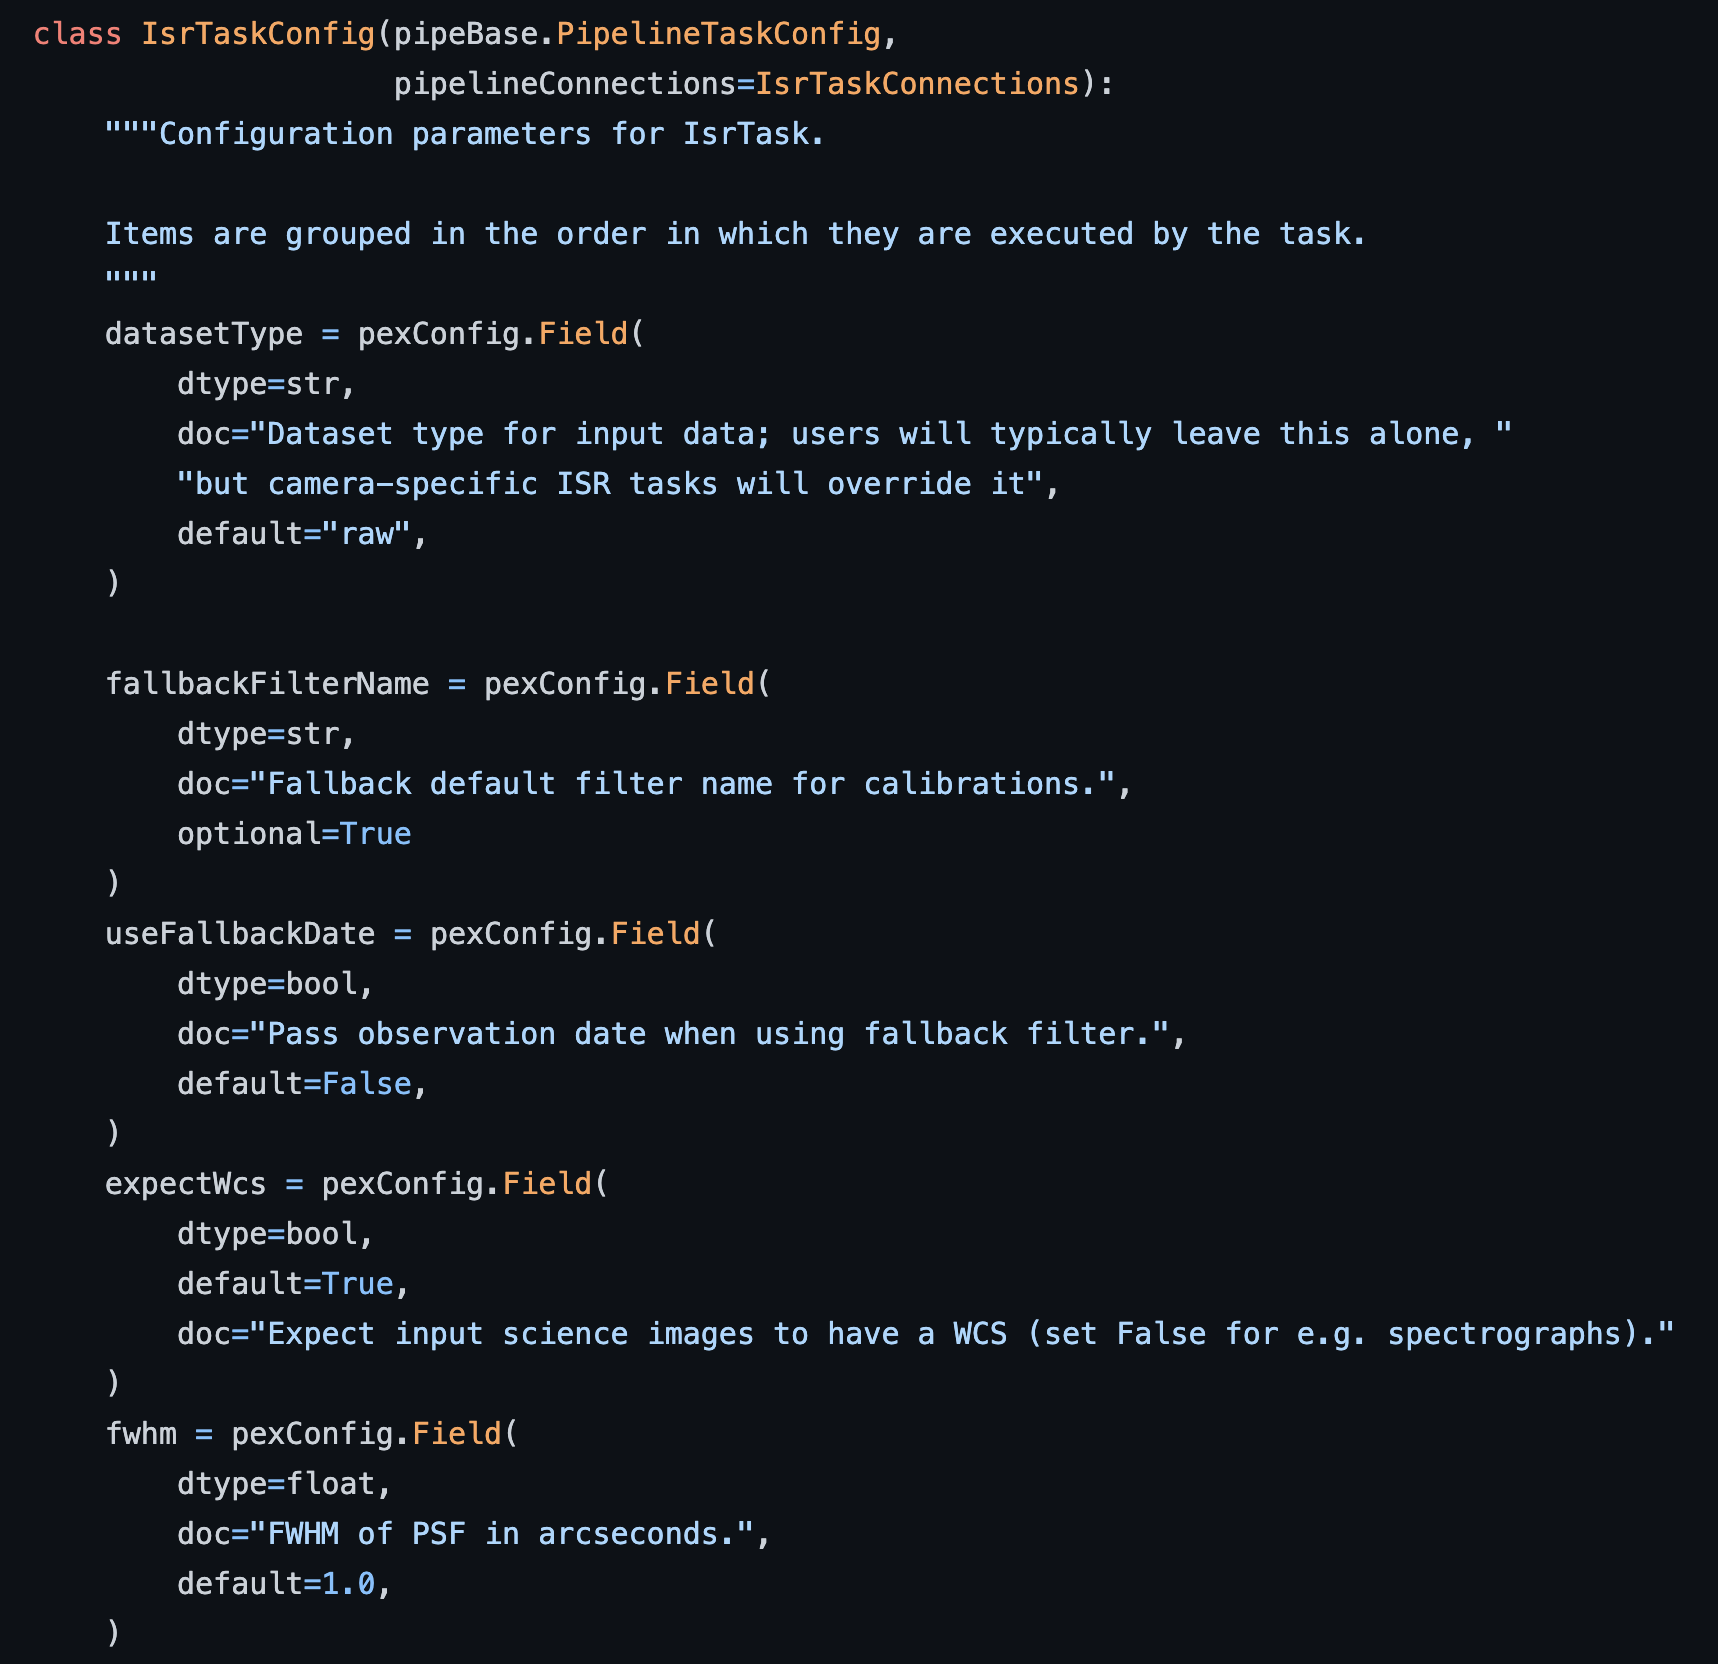
\includegraphics[width=3.12500in]{jira_imgs/3072.png}\\
These configuration parameters can be changed in a .yaml pipeline that
is invoked at pipetask runtime.~

}
\begin{tabular}{p{2cm}p{14cm}}
\toprule
Step 2 & Step Execution Status: \textbf{ Pass } \\ \hline
\end{tabular}
 Description \\
{\footnotesize
Verify that tasks can consist of multiple subtasks chained together.

}
\hdashrule[0.5ex]{\textwidth}{1pt}{3mm}
  Expected Result \\
{\footnotesize
Confirmation that the software architecture has allowed for the use of
subsets and chains of tasks.

}
\hdashrule[0.5ex]{\textwidth}{1pt}{3mm}
  Actual Result \\
{\footnotesize
An example of a YAML pipeline (in this case, one that calculates the
crosstalk correction) is seen below. One can see that it satisfies the
requirement from step 1 that the configuration parameters can be
specified without recompilation of code. At the bottom, this excerpt
also shows an example of subtasks being chained together to create
larger
tasks.\\[2\baselineskip]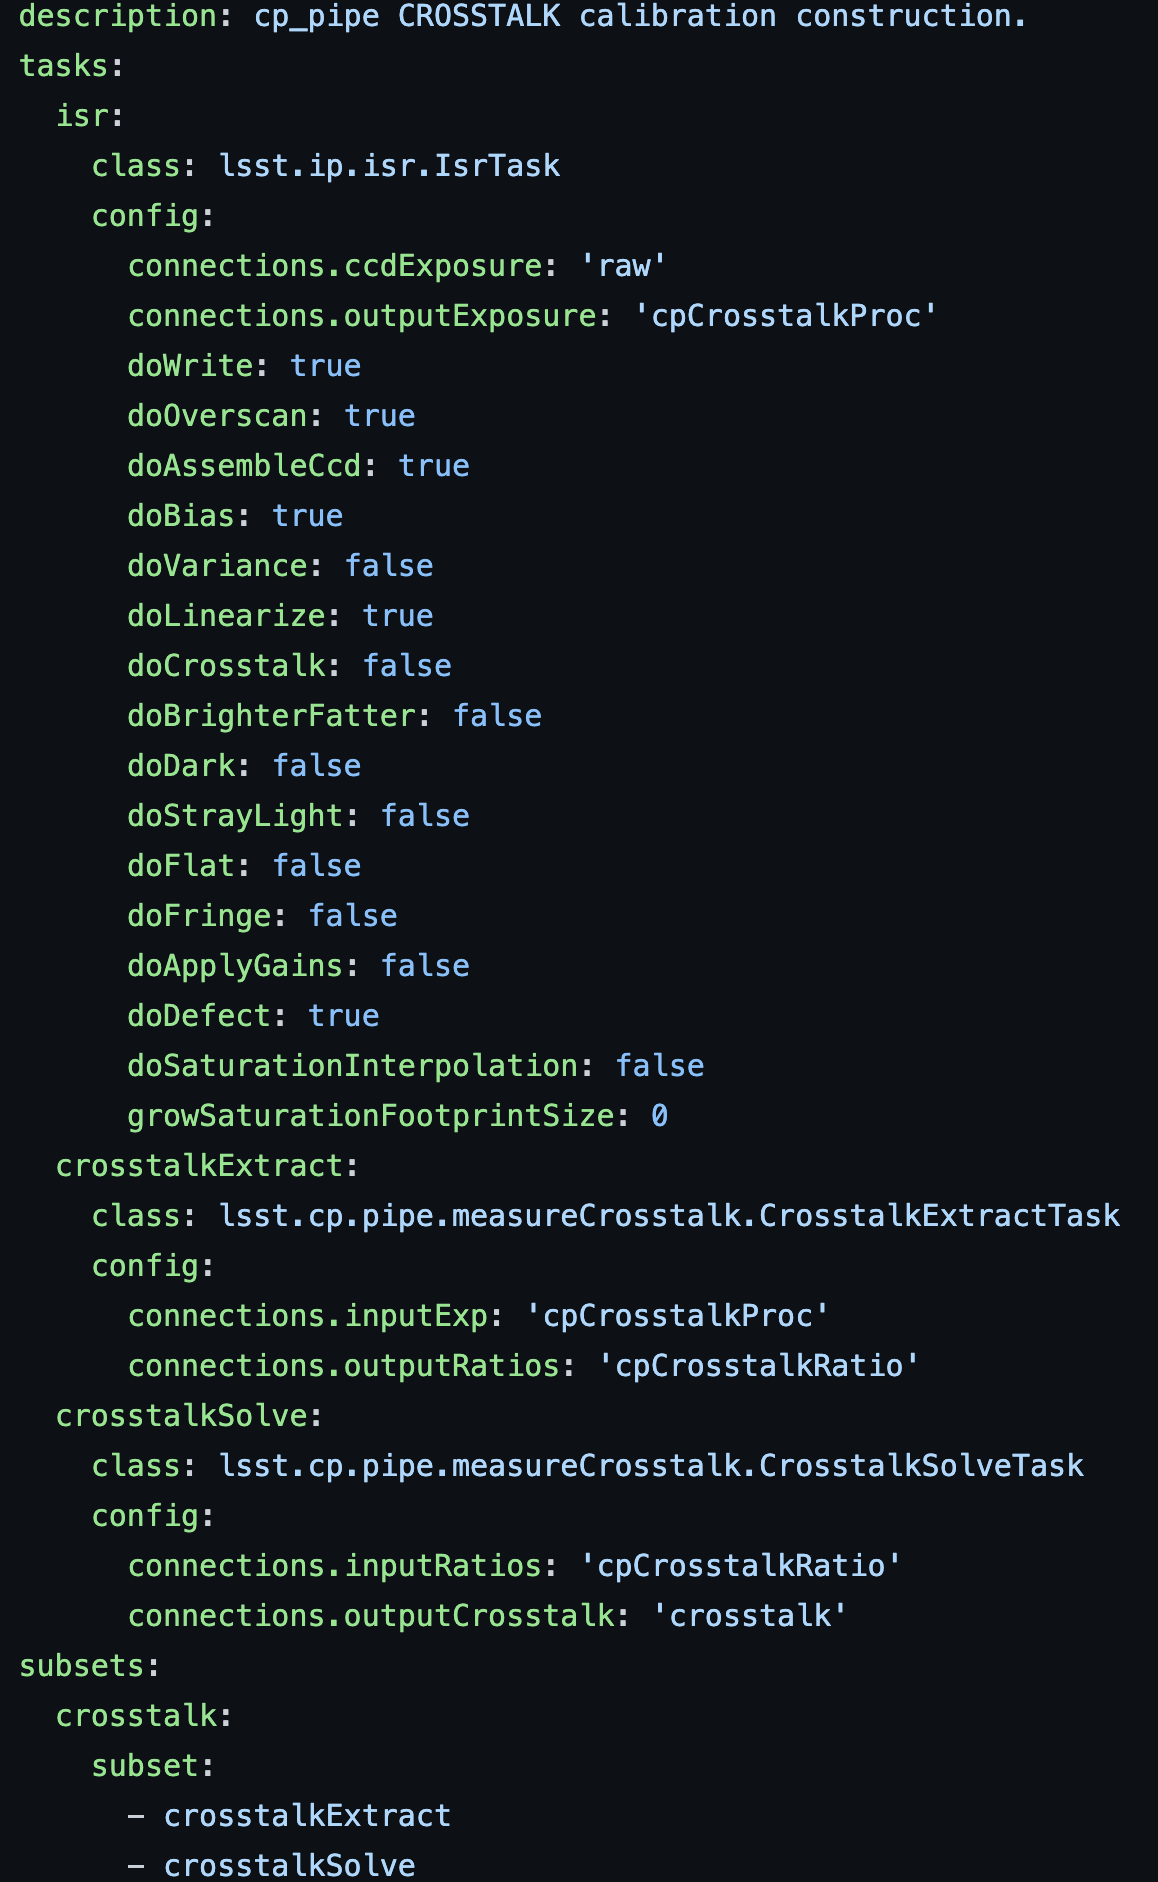
\includegraphics[width=4.20833in]{jira_imgs/3074.png}

}
\begin{tabular}{p{2cm}p{14cm}}
\toprule
Step 3 & Step Execution Status: \textbf{ Pass } \\ \hline
\end{tabular}
 Description \\
{\footnotesize
Verify that an example science algorithm can be run through one of these
Tasks.

}
\hdashrule[0.5ex]{\textwidth}{1pt}{3mm}
  Expected Result \\
{\footnotesize
Successful Task execution with different configurations, including
confirmation that the outputs are different from tasks with altered
configurations.

}
\hdashrule[0.5ex]{\textwidth}{1pt}{3mm}
  Actual Result \\
{\footnotesize
For this, we refer to verification performed in
\href{https://jira.lsstcorp.org/secure/Tests.jspa\#/testCase/257}{LVV-T145},
where we demonstrated that configurations can be changed in YAML
specification files, and that these changes can be demonstrated to take
effect.\\[2\baselineskip]Executing the script from LVV-T145 prints the
following to the screen:\\
python test\_LVV-T145.py\\[2\baselineskip]lsst\_distrib
g0b29ad24fb+434521fcbd current w\_2022\_35 setup\\
src1 length: 3172\\
src2 length: 3212\\
run1 threshold: 100.0\\
run2 threshold: 30.0\\[2\baselineskip]\ldots{}where run1 and run2 were
source detection runs using detection thresholds of 100 and
30.\\[2\baselineskip]This confirms that the change in threshold affected
the number of detected sources, and that the thresholds were persisted
in metadata in the butler collections.

}

\paragraph{ LVV-T74 - Verify implementation of Template Coadds }\mbox{}\\

Version \textbf{1}.
Status \textbf{Approved}.
Open  \href{https://jira.lsstcorp.org/secure/Tests.jspa#/testCase/LVV-T74}{\textit{ LVV-T74 } }
test case in Jira.

Verify that the DMS can produce Template Coadds for DIA processing.

\textbf{ Preconditions}:\\


Execution status: {\bf Pass }

Final comment:\\See attached artifact notebook ``test\_LVV-T74.ipynb'' for details.


Detailed steps results:

\begin{tabular}{p{2cm}p{14cm}}
\toprule
Step 1 & Step Execution Status: \textbf{ Pass } \\ \hline
\end{tabular}
 Description \\
{\footnotesize
Perform the steps of Alert Production (including, but not necessarily
limited to, single frame processing, ISR, source detection/measurement,
PSF estimation, photometric and astrometric calibration, difference
imaging, DIASource detection/measurement, source association). During
Operations, it is presumed that these are automated for a given
dataset.~

}
\hdashrule[0.5ex]{\textwidth}{1pt}{3mm}
  Expected Result \\
{\footnotesize
An output dataset including difference images and DIASource and
DIAObject measurements.

}
\hdashrule[0.5ex]{\textwidth}{1pt}{3mm}
  Actual Result \\
{\footnotesize
Logged into the RSP at the Interim Data Facility, and accessed the
shared butler repositories containing Data Preview 0.2 data. All work
for this Test Case is in Jupyter notebook ``test\_LVV-T74.ipynb'', which
is archived along with the test report.

}
\begin{tabular}{p{2cm}p{14cm}}
\toprule
Step 2 & Step Execution Status: \textbf{ Pass } \\ \hline
\end{tabular}
 Description \\
{\footnotesize
Verify that the expected data products have been produced, and that
catalogs contain reasonable values for measured quantities of interest.

}
\hdashrule[0.5ex]{\textwidth}{1pt}{3mm}
  Expected Result \\
{\footnotesize

}
\hdashrule[0.5ex]{\textwidth}{1pt}{3mm}
  Actual Result \\
{\footnotesize
We confirmed that the expected data products are present, including
DIASource tables, DIAObject measurements and their associations with
DIASource, template images, and that all have been photometrically and
astrometrically calibrated.

}
\begin{tabular}{p{2cm}p{14cm}}
\toprule
Step 3 & Step Execution Status: \textbf{ Pass } \\ \hline
\end{tabular}
 Description \\
{\footnotesize
Confirm that the template coadds have been created and are well-formed.

}
\hdashrule[0.5ex]{\textwidth}{1pt}{3mm}
  Expected Result \\
{\footnotesize

}
\hdashrule[0.5ex]{\textwidth}{1pt}{3mm}
  Actual Result \\
{\footnotesize
Finally, we displayed a template coadd and compared it to the original
image. See notebook ``test\_LVV-T74.ipynb'' for details.

}




% This appendix is put in as part of the template. You may edit and add to it.
% It is not overwritten by Docsteady.

\newpage
\appendix
\section{Documentation}
The verification process is defined in \citeds{LSE-160}.
The use of Docsteady to format Jira information in various test and planing documents is
described in \citeds{DMTN-140} and practical commands are given in \citeds{DMTN-178}.

\section{Acronyms used in this document}\label{sec:acronyms}
\input{acronyms.tex}

\newpage

% Uncomment this if Docsteady makes you additional appendix
%\input{DMTR-371.appendix.tex}

\end{document}
